\documentclass[twoside]{book}

% Packages required by doxygen
\usepackage{fixltx2e}
\usepackage{calc}
\usepackage{doxygen}
\usepackage[export]{adjustbox} % also loads graphicx
\usepackage{graphicx}
\usepackage[utf8]{inputenc}
\usepackage{makeidx}
\usepackage{multicol}
\usepackage{multirow}
\PassOptionsToPackage{warn}{textcomp}
\usepackage{textcomp}
\usepackage[nointegrals]{wasysym}
\usepackage[table]{xcolor}

% Font selection
\usepackage[T1]{fontenc}
\usepackage[scaled=.90]{helvet}
\usepackage{courier}
\usepackage{amssymb}
\usepackage{sectsty}
\renewcommand{\familydefault}{\sfdefault}
\allsectionsfont{%
  \fontseries{bc}\selectfont%
  \color{darkgray}%
}
\renewcommand{\DoxyLabelFont}{%
  \fontseries{bc}\selectfont%
  \color{darkgray}%
}
\newcommand{\+}{\discretionary{\mbox{\scriptsize$\hookleftarrow$}}{}{}}

% Page & text layout
\usepackage{geometry}
\geometry{%
  a4paper,%
  top=2.5cm,%
  bottom=2.5cm,%
  left=2.5cm,%
  right=2.5cm%
}
\tolerance=750
\hfuzz=15pt
\hbadness=750
\setlength{\emergencystretch}{15pt}
\setlength{\parindent}{0cm}
\setlength{\parskip}{3ex plus 2ex minus 2ex}
\makeatletter
\renewcommand{\paragraph}{%
  \@startsection{paragraph}{4}{0ex}{-1.0ex}{1.0ex}{%
    \normalfont\normalsize\bfseries\SS@parafont%
  }%
}
\renewcommand{\subparagraph}{%
  \@startsection{subparagraph}{5}{0ex}{-1.0ex}{1.0ex}{%
    \normalfont\normalsize\bfseries\SS@subparafont%
  }%
}
\makeatother

% Headers & footers
\usepackage{fancyhdr}
\pagestyle{fancyplain}
\fancyhead[LE]{\fancyplain{}{\bfseries\thepage}}
\fancyhead[CE]{\fancyplain{}{}}
\fancyhead[RE]{\fancyplain{}{\bfseries\leftmark}}
\fancyhead[LO]{\fancyplain{}{\bfseries\rightmark}}
\fancyhead[CO]{\fancyplain{}{}}
\fancyhead[RO]{\fancyplain{}{\bfseries\thepage}}
\fancyfoot[LE]{\fancyplain{}{}}
\fancyfoot[CE]{\fancyplain{}{}}
\fancyfoot[RE]{\fancyplain{}{\bfseries\scriptsize Generated by Doxygen }}
\fancyfoot[LO]{\fancyplain{}{\bfseries\scriptsize Generated by Doxygen }}
\fancyfoot[CO]{\fancyplain{}{}}
\fancyfoot[RO]{\fancyplain{}{}}
\renewcommand{\footrulewidth}{0.4pt}
\renewcommand{\chaptermark}[1]{%
  \markboth{#1}{}%
}
\renewcommand{\sectionmark}[1]{%
  \markright{\thesection\ #1}%
}

% Indices & bibliography
\usepackage{natbib}
\usepackage[titles]{tocloft}
\setcounter{tocdepth}{3}
\setcounter{secnumdepth}{5}
\makeindex

% Hyperlinks (required, but should be loaded last)
\usepackage{ifpdf}
\ifpdf
  \usepackage[pdftex,pagebackref=true]{hyperref}
\else
  \usepackage[ps2pdf,pagebackref=true]{hyperref}
\fi
\hypersetup{%
  colorlinks=true,%
  linkcolor=blue,%
  citecolor=blue,%
  unicode%
}

% Custom commands
\newcommand{\clearemptydoublepage}{%
  \newpage{\pagestyle{empty}\cleardoublepage}%
}

\usepackage{caption}
\captionsetup{labelsep=space,justification=centering,font={bf},singlelinecheck=off,skip=4pt,position=top}

%===== C O N T E N T S =====

\begin{document}

% Titlepage & ToC
\hypersetup{pageanchor=false,
             bookmarksnumbered=true,
             pdfencoding=unicode
            }
\pagenumbering{alph}
\begin{titlepage}
\vspace*{7cm}
\begin{center}%
{\Large My Project \\[1ex]\large 1.\+0 }\\
\vspace*{1cm}
{\large Generated by Doxygen 1.8.13}\\
\end{center}
\end{titlepage}
\clearemptydoublepage
\pagenumbering{roman}
\tableofcontents
\clearemptydoublepage
\pagenumbering{arabic}
\hypersetup{pageanchor=true}

%--- Begin generated contents ---
\chapter{Hierarchical Index}
\section{Class Hierarchy}
This inheritance list is sorted roughly, but not completely, alphabetically\+:\begin{DoxyCompactList}
\item \contentsline{section}{Already\+Paid}{\pageref{classAlreadyPaid}}{}
\item \contentsline{section}{Area}{\pageref{classArea}}{}
\item \contentsline{section}{Associate}{\pageref{classAssociate}}{}
\item \contentsline{section}{Association}{\pageref{classAssociation}}{}
\item \contentsline{section}{Event}{\pageref{classEvent}}{}
\begin{DoxyCompactList}
\item \contentsline{section}{Conference}{\pageref{classConference}}{}
\item \contentsline{section}{Summer\+School}{\pageref{classSummerSchool}}{}
\end{DoxyCompactList}
\item \contentsline{section}{inactive\+Associate\+Hash}{\pageref{structinactiveAssociateHash}}{}
\item \contentsline{section}{Invalid\+Request}{\pageref{classInvalidRequest}}{}
\item \contentsline{section}{Mail}{\pageref{classMail}}{}
\item \contentsline{section}{Network}{\pageref{classNetwork}}{}
\item \contentsline{section}{No\+Such\+Date}{\pageref{classNoSuchDate}}{}
\item \contentsline{section}{No\+Such\+ID}{\pageref{classNoSuchID}}{}
\item \contentsline{section}{Not\+Enough\+Money}{\pageref{classNotEnoughMoney}}{}
\item \contentsline{section}{Not\+Up\+To\+Date}{\pageref{classNotUpToDate}}{}
\item \contentsline{section}{Sub\+Area}{\pageref{classSubArea}}{}
\item \contentsline{section}{Trainer}{\pageref{classTrainer}}{}
\end{DoxyCompactList}

\chapter{Class Index}
\section{Class List}
Here are the classes, structs, unions and interfaces with brief descriptions\+:\begin{DoxyCompactList}
\item\contentsline{section}{\hyperlink{classAlreadyPaid}{Already\+Paid} \\*The Not\+Already\+Paid Class }{\pageref{classAlreadyPaid}}{}
\item\contentsline{section}{\hyperlink{classArea}{Area} \\*The \hyperlink{classArea}{Area} Class }{\pageref{classArea}}{}
\item\contentsline{section}{\hyperlink{classAssociate}{Associate} \\*The \hyperlink{classAssociate}{Associate} Class }{\pageref{classAssociate}}{}
\item\contentsline{section}{\hyperlink{classAssociation}{Association} \\*The \hyperlink{classAssociation}{Association} Class }{\pageref{classAssociation}}{}
\item\contentsline{section}{\hyperlink{classConference}{Conference} \\*The \hyperlink{classConference}{Conference} Class -\/ Derived Class from the Super \hyperlink{classEvent}{Event} Class }{\pageref{classConference}}{}
\item\contentsline{section}{\hyperlink{classEvent}{Event} \\*The Super \hyperlink{classEvent}{Event} Class }{\pageref{classEvent}}{}
\item\contentsline{section}{\hyperlink{classMail}{Mail} \\*The \hyperlink{classMail}{Mail} Class }{\pageref{classMail}}{}
\item\contentsline{section}{\hyperlink{classNetwork}{Network} \\*The \hyperlink{classNetwork}{Network} Class }{\pageref{classNetwork}}{}
\item\contentsline{section}{\hyperlink{classNoSuchDate}{No\+Such\+Date} \\*The \hyperlink{classNoSuchDate}{No\+Such\+Date} Class }{\pageref{classNoSuchDate}}{}
\item\contentsline{section}{\hyperlink{classNoSuchID}{No\+Such\+ID} \\*The \hyperlink{classNoSuchID}{No\+Such\+ID} Class }{\pageref{classNoSuchID}}{}
\item\contentsline{section}{\hyperlink{classNoSupportGiven}{No\+Support\+Given} \\*The \hyperlink{classNoSupportGiven}{No\+Support\+Given} }{\pageref{classNoSupportGiven}}{}
\item\contentsline{section}{\hyperlink{classNotEnoughMoney}{Not\+Enough\+Money} \\*The \hyperlink{classNotEnoughMoney}{Not\+Enough\+Money} Class }{\pageref{classNotEnoughMoney}}{}
\item\contentsline{section}{\hyperlink{classNotUpToDate}{Not\+Up\+To\+Date} \\*The \hyperlink{classNotUpToDate}{Not\+Up\+To\+Date} Class }{\pageref{classNotUpToDate}}{}
\item\contentsline{section}{\hyperlink{classSubArea}{Sub\+Area} \\*The \hyperlink{classSubArea}{Sub\+Area} Class }{\pageref{classSubArea}}{}
\item\contentsline{section}{\hyperlink{classSummerSchool}{Summer\+School} \\*The \hyperlink{classSummerSchool}{Summer\+School} Class -\/ Derived Class from the Super \hyperlink{classEvent}{Event} Class }{\pageref{classSummerSchool}}{}
\item\contentsline{section}{\hyperlink{classTrainer}{Trainer} \\*The \hyperlink{classTrainer}{Trainer} Class }{\pageref{classTrainer}}{}
\end{DoxyCompactList}

\chapter{File Index}
\section{File List}
Here is a list of all files with brief descriptions\+:\begin{DoxyCompactList}
\item\contentsline{section}{\hyperlink{Area_8cpp}{Area.\+cpp} }{\pageref{Area_8cpp}}{}
\item\contentsline{section}{\hyperlink{Area_8h}{Area.\+h} }{\pageref{Area_8h}}{}
\item\contentsline{section}{\hyperlink{Associate_8cpp}{Associate.\+cpp} }{\pageref{Associate_8cpp}}{}
\item\contentsline{section}{\hyperlink{Associate_8h}{Associate.\+h} }{\pageref{Associate_8h}}{}
\item\contentsline{section}{\hyperlink{Association_8cpp}{Association.\+cpp} }{\pageref{Association_8cpp}}{}
\item\contentsline{section}{\hyperlink{Association_8h}{Association.\+h} }{\pageref{Association_8h}}{}
\item\contentsline{section}{\hyperlink{Conference_8cpp}{Conference.\+cpp} }{\pageref{Conference_8cpp}}{}
\item\contentsline{section}{\hyperlink{Conference_8h}{Conference.\+h} }{\pageref{Conference_8h}}{}
\item\contentsline{section}{\hyperlink{Event_8cpp}{Event.\+cpp} }{\pageref{Event_8cpp}}{}
\item\contentsline{section}{\hyperlink{Event_8h}{Event.\+h} }{\pageref{Event_8h}}{}
\item\contentsline{section}{\hyperlink{Functions_8cpp}{Functions.\+cpp} }{\pageref{Functions_8cpp}}{}
\item\contentsline{section}{\hyperlink{Functions_8h}{Functions.\+h} }{\pageref{Functions_8h}}{}
\item\contentsline{section}{\hyperlink{Mail_8cpp}{Mail.\+cpp} }{\pageref{Mail_8cpp}}{}
\item\contentsline{section}{\hyperlink{Mail_8h}{Mail.\+h} }{\pageref{Mail_8h}}{}
\item\contentsline{section}{\hyperlink{main_8cpp}{main.\+cpp} }{\pageref{main_8cpp}}{}
\item\contentsline{section}{\hyperlink{menu_8cpp}{menu.\+cpp} }{\pageref{menu_8cpp}}{}
\item\contentsline{section}{\hyperlink{menu_8h}{menu.\+h} }{\pageref{menu_8h}}{}
\item\contentsline{section}{\hyperlink{Network_8cpp}{Network.\+cpp} }{\pageref{Network_8cpp}}{}
\item\contentsline{section}{\hyperlink{Network_8h}{Network.\+h} }{\pageref{Network_8h}}{}
\item\contentsline{section}{\hyperlink{SubArea_8cpp}{Sub\+Area.\+cpp} }{\pageref{SubArea_8cpp}}{}
\item\contentsline{section}{\hyperlink{SubArea_8h}{Sub\+Area.\+h} }{\pageref{SubArea_8h}}{}
\item\contentsline{section}{\hyperlink{SummerSchool_8cpp}{Summer\+School.\+cpp} }{\pageref{SummerSchool_8cpp}}{}
\item\contentsline{section}{\hyperlink{SummerSchool_8h}{Summer\+School.\+h} }{\pageref{SummerSchool_8h}}{}
\end{DoxyCompactList}

\chapter{Class Documentation}
\hypertarget{classAlreadyPaid}{}\section{Already\+Paid Class Reference}
\label{classAlreadyPaid}\index{Already\+Paid@{Already\+Paid}}


The Not\+Already\+Paid Class.  




{\ttfamily \#include $<$Associate.\+h$>$}

\subsection*{Public Member Functions}
\begin{DoxyCompactItemize}
\item 
\hyperlink{classAlreadyPaid_afa3ccdeb73e3570b346a4938a836a44e}{Already\+Paid} (int \hyperlink{classAlreadyPaid_aca0124c0c69671e1452020fc8697c3ca}{year}, int \hyperlink{classAlreadyPaid_ad5c108176759cfd9d2f9ca2dd143d843}{unique\+ID})
\begin{DoxyCompactList}\small\item\em Full \hyperlink{classAlreadyPaid}{Already\+Paid} Constructor. \end{DoxyCompactList}\item 
int \hyperlink{classAlreadyPaid_a54d1869f925f98bb8621131debf5f2c8}{get\+ID} () const
\begin{DoxyCompactList}\small\item\em Returns the id of the associate trying to pay the annual pay. \end{DoxyCompactList}\item 
int \hyperlink{classAlreadyPaid_a9bc932f3c57052ce0508abc48b5a5a6c}{get\+Year} () const
\begin{DoxyCompactList}\small\item\em Returns the year the associate is trying to pay. \end{DoxyCompactList}\end{DoxyCompactItemize}
\subsection*{Private Attributes}
\begin{DoxyCompactItemize}
\item 
int \hyperlink{classAlreadyPaid_aca0124c0c69671e1452020fc8697c3ca}{year}
\begin{DoxyCompactList}\small\item\em The year the associate is trying to pay. \end{DoxyCompactList}\item 
int \hyperlink{classAlreadyPaid_ad5c108176759cfd9d2f9ca2dd143d843}{unique\+ID}
\begin{DoxyCompactList}\small\item\em The id of the associate who is trying to pay the annual pay. \end{DoxyCompactList}\end{DoxyCompactItemize}


\subsection{Detailed Description}
The Not\+Already\+Paid Class. 

\hyperlink{classAlreadyPaid}{Already\+Paid} is a class which instances are called when an associate tries to pay the annual pay of an year he has already paid. Its useful in throwing exceptions, outside of that it has no real use. 

\subsection{Constructor \& Destructor Documentation}
\mbox{\Hypertarget{classAlreadyPaid_afa3ccdeb73e3570b346a4938a836a44e}\label{classAlreadyPaid_afa3ccdeb73e3570b346a4938a836a44e}} 
\index{Already\+Paid@{Already\+Paid}!Already\+Paid@{Already\+Paid}}
\index{Already\+Paid@{Already\+Paid}!Already\+Paid@{Already\+Paid}}
\subsubsection{\texorpdfstring{Already\+Paid()}{AlreadyPaid()}}
{\footnotesize\ttfamily Already\+Paid\+::\+Already\+Paid (\begin{DoxyParamCaption}\item[{int}]{year,  }\item[{int}]{unique\+ID }\end{DoxyParamCaption})\hspace{0.3cm}{\ttfamily [inline]}}



Full \hyperlink{classAlreadyPaid}{Already\+Paid} Constructor. 


\begin{DoxyParams}{Parameters}
{\em year} & -\/ The year the associate is trying to pay \\
\hline
{\em unique\+ID} & -\/ The id of the associate who is trying to pay the annual pay \\
\hline
\end{DoxyParams}


\subsection{Member Function Documentation}
\mbox{\Hypertarget{classAlreadyPaid_a54d1869f925f98bb8621131debf5f2c8}\label{classAlreadyPaid_a54d1869f925f98bb8621131debf5f2c8}} 
\index{Already\+Paid@{Already\+Paid}!get\+ID@{get\+ID}}
\index{get\+ID@{get\+ID}!Already\+Paid@{Already\+Paid}}
\subsubsection{\texorpdfstring{get\+I\+D()}{getID()}}
{\footnotesize\ttfamily int Already\+Paid\+::get\+ID (\begin{DoxyParamCaption}{ }\end{DoxyParamCaption}) const\hspace{0.3cm}{\ttfamily [inline]}}



Returns the id of the associate trying to pay the annual pay. 

\mbox{\Hypertarget{classAlreadyPaid_a9bc932f3c57052ce0508abc48b5a5a6c}\label{classAlreadyPaid_a9bc932f3c57052ce0508abc48b5a5a6c}} 
\index{Already\+Paid@{Already\+Paid}!get\+Year@{get\+Year}}
\index{get\+Year@{get\+Year}!Already\+Paid@{Already\+Paid}}
\subsubsection{\texorpdfstring{get\+Year()}{getYear()}}
{\footnotesize\ttfamily int Already\+Paid\+::get\+Year (\begin{DoxyParamCaption}{ }\end{DoxyParamCaption}) const\hspace{0.3cm}{\ttfamily [inline]}}



Returns the year the associate is trying to pay. 



\subsection{Member Data Documentation}
\mbox{\Hypertarget{classAlreadyPaid_ad5c108176759cfd9d2f9ca2dd143d843}\label{classAlreadyPaid_ad5c108176759cfd9d2f9ca2dd143d843}} 
\index{Already\+Paid@{Already\+Paid}!unique\+ID@{unique\+ID}}
\index{unique\+ID@{unique\+ID}!Already\+Paid@{Already\+Paid}}
\subsubsection{\texorpdfstring{unique\+ID}{uniqueID}}
{\footnotesize\ttfamily int Already\+Paid\+::unique\+ID\hspace{0.3cm}{\ttfamily [private]}}



The id of the associate who is trying to pay the annual pay. 

\mbox{\Hypertarget{classAlreadyPaid_aca0124c0c69671e1452020fc8697c3ca}\label{classAlreadyPaid_aca0124c0c69671e1452020fc8697c3ca}} 
\index{Already\+Paid@{Already\+Paid}!year@{year}}
\index{year@{year}!Already\+Paid@{Already\+Paid}}
\subsubsection{\texorpdfstring{year}{year}}
{\footnotesize\ttfamily int Already\+Paid\+::year\hspace{0.3cm}{\ttfamily [private]}}



The year the associate is trying to pay. 



The documentation for this class was generated from the following file\+:\begin{DoxyCompactItemize}
\item 
\hyperlink{Associate_8h}{Associate.\+h}\end{DoxyCompactItemize}

\hypertarget{classArea}{}\section{Area Class Reference}
\label{classArea}\index{Area@{Area}}


The \mbox{\hyperlink{classArea}{Area}} Class.  




{\ttfamily \#include $<$Area.\+h$>$}

\subsection*{Public Member Functions}
\begin{DoxyCompactItemize}
\item 
\mbox{\hyperlink{classArea_aa92851fcffb0a9f1c6c8c283204f7003}{Area}} ()
\begin{DoxyCompactList}\small\item\em Default Constructor. \end{DoxyCompactList}\item 
\mbox{\hyperlink{classArea_afd32499f2246ef8007fd135d7503da16}{Area}} (std\+::string file\+\_\+string)
\begin{DoxyCompactList}\small\item\em File Constructor. \end{DoxyCompactList}\item 
virtual \mbox{\hyperlink{classArea_ace0975982b61a16746c564a0d43a4cc8}{$\sim$\+Area}} ()
\begin{DoxyCompactList}\small\item\em Default Destructor. \end{DoxyCompactList}\item 
std\+::string \mbox{\hyperlink{classArea_acdbc3527be262d1ea1b9c961e823257f}{get\+Name}} () const
\begin{DoxyCompactList}\small\item\em Returns the name of the \mbox{\hyperlink{classArea}{Area}}. \end{DoxyCompactList}\item 
std\+::vector$<$ \mbox{\hyperlink{classSubArea}{Sub\+Area}} $\ast$ $>$ \mbox{\hyperlink{classArea_abf3bfb978d0a7d05fe2cbbad9ce7fef4}{get\+Sub\+Areas}} () const
\begin{DoxyCompactList}\small\item\em Returns the subareas of the \mbox{\hyperlink{classArea}{Area}}. \end{DoxyCompactList}\item 
void \mbox{\hyperlink{classArea_a137ad0664d3993ff994e2381804459e2}{add\+Subarea}} (\mbox{\hyperlink{classSubArea}{Sub\+Area}} $\ast$new\+Sub)
\begin{DoxyCompactList}\small\item\em Adds a \mbox{\hyperlink{classSubArea}{Sub\+Area}} to the vector containing all the Sub\+Areas of the \mbox{\hyperlink{classArea}{Area}}. \end{DoxyCompactList}\end{DoxyCompactItemize}
\subsection*{Private Attributes}
\begin{DoxyCompactItemize}
\item 
std\+::string \mbox{\hyperlink{classArea_a24201719de9d9dfef7a720c036529dd7}{name}}
\begin{DoxyCompactList}\small\item\em The \mbox{\hyperlink{classArea}{Area}}\textquotesingle{}s name. \end{DoxyCompactList}\item 
std\+::vector$<$ \mbox{\hyperlink{classSubArea}{Sub\+Area}} $\ast$ $>$ \mbox{\hyperlink{classArea_af5eafd40b41ae847a009feef631ce07f}{subareas}}
\begin{DoxyCompactList}\small\item\em The \mbox{\hyperlink{classArea}{Area}}\textquotesingle{}s Sub\+Areas. \end{DoxyCompactList}\end{DoxyCompactItemize}


\subsection{Detailed Description}
The \mbox{\hyperlink{classArea}{Area}} Class. 

An \mbox{\hyperlink{classAssociation}{Association}} consists in a group of associates. Each associate has interest in a variety of areas. Each area has some subareas. An area is distinguished by its name 

\subsection{Constructor \& Destructor Documentation}
\mbox{\Hypertarget{classArea_aa92851fcffb0a9f1c6c8c283204f7003}\label{classArea_aa92851fcffb0a9f1c6c8c283204f7003}} 
\index{Area@{Area}!Area@{Area}}
\index{Area@{Area}!Area@{Area}}
\subsubsection{\texorpdfstring{Area()}{Area()}\hspace{0.1cm}{\footnotesize\ttfamily [1/2]}}
{\footnotesize\ttfamily Area\+::\+Area (\begin{DoxyParamCaption}{ }\end{DoxyParamCaption})}



Default Constructor. 

\mbox{\Hypertarget{classArea_afd32499f2246ef8007fd135d7503da16}\label{classArea_afd32499f2246ef8007fd135d7503da16}} 
\index{Area@{Area}!Area@{Area}}
\index{Area@{Area}!Area@{Area}}
\subsubsection{\texorpdfstring{Area()}{Area()}\hspace{0.1cm}{\footnotesize\ttfamily [2/2]}}
{\footnotesize\ttfamily Area\+::\+Area (\begin{DoxyParamCaption}\item[{std\+::string}]{file\+\_\+string }\end{DoxyParamCaption})}



File Constructor. 


\begin{DoxyParams}{Parameters}
{\em file\+\_\+string} & -\/ Reads a line from a file and creates the area and its subareas based on that information \\
\hline
\end{DoxyParams}
\mbox{\Hypertarget{classArea_ace0975982b61a16746c564a0d43a4cc8}\label{classArea_ace0975982b61a16746c564a0d43a4cc8}} 
\index{Area@{Area}!````~Area@{$\sim$\+Area}}
\index{````~Area@{$\sim$\+Area}!Area@{Area}}
\subsubsection{\texorpdfstring{$\sim$\+Area()}{~Area()}}
{\footnotesize\ttfamily Area\+::$\sim$\+Area (\begin{DoxyParamCaption}{ }\end{DoxyParamCaption})\hspace{0.3cm}{\ttfamily [virtual]}}



Default Destructor. 



\subsection{Member Function Documentation}
\mbox{\Hypertarget{classArea_a137ad0664d3993ff994e2381804459e2}\label{classArea_a137ad0664d3993ff994e2381804459e2}} 
\index{Area@{Area}!add\+Subarea@{add\+Subarea}}
\index{add\+Subarea@{add\+Subarea}!Area@{Area}}
\subsubsection{\texorpdfstring{add\+Subarea()}{addSubarea()}}
{\footnotesize\ttfamily void Area\+::add\+Subarea (\begin{DoxyParamCaption}\item[{\mbox{\hyperlink{classSubArea}{Sub\+Area}} $\ast$}]{new\+Sub }\end{DoxyParamCaption})}



Adds a \mbox{\hyperlink{classSubArea}{Sub\+Area}} to the vector containing all the Sub\+Areas of the \mbox{\hyperlink{classArea}{Area}}. 


\begin{DoxyParams}{Parameters}
{\em new\+Sub} & -\/ The \mbox{\hyperlink{classSubArea}{Sub\+Area}} that is supposed to add to the vector \\
\hline
\end{DoxyParams}
\mbox{\Hypertarget{classArea_acdbc3527be262d1ea1b9c961e823257f}\label{classArea_acdbc3527be262d1ea1b9c961e823257f}} 
\index{Area@{Area}!get\+Name@{get\+Name}}
\index{get\+Name@{get\+Name}!Area@{Area}}
\subsubsection{\texorpdfstring{get\+Name()}{getName()}}
{\footnotesize\ttfamily string Area\+::get\+Name (\begin{DoxyParamCaption}{ }\end{DoxyParamCaption}) const}



Returns the name of the \mbox{\hyperlink{classArea}{Area}}. 

\mbox{\Hypertarget{classArea_abf3bfb978d0a7d05fe2cbbad9ce7fef4}\label{classArea_abf3bfb978d0a7d05fe2cbbad9ce7fef4}} 
\index{Area@{Area}!get\+Sub\+Areas@{get\+Sub\+Areas}}
\index{get\+Sub\+Areas@{get\+Sub\+Areas}!Area@{Area}}
\subsubsection{\texorpdfstring{get\+Sub\+Areas()}{getSubAreas()}}
{\footnotesize\ttfamily vector$<$ \mbox{\hyperlink{classSubArea}{Sub\+Area}} $\ast$ $>$ Area\+::get\+Sub\+Areas (\begin{DoxyParamCaption}{ }\end{DoxyParamCaption}) const}



Returns the subareas of the \mbox{\hyperlink{classArea}{Area}}. 



\subsection{Member Data Documentation}
\mbox{\Hypertarget{classArea_a24201719de9d9dfef7a720c036529dd7}\label{classArea_a24201719de9d9dfef7a720c036529dd7}} 
\index{Area@{Area}!name@{name}}
\index{name@{name}!Area@{Area}}
\subsubsection{\texorpdfstring{name}{name}}
{\footnotesize\ttfamily std\+::string Area\+::name\hspace{0.3cm}{\ttfamily [private]}}



The \mbox{\hyperlink{classArea}{Area}}\textquotesingle{}s name. 

\mbox{\Hypertarget{classArea_af5eafd40b41ae847a009feef631ce07f}\label{classArea_af5eafd40b41ae847a009feef631ce07f}} 
\index{Area@{Area}!subareas@{subareas}}
\index{subareas@{subareas}!Area@{Area}}
\subsubsection{\texorpdfstring{subareas}{subareas}}
{\footnotesize\ttfamily std\+::vector$<$\mbox{\hyperlink{classSubArea}{Sub\+Area}} $\ast$$>$ Area\+::subareas\hspace{0.3cm}{\ttfamily [private]}}



The \mbox{\hyperlink{classArea}{Area}}\textquotesingle{}s Sub\+Areas. 



The documentation for this class was generated from the following files\+:\begin{DoxyCompactItemize}
\item 
\mbox{\hyperlink{Area_8h}{Area.\+h}}\item 
\mbox{\hyperlink{Area_8cpp}{Area.\+cpp}}\end{DoxyCompactItemize}

\hypertarget{classAssociate}{}\section{Associate Class Reference}
\label{classAssociate}\index{Associate@{Associate}}


The \mbox{\hyperlink{classAssociate}{Associate}} Class.  




{\ttfamily \#include $<$Associate.\+h$>$}

\subsection*{Public Member Functions}
\begin{DoxyCompactItemize}
\item 
\mbox{\hyperlink{classAssociate_a624e687ad91b6311e7e493adab0a9adc}{Associate}} ()
\begin{DoxyCompactList}\small\item\em Default \mbox{\hyperlink{classAssociate}{Associate}} Constructor. \end{DoxyCompactList}\item 
\mbox{\hyperlink{classAssociate_abe5c3e0d0f938dd44924e9d488aad870}{Associate}} (int \mbox{\hyperlink{classAssociate_a55a1f311ac7cb8020e9631f283cb74e6}{unique\+ID}})
\begin{DoxyCompactList}\small\item\em Temporary constructor to look in unordered\+\_\+set. \end{DoxyCompactList}\item 
\mbox{\hyperlink{classAssociate_ad27f76fd03a10e75d1b2660e60ba009f}{Associate}} (\mbox{\hyperlink{classAssociation}{Association}} $\ast$asso, std\+::string \mbox{\hyperlink{classAssociate_ad52875abacf1836cd879b7dffb88d589}{name}}, std\+::string \mbox{\hyperlink{classAssociate_a25b82eab07e159a91ebdc64fa4d656ab}{institution}}, std\+::vector$<$ \mbox{\hyperlink{classArea}{Area}} $\ast$$>$ interests)
\begin{DoxyCompactList}\small\item\em Full \mbox{\hyperlink{classAssociate}{Associate}} Constructor. \end{DoxyCompactList}\item 
\mbox{\hyperlink{classAssociate_acf0e7ad78370aef9d72896cd3385fd7c}{Associate}} (\mbox{\hyperlink{classAssociation}{Association}} $\ast$asso, std\+::string \mbox{\hyperlink{classAssociate_ad52875abacf1836cd879b7dffb88d589}{name}}, std\+::string \mbox{\hyperlink{classAssociate_a25b82eab07e159a91ebdc64fa4d656ab}{institution}}, std\+::vector$<$ \mbox{\hyperlink{classArea}{Area}} $\ast$$>$ interests, float \mbox{\hyperlink{classAssociate_adc7e2decb409cd226e1508c1c5df3b90}{personal\+Wallet}}, std\+::string \mbox{\hyperlink{classAssociate_aacf79a4e389c7db3d8636b788cb2089f}{status}}, std\+::vector$<$ int $>$ \mbox{\hyperlink{classAssociate_ad7d373d77a5c49eb845e89729962c30d}{paid\+Years}}, int \mbox{\hyperlink{classAssociate_a55a1f311ac7cb8020e9631f283cb74e6}{unique\+ID}}, int \mbox{\hyperlink{classAssociate_a5f697e757ce7e1be1ed4a2421679b804}{divulgations}})
\begin{DoxyCompactList}\small\item\em Full \mbox{\hyperlink{classAssociate}{Associate}} Constructor. \end{DoxyCompactList}\item 
\mbox{\hyperlink{classAssociate_a6265187f56438fd128bb56ad67bab04f}{Associate}} (\mbox{\hyperlink{classAssociation}{Association}} $\ast$\mbox{\hyperlink{classAssociate_a7871837a4c80adb4e39f2f67ae1bfce5}{association}}, std\+::string file\+\_\+string)
\begin{DoxyCompactList}\small\item\em \mbox{\hyperlink{classAssociate}{Associate}} Constructor. \end{DoxyCompactList}\item 
virtual \mbox{\hyperlink{classAssociate_ae7f51b6f8b7e33af9e5218a2c7319a32}{$\sim$\+Associate}} ()
\begin{DoxyCompactList}\small\item\em Default \mbox{\hyperlink{classAssociate}{Associate}} Destructor. \end{DoxyCompactList}\item 
std\+::string \mbox{\hyperlink{classAssociate_a85601dd07022fc20f76f9f761fdcec6a}{get\+Name}} () const
\begin{DoxyCompactList}\small\item\em Returns the name of the \mbox{\hyperlink{classAssociate}{Associate}}. \end{DoxyCompactList}\item 
int \mbox{\hyperlink{classAssociate_aaca11bf6dea5df3710931898e00a0944}{get\+Unique\+ID}} () const
\begin{DoxyCompactList}\small\item\em Returns the unique\+ID of the \mbox{\hyperlink{classAssociate}{Associate}}. \end{DoxyCompactList}\item 
std\+::string \mbox{\hyperlink{classAssociate_a9f6109b8164cf8193f9fabd5ff2871f7}{get\+Status}} () const
\begin{DoxyCompactList}\small\item\em Returns a string containing the status of the \mbox{\hyperlink{classAssociate}{Associate}}. \end{DoxyCompactList}\item 
std\+::vector$<$ int $>$ \mbox{\hyperlink{classAssociate_ab3837d6afb9cba8e9f3213ca9b8368b9}{get\+Paid\+Years}} () const
\begin{DoxyCompactList}\small\item\em Returns a vector containing all the years the \mbox{\hyperlink{classAssociate}{Associate}} has paid. \end{DoxyCompactList}\item 
float \mbox{\hyperlink{classAssociate_a75ad2c5af6c2a21fb1828f785751f390}{get\+Personal\+Wallet}} () const
\begin{DoxyCompactList}\small\item\em Returns the amount of money the \mbox{\hyperlink{classAssociate}{Associate}} has (in float) \end{DoxyCompactList}\item 
std\+::string \mbox{\hyperlink{classAssociate_acef0ddff899cbca55e3b19abc67f1800}{get\+Institution}} () const
\begin{DoxyCompactList}\small\item\em Returns the associate\textquotesingle{}s institution. \end{DoxyCompactList}\item 
std\+::vector$<$ \mbox{\hyperlink{classArea}{Area}} $\ast$ $>$ \mbox{\hyperlink{classAssociate_ac53645c77c48f2439dc3a5f8eb9ef530}{get\+Interest\+Areas}} () const
\begin{DoxyCompactList}\small\item\em Returns a vector with all the associate\textquotesingle{}s interest areas. \end{DoxyCompactList}\item 
int \mbox{\hyperlink{classAssociate_a2ee36cec1d42559fdd1f9afe7ff85b2b}{get\+Divulgations}} () const
\begin{DoxyCompactList}\small\item\em Returns the number of divulgations the associate has done so far. \end{DoxyCompactList}\item 
void \mbox{\hyperlink{classAssociate_a5b416da0898fd5dda854eb0027e9e8a1}{set\+Interest\+Areas}} (std\+::vector$<$ \mbox{\hyperlink{classArea}{Area}} $\ast$$>$ interest)
\begin{DoxyCompactList}\small\item\em Sets/\+Changes the vector containing the interest areas of an associate. \end{DoxyCompactList}\item 
void \mbox{\hyperlink{classAssociate_af44a5e1cc41845a60f17a4d23352448d}{set\+Status}} (std\+::string new\+Status)
\begin{DoxyCompactList}\small\item\em Sets/\+Changes the string representing the current status of an associate. \end{DoxyCompactList}\item 
void \mbox{\hyperlink{classAssociate_a474ef6683f939d3ccec7bbbf1bd03f96}{set\+Paid\+Years}} (std\+::vector$<$ int $>$ paid)
\begin{DoxyCompactList}\small\item\em Sets/\+Changes the vector containing the years that the associate has paid. \end{DoxyCompactList}\item 
void \mbox{\hyperlink{classAssociate_a575f0c9367cb22a88737952430fe6a48}{set\+Personall\+Wallet}} (float money)
\begin{DoxyCompactList}\small\item\em Sets/\+Changes the amount of money the associate has paid. \end{DoxyCompactList}\item 
void \mbox{\hyperlink{classAssociate_aa441347cdbef813e4603d2c67e0822fb}{set\+Institution}} (std\+::string inst)
\begin{DoxyCompactList}\small\item\em Sets/\+Changes the associate\textquotesingle{}s institution. \end{DoxyCompactList}\item 
void \mbox{\hyperlink{classAssociate_a7c9f1c593da26eedc3a4f56302f67bec}{set\+Divulgations}} (int divulgation)
\begin{DoxyCompactList}\small\item\em Sets/\+Changes the number of divulgations the associate has done so far. \end{DoxyCompactList}\item 
void \mbox{\hyperlink{classAssociate_a3fcb7919843353de4d4591b2bd627189}{add\+To\+Wallet}} (float more\+\_\+money)
\begin{DoxyCompactList}\small\item\em Adds a certain amount to the associate wallet. \end{DoxyCompactList}\item 
void \mbox{\hyperlink{classAssociate_a81f6e7e09ce00a9bf2a805d47d542b90}{pay\+From\+Wallet}} (float less\+\_\+money)
\begin{DoxyCompactList}\small\item\em Subtracts a certain amount from the associate wallet. \end{DoxyCompactList}\item 
void \mbox{\hyperlink{classAssociate_a12bec7095075fd58fafb5ebf2a24e924}{add\+Paid\+Year}} (int year)
\begin{DoxyCompactList}\small\item\em Adds a year to the vector containing all the paid years. \end{DoxyCompactList}\item 
void \mbox{\hyperlink{classAssociate_ac5d76c7a552e5ad9149fc968511532bf}{pay\+Year}} (int year)
\begin{DoxyCompactList}\small\item\em Effectuates the payment of a year. \end{DoxyCompactList}\item 
void \mbox{\hyperlink{classAssociate_aec791e8d29c2c8ccf9769a6ac49a3af5}{update\+Status}} ()
\begin{DoxyCompactList}\small\item\em Update the string representing the status of the associate. \end{DoxyCompactList}\item 
void \mbox{\hyperlink{classAssociate_a5d298ea460b494edc46c015af7e1a932}{inc\+Divulgations}} ()
\begin{DoxyCompactList}\small\item\em Increments the number of divulgations to the network by the associate. Occurs every time a new \mbox{\hyperlink{classMail}{Mail}} is sent. \end{DoxyCompactList}\item 
bool \mbox{\hyperlink{classAssociate_a147bd9c2b6148974d8c36f7a8f5b632a}{access\+Network}} ()
\begin{DoxyCompactList}\small\item\em Determines if the associate has access to see the contents of the network. Return true if so, false otherwise;. \end{DoxyCompactList}\item 
bool \mbox{\hyperlink{classAssociate_a9b836ab2c289e4fd8778c2fe01db6dfe}{share\+Network}} ()
\begin{DoxyCompactList}\small\item\em Determines if the associate can share a \mbox{\hyperlink{classMail}{Mail}} in the network. Return true if so, false otherwise. \end{DoxyCompactList}\item 
std\+::string \mbox{\hyperlink{classAssociate_a5a47029128dc79e09527552c244da9af}{show\+Info}} () const
\begin{DoxyCompactList}\small\item\em Returns a string containing all the info of a \mbox{\hyperlink{classAssociate}{Associate}}, in readable and user-\/friendly format. \end{DoxyCompactList}\item 
bool \mbox{\hyperlink{classAssociate_a169cbe6746295386254610c7c9811085}{operator$<$}} (const \mbox{\hyperlink{classAssociate}{Associate}} \&lhs) const
\begin{DoxyCompactList}\small\item\em Overloading $<$ operator If two associates have the same status, they will be ordered accordingly to their name, otherwise\+: contributor $>$ subscribe $>$ normal. \end{DoxyCompactList}\item 
\mbox{\hyperlink{classAssociate}{Associate}} \& \mbox{\hyperlink{classAssociate_a3b9d47c7e6dafad03a4b33f7eebec177}{operator=}} (const \mbox{\hyperlink{classAssociate}{Associate}} \&lhs)
\begin{DoxyCompactList}\small\item\em Overloading = operator. \end{DoxyCompactList}\end{DoxyCompactItemize}
\subsection*{Private Attributes}
\begin{DoxyCompactItemize}
\item 
\mbox{\hyperlink{classAssociation}{Association}} $\ast$ \mbox{\hyperlink{classAssociate_a7871837a4c80adb4e39f2f67ae1bfce5}{association}}
\begin{DoxyCompactList}\small\item\em The connection between the associate and the association. \end{DoxyCompactList}\item 
std\+::string \mbox{\hyperlink{classAssociate_ad52875abacf1836cd879b7dffb88d589}{name}}
\begin{DoxyCompactList}\small\item\em The associate\textquotesingle{}s name. \end{DoxyCompactList}\item 
float \mbox{\hyperlink{classAssociate_adc7e2decb409cd226e1508c1c5df3b90}{personal\+Wallet}}
\begin{DoxyCompactList}\small\item\em The amount of money the associate has. \end{DoxyCompactList}\item 
std\+::string \mbox{\hyperlink{classAssociate_a25b82eab07e159a91ebdc64fa4d656ab}{institution}}
\begin{DoxyCompactList}\small\item\em The institution to which the associate is connected. \end{DoxyCompactList}\item 
std\+::vector$<$ \mbox{\hyperlink{classArea}{Area}} $\ast$ $>$ \mbox{\hyperlink{classAssociate_aa4083f0fff7ce7d580f7e2df8f9dbaf2}{interest\+Areas}}
\begin{DoxyCompactList}\small\item\em A vector containing pointers to all the \mbox{\hyperlink{classAssociate}{Associate}} interest areas. \end{DoxyCompactList}\item 
std\+::string \mbox{\hyperlink{classAssociate_aacf79a4e389c7db3d8636b788cb2089f}{status}}
\begin{DoxyCompactList}\small\item\em contributor, subscriber, normal, the possible status \end{DoxyCompactList}\item 
std\+::vector$<$ int $>$ \mbox{\hyperlink{classAssociate_ad7d373d77a5c49eb845e89729962c30d}{paid\+Years}}
\begin{DoxyCompactList}\small\item\em A vector of integers containing all the year the \mbox{\hyperlink{classAssociate}{Associate}} has paid. \end{DoxyCompactList}\item 
int \mbox{\hyperlink{classAssociate_a55a1f311ac7cb8020e9631f283cb74e6}{unique\+ID}}
\begin{DoxyCompactList}\small\item\em The unique Identifier. \end{DoxyCompactList}\item 
int \mbox{\hyperlink{classAssociate_a5f697e757ce7e1be1ed4a2421679b804}{divulgations}}
\begin{DoxyCompactList}\small\item\em The number of divulgations to the network. \end{DoxyCompactList}\end{DoxyCompactItemize}
\subsection*{Static Private Attributes}
\begin{DoxyCompactItemize}
\item 
static int \mbox{\hyperlink{classAssociate_a9fcd0a229b70369a3f6beaf7a02fe58f}{id\+\_\+provider}} = 0
\begin{DoxyCompactList}\small\item\em Will ensure that every instance of this class gets a unique identifier. \end{DoxyCompactList}\end{DoxyCompactItemize}


\subsection{Detailed Description}
The \mbox{\hyperlink{classAssociate}{Associate}} Class. 

An \mbox{\hyperlink{classAssociation}{Association}} consists in a group of associates. Although each associate has a name, they are distinguished by their unique ID. Besides this, each one also works for an Institution and has some scientific areas of interest. They also have access to a \mbox{\hyperlink{classNetwork}{Network}} where the associates can send and receive emails, taking into account the frequency the associates pay the annual pay. 

\subsection{Constructor \& Destructor Documentation}
\mbox{\Hypertarget{classAssociate_a624e687ad91b6311e7e493adab0a9adc}\label{classAssociate_a624e687ad91b6311e7e493adab0a9adc}} 
\index{Associate@{Associate}!Associate@{Associate}}
\index{Associate@{Associate}!Associate@{Associate}}
\subsubsection{\texorpdfstring{Associate()}{Associate()}\hspace{0.1cm}{\footnotesize\ttfamily [1/5]}}
{\footnotesize\ttfamily Associate\+::\+Associate (\begin{DoxyParamCaption}{ }\end{DoxyParamCaption})}



Default \mbox{\hyperlink{classAssociate}{Associate}} Constructor. 

\mbox{\Hypertarget{classAssociate_abe5c3e0d0f938dd44924e9d488aad870}\label{classAssociate_abe5c3e0d0f938dd44924e9d488aad870}} 
\index{Associate@{Associate}!Associate@{Associate}}
\index{Associate@{Associate}!Associate@{Associate}}
\subsubsection{\texorpdfstring{Associate()}{Associate()}\hspace{0.1cm}{\footnotesize\ttfamily [2/5]}}
{\footnotesize\ttfamily Associate\+::\+Associate (\begin{DoxyParamCaption}\item[{int}]{unique\+ID }\end{DoxyParamCaption})}



Temporary constructor to look in unordered\+\_\+set. 

\mbox{\Hypertarget{classAssociate_ad27f76fd03a10e75d1b2660e60ba009f}\label{classAssociate_ad27f76fd03a10e75d1b2660e60ba009f}} 
\index{Associate@{Associate}!Associate@{Associate}}
\index{Associate@{Associate}!Associate@{Associate}}
\subsubsection{\texorpdfstring{Associate()}{Associate()}\hspace{0.1cm}{\footnotesize\ttfamily [3/5]}}
{\footnotesize\ttfamily Associate\+::\+Associate (\begin{DoxyParamCaption}\item[{\mbox{\hyperlink{classAssociation}{Association}} $\ast$}]{asso,  }\item[{std\+::string}]{name,  }\item[{std\+::string}]{institution,  }\item[{std\+::vector$<$ \mbox{\hyperlink{classArea}{Area}} $\ast$$>$}]{interests }\end{DoxyParamCaption})}



Full \mbox{\hyperlink{classAssociate}{Associate}} Constructor. 

The unique\+ID is given automatically and incrementally. Every associate has a predefined 500 personal Wallet start.


\begin{DoxyParams}{Parameters}
{\em asso} & -\/ The \mbox{\hyperlink{classAssociation}{Association}} the associate belongs to \\
\hline
{\em name} & -\/ The associate\textquotesingle{}s name \\
\hline
{\em institution} & -\/ The associate\textquotesingle{}s institution \\
\hline
{\em interests} & -\/ The associate\textquotesingle{}s areas of interest \\
\hline
\end{DoxyParams}
\mbox{\Hypertarget{classAssociate_acf0e7ad78370aef9d72896cd3385fd7c}\label{classAssociate_acf0e7ad78370aef9d72896cd3385fd7c}} 
\index{Associate@{Associate}!Associate@{Associate}}
\index{Associate@{Associate}!Associate@{Associate}}
\subsubsection{\texorpdfstring{Associate()}{Associate()}\hspace{0.1cm}{\footnotesize\ttfamily [4/5]}}
{\footnotesize\ttfamily Associate\+::\+Associate (\begin{DoxyParamCaption}\item[{\mbox{\hyperlink{classAssociation}{Association}} $\ast$}]{asso,  }\item[{std\+::string}]{name,  }\item[{std\+::string}]{institution,  }\item[{std\+::vector$<$ \mbox{\hyperlink{classArea}{Area}} $\ast$$>$}]{interests,  }\item[{float}]{personal\+Wallet,  }\item[{std\+::string}]{status,  }\item[{std\+::vector$<$ int $>$}]{paid\+Years,  }\item[{int}]{unique\+ID,  }\item[{int}]{divulgations }\end{DoxyParamCaption})}



Full \mbox{\hyperlink{classAssociate}{Associate}} Constructor. 

The unique\+ID is given automatically and incrementally. Every associate has a predefined 500 personal Wallet start.


\begin{DoxyParams}{Parameters}
{\em asso} & -\/ The \mbox{\hyperlink{classAssociation}{Association}} the associate belongs to \\
\hline
{\em name} & -\/ The associate\textquotesingle{}s name \\
\hline
{\em institution} & -\/ The associate\textquotesingle{}s institution \\
\hline
{\em interests} & -\/ The associate\textquotesingle{}s areas of interest \\
\hline
{\em status} & \\
\hline
\end{DoxyParams}
\mbox{\Hypertarget{classAssociate_a6265187f56438fd128bb56ad67bab04f}\label{classAssociate_a6265187f56438fd128bb56ad67bab04f}} 
\index{Associate@{Associate}!Associate@{Associate}}
\index{Associate@{Associate}!Associate@{Associate}}
\subsubsection{\texorpdfstring{Associate()}{Associate()}\hspace{0.1cm}{\footnotesize\ttfamily [5/5]}}
{\footnotesize\ttfamily Associate\+::\+Associate (\begin{DoxyParamCaption}\item[{\mbox{\hyperlink{classAssociation}{Association}} $\ast$}]{association,  }\item[{std\+::string}]{file\+\_\+string }\end{DoxyParamCaption})}



\mbox{\hyperlink{classAssociate}{Associate}} Constructor. 


\begin{DoxyParams}{Parameters}
{\em association} & -\/ The \mbox{\hyperlink{classAssociation}{Association}} the associate belongs tu \\
\hline
{\em file\+\_\+string} & -\/ a string from a file containing all the info in the following order\+: I\+D/ Name/ Instituion/ Interest Areas/ Wallet/ Paid\+Years/ Number of divulgations \\
\hline
\end{DoxyParams}
\mbox{\Hypertarget{classAssociate_ae7f51b6f8b7e33af9e5218a2c7319a32}\label{classAssociate_ae7f51b6f8b7e33af9e5218a2c7319a32}} 
\index{Associate@{Associate}!````~Associate@{$\sim$\+Associate}}
\index{````~Associate@{$\sim$\+Associate}!Associate@{Associate}}
\subsubsection{\texorpdfstring{$\sim$\+Associate()}{~Associate()}}
{\footnotesize\ttfamily Associate\+::$\sim$\+Associate (\begin{DoxyParamCaption}{ }\end{DoxyParamCaption})\hspace{0.3cm}{\ttfamily [virtual]}}



Default \mbox{\hyperlink{classAssociate}{Associate}} Destructor. 



\subsection{Member Function Documentation}
\mbox{\Hypertarget{classAssociate_a147bd9c2b6148974d8c36f7a8f5b632a}\label{classAssociate_a147bd9c2b6148974d8c36f7a8f5b632a}} 
\index{Associate@{Associate}!access\+Network@{access\+Network}}
\index{access\+Network@{access\+Network}!Associate@{Associate}}
\subsubsection{\texorpdfstring{access\+Network()}{accessNetwork()}}
{\footnotesize\ttfamily bool Associate\+::access\+Network (\begin{DoxyParamCaption}{ }\end{DoxyParamCaption})}



Determines if the associate has access to see the contents of the network. Return true if so, false otherwise;. 

\mbox{\Hypertarget{classAssociate_a12bec7095075fd58fafb5ebf2a24e924}\label{classAssociate_a12bec7095075fd58fafb5ebf2a24e924}} 
\index{Associate@{Associate}!add\+Paid\+Year@{add\+Paid\+Year}}
\index{add\+Paid\+Year@{add\+Paid\+Year}!Associate@{Associate}}
\subsubsection{\texorpdfstring{add\+Paid\+Year()}{addPaidYear()}}
{\footnotesize\ttfamily void Associate\+::add\+Paid\+Year (\begin{DoxyParamCaption}\item[{int}]{year }\end{DoxyParamCaption})}



Adds a year to the vector containing all the paid years. 

Applicable after doing a yearly payment


\begin{DoxyParams}{Parameters}
{\em year} & -\/ the year paid \\
\hline
\end{DoxyParams}
\mbox{\Hypertarget{classAssociate_a3fcb7919843353de4d4591b2bd627189}\label{classAssociate_a3fcb7919843353de4d4591b2bd627189}} 
\index{Associate@{Associate}!add\+To\+Wallet@{add\+To\+Wallet}}
\index{add\+To\+Wallet@{add\+To\+Wallet}!Associate@{Associate}}
\subsubsection{\texorpdfstring{add\+To\+Wallet()}{addToWallet()}}
{\footnotesize\ttfamily void Associate\+::add\+To\+Wallet (\begin{DoxyParamCaption}\item[{float}]{more\+\_\+money }\end{DoxyParamCaption})}



Adds a certain amount to the associate wallet. 


\begin{DoxyParams}{Parameters}
{\em more\+\_\+money} & -\/ the amount to be added \\
\hline
\end{DoxyParams}
\mbox{\Hypertarget{classAssociate_a2ee36cec1d42559fdd1f9afe7ff85b2b}\label{classAssociate_a2ee36cec1d42559fdd1f9afe7ff85b2b}} 
\index{Associate@{Associate}!get\+Divulgations@{get\+Divulgations}}
\index{get\+Divulgations@{get\+Divulgations}!Associate@{Associate}}
\subsubsection{\texorpdfstring{get\+Divulgations()}{getDivulgations()}}
{\footnotesize\ttfamily int Associate\+::get\+Divulgations (\begin{DoxyParamCaption}{ }\end{DoxyParamCaption}) const}



Returns the number of divulgations the associate has done so far. 

\mbox{\Hypertarget{classAssociate_acef0ddff899cbca55e3b19abc67f1800}\label{classAssociate_acef0ddff899cbca55e3b19abc67f1800}} 
\index{Associate@{Associate}!get\+Institution@{get\+Institution}}
\index{get\+Institution@{get\+Institution}!Associate@{Associate}}
\subsubsection{\texorpdfstring{get\+Institution()}{getInstitution()}}
{\footnotesize\ttfamily string Associate\+::get\+Institution (\begin{DoxyParamCaption}{ }\end{DoxyParamCaption}) const}



Returns the associate\textquotesingle{}s institution. 

\mbox{\Hypertarget{classAssociate_ac53645c77c48f2439dc3a5f8eb9ef530}\label{classAssociate_ac53645c77c48f2439dc3a5f8eb9ef530}} 
\index{Associate@{Associate}!get\+Interest\+Areas@{get\+Interest\+Areas}}
\index{get\+Interest\+Areas@{get\+Interest\+Areas}!Associate@{Associate}}
\subsubsection{\texorpdfstring{get\+Interest\+Areas()}{getInterestAreas()}}
{\footnotesize\ttfamily vector$<$ \mbox{\hyperlink{classArea}{Area}} $\ast$ $>$ Associate\+::get\+Interest\+Areas (\begin{DoxyParamCaption}{ }\end{DoxyParamCaption}) const}



Returns a vector with all the associate\textquotesingle{}s interest areas. 

\mbox{\Hypertarget{classAssociate_a85601dd07022fc20f76f9f761fdcec6a}\label{classAssociate_a85601dd07022fc20f76f9f761fdcec6a}} 
\index{Associate@{Associate}!get\+Name@{get\+Name}}
\index{get\+Name@{get\+Name}!Associate@{Associate}}
\subsubsection{\texorpdfstring{get\+Name()}{getName()}}
{\footnotesize\ttfamily string Associate\+::get\+Name (\begin{DoxyParamCaption}{ }\end{DoxyParamCaption}) const}



Returns the name of the \mbox{\hyperlink{classAssociate}{Associate}}. 

\mbox{\Hypertarget{classAssociate_ab3837d6afb9cba8e9f3213ca9b8368b9}\label{classAssociate_ab3837d6afb9cba8e9f3213ca9b8368b9}} 
\index{Associate@{Associate}!get\+Paid\+Years@{get\+Paid\+Years}}
\index{get\+Paid\+Years@{get\+Paid\+Years}!Associate@{Associate}}
\subsubsection{\texorpdfstring{get\+Paid\+Years()}{getPaidYears()}}
{\footnotesize\ttfamily vector$<$ int $>$ Associate\+::get\+Paid\+Years (\begin{DoxyParamCaption}{ }\end{DoxyParamCaption}) const}



Returns a vector containing all the years the \mbox{\hyperlink{classAssociate}{Associate}} has paid. 

\mbox{\Hypertarget{classAssociate_a75ad2c5af6c2a21fb1828f785751f390}\label{classAssociate_a75ad2c5af6c2a21fb1828f785751f390}} 
\index{Associate@{Associate}!get\+Personal\+Wallet@{get\+Personal\+Wallet}}
\index{get\+Personal\+Wallet@{get\+Personal\+Wallet}!Associate@{Associate}}
\subsubsection{\texorpdfstring{get\+Personal\+Wallet()}{getPersonalWallet()}}
{\footnotesize\ttfamily float Associate\+::get\+Personal\+Wallet (\begin{DoxyParamCaption}{ }\end{DoxyParamCaption}) const}



Returns the amount of money the \mbox{\hyperlink{classAssociate}{Associate}} has (in float) 

\mbox{\Hypertarget{classAssociate_a9f6109b8164cf8193f9fabd5ff2871f7}\label{classAssociate_a9f6109b8164cf8193f9fabd5ff2871f7}} 
\index{Associate@{Associate}!get\+Status@{get\+Status}}
\index{get\+Status@{get\+Status}!Associate@{Associate}}
\subsubsection{\texorpdfstring{get\+Status()}{getStatus()}}
{\footnotesize\ttfamily string Associate\+::get\+Status (\begin{DoxyParamCaption}{ }\end{DoxyParamCaption}) const}



Returns a string containing the status of the \mbox{\hyperlink{classAssociate}{Associate}}. 

E.\+g, \char`\"{}contributor\char`\"{}, \char`\"{}normal\char`\"{} \mbox{\Hypertarget{classAssociate_aaca11bf6dea5df3710931898e00a0944}\label{classAssociate_aaca11bf6dea5df3710931898e00a0944}} 
\index{Associate@{Associate}!get\+Unique\+ID@{get\+Unique\+ID}}
\index{get\+Unique\+ID@{get\+Unique\+ID}!Associate@{Associate}}
\subsubsection{\texorpdfstring{get\+Unique\+I\+D()}{getUniqueID()}}
{\footnotesize\ttfamily int Associate\+::get\+Unique\+ID (\begin{DoxyParamCaption}{ }\end{DoxyParamCaption}) const}



Returns the unique\+ID of the \mbox{\hyperlink{classAssociate}{Associate}}. 

\mbox{\Hypertarget{classAssociate_a5d298ea460b494edc46c015af7e1a932}\label{classAssociate_a5d298ea460b494edc46c015af7e1a932}} 
\index{Associate@{Associate}!inc\+Divulgations@{inc\+Divulgations}}
\index{inc\+Divulgations@{inc\+Divulgations}!Associate@{Associate}}
\subsubsection{\texorpdfstring{inc\+Divulgations()}{incDivulgations()}}
{\footnotesize\ttfamily void Associate\+::inc\+Divulgations (\begin{DoxyParamCaption}{ }\end{DoxyParamCaption})}



Increments the number of divulgations to the network by the associate. Occurs every time a new \mbox{\hyperlink{classMail}{Mail}} is sent. 

\mbox{\Hypertarget{classAssociate_a169cbe6746295386254610c7c9811085}\label{classAssociate_a169cbe6746295386254610c7c9811085}} 
\index{Associate@{Associate}!operator$<$@{operator$<$}}
\index{operator$<$@{operator$<$}!Associate@{Associate}}
\subsubsection{\texorpdfstring{operator$<$()}{operator<()}}
{\footnotesize\ttfamily bool Associate\+::operator$<$ (\begin{DoxyParamCaption}\item[{const \mbox{\hyperlink{classAssociate}{Associate}} \&}]{lhs }\end{DoxyParamCaption}) const}



Overloading $<$ operator If two associates have the same status, they will be ordered accordingly to their name, otherwise\+: contributor $>$ subscribe $>$ normal. 

\mbox{\Hypertarget{classAssociate_a3b9d47c7e6dafad03a4b33f7eebec177}\label{classAssociate_a3b9d47c7e6dafad03a4b33f7eebec177}} 
\index{Associate@{Associate}!operator=@{operator=}}
\index{operator=@{operator=}!Associate@{Associate}}
\subsubsection{\texorpdfstring{operator=()}{operator=()}}
{\footnotesize\ttfamily \mbox{\hyperlink{classAssociate}{Associate}} \& Associate\+::operator= (\begin{DoxyParamCaption}\item[{const \mbox{\hyperlink{classAssociate}{Associate}} \&}]{lhs }\end{DoxyParamCaption})}



Overloading = operator. 

\mbox{\Hypertarget{classAssociate_a81f6e7e09ce00a9bf2a805d47d542b90}\label{classAssociate_a81f6e7e09ce00a9bf2a805d47d542b90}} 
\index{Associate@{Associate}!pay\+From\+Wallet@{pay\+From\+Wallet}}
\index{pay\+From\+Wallet@{pay\+From\+Wallet}!Associate@{Associate}}
\subsubsection{\texorpdfstring{pay\+From\+Wallet()}{payFromWallet()}}
{\footnotesize\ttfamily void Associate\+::pay\+From\+Wallet (\begin{DoxyParamCaption}\item[{float}]{less\+\_\+money }\end{DoxyParamCaption})}



Subtracts a certain amount from the associate wallet. 


\begin{DoxyParams}{Parameters}
{\em less\+\_\+money} & -\/ the amount to be subtracted \\
\hline
\end{DoxyParams}
\mbox{\Hypertarget{classAssociate_ac5d76c7a552e5ad9149fc968511532bf}\label{classAssociate_ac5d76c7a552e5ad9149fc968511532bf}} 
\index{Associate@{Associate}!pay\+Year@{pay\+Year}}
\index{pay\+Year@{pay\+Year}!Associate@{Associate}}
\subsubsection{\texorpdfstring{pay\+Year()}{payYear()}}
{\footnotesize\ttfamily void Associate\+::pay\+Year (\begin{DoxyParamCaption}\item[{int}]{year }\end{DoxyParamCaption})}



Effectuates the payment of a year. 

Checks if the associate has enough money to do such payment and if the associate has all the years before paid up to date. If it has no money, throws the correspondent exception (\mbox{\hyperlink{classNotEnoughMoney}{Not\+Enough\+Money}}). If his payments are not up to date, throws the exception \mbox{\hyperlink{classNotUpToDate}{Not\+Up\+To\+Date}}.


\begin{DoxyParams}{Parameters}
{\em year} & -\/ the year to be paid \\
\hline
\end{DoxyParams}
\mbox{\Hypertarget{classAssociate_a7c9f1c593da26eedc3a4f56302f67bec}\label{classAssociate_a7c9f1c593da26eedc3a4f56302f67bec}} 
\index{Associate@{Associate}!set\+Divulgations@{set\+Divulgations}}
\index{set\+Divulgations@{set\+Divulgations}!Associate@{Associate}}
\subsubsection{\texorpdfstring{set\+Divulgations()}{setDivulgations()}}
{\footnotesize\ttfamily void Associate\+::set\+Divulgations (\begin{DoxyParamCaption}\item[{int}]{divulgation }\end{DoxyParamCaption})}



Sets/\+Changes the number of divulgations the associate has done so far. 


\begin{DoxyParams}{Parameters}
{\em divulgation} & -\/ the new number of divulgations \\
\hline
\end{DoxyParams}
\mbox{\Hypertarget{classAssociate_aa441347cdbef813e4603d2c67e0822fb}\label{classAssociate_aa441347cdbef813e4603d2c67e0822fb}} 
\index{Associate@{Associate}!set\+Institution@{set\+Institution}}
\index{set\+Institution@{set\+Institution}!Associate@{Associate}}
\subsubsection{\texorpdfstring{set\+Institution()}{setInstitution()}}
{\footnotesize\ttfamily void Associate\+::set\+Institution (\begin{DoxyParamCaption}\item[{std\+::string}]{inst }\end{DoxyParamCaption})}



Sets/\+Changes the associate\textquotesingle{}s institution. 


\begin{DoxyParams}{Parameters}
{\em inst} & -\/ the new institution \\
\hline
\end{DoxyParams}
\mbox{\Hypertarget{classAssociate_a5b416da0898fd5dda854eb0027e9e8a1}\label{classAssociate_a5b416da0898fd5dda854eb0027e9e8a1}} 
\index{Associate@{Associate}!set\+Interest\+Areas@{set\+Interest\+Areas}}
\index{set\+Interest\+Areas@{set\+Interest\+Areas}!Associate@{Associate}}
\subsubsection{\texorpdfstring{set\+Interest\+Areas()}{setInterestAreas()}}
{\footnotesize\ttfamily void Associate\+::set\+Interest\+Areas (\begin{DoxyParamCaption}\item[{std\+::vector$<$ \mbox{\hyperlink{classArea}{Area}} $\ast$$>$}]{interest }\end{DoxyParamCaption})}



Sets/\+Changes the vector containing the interest areas of an associate. 


\begin{DoxyParams}{Parameters}
{\em interest} & -\/ vector of pointers to areas \\
\hline
\end{DoxyParams}
\mbox{\Hypertarget{classAssociate_a474ef6683f939d3ccec7bbbf1bd03f96}\label{classAssociate_a474ef6683f939d3ccec7bbbf1bd03f96}} 
\index{Associate@{Associate}!set\+Paid\+Years@{set\+Paid\+Years}}
\index{set\+Paid\+Years@{set\+Paid\+Years}!Associate@{Associate}}
\subsubsection{\texorpdfstring{set\+Paid\+Years()}{setPaidYears()}}
{\footnotesize\ttfamily void Associate\+::set\+Paid\+Years (\begin{DoxyParamCaption}\item[{std\+::vector$<$ int $>$}]{paid }\end{DoxyParamCaption})}



Sets/\+Changes the vector containing the years that the associate has paid. 


\begin{DoxyParams}{Parameters}
{\em paid} & -\/ a vector of ints representing the years \\
\hline
\end{DoxyParams}
\mbox{\Hypertarget{classAssociate_a575f0c9367cb22a88737952430fe6a48}\label{classAssociate_a575f0c9367cb22a88737952430fe6a48}} 
\index{Associate@{Associate}!set\+Personall\+Wallet@{set\+Personall\+Wallet}}
\index{set\+Personall\+Wallet@{set\+Personall\+Wallet}!Associate@{Associate}}
\subsubsection{\texorpdfstring{set\+Personall\+Wallet()}{setPersonallWallet()}}
{\footnotesize\ttfamily void Associate\+::set\+Personall\+Wallet (\begin{DoxyParamCaption}\item[{float}]{money }\end{DoxyParamCaption})}



Sets/\+Changes the amount of money the associate has paid. 


\begin{DoxyParams}{Parameters}
{\em money} & -\/ the new amount of money (float) \\
\hline
\end{DoxyParams}
\mbox{\Hypertarget{classAssociate_af44a5e1cc41845a60f17a4d23352448d}\label{classAssociate_af44a5e1cc41845a60f17a4d23352448d}} 
\index{Associate@{Associate}!set\+Status@{set\+Status}}
\index{set\+Status@{set\+Status}!Associate@{Associate}}
\subsubsection{\texorpdfstring{set\+Status()}{setStatus()}}
{\footnotesize\ttfamily void Associate\+::set\+Status (\begin{DoxyParamCaption}\item[{std\+::string}]{new\+Status }\end{DoxyParamCaption})}



Sets/\+Changes the string representing the current status of an associate. 

The possible status are \char`\"{}normal\char`\"{}, \char`\"{}subscriber\char`\"{}, \char`\"{}normal\char`\"{}.


\begin{DoxyParams}{Parameters}
{\em new\+Status} & -\/ String with the new status \\
\hline
\end{DoxyParams}
\mbox{\Hypertarget{classAssociate_a9b836ab2c289e4fd8778c2fe01db6dfe}\label{classAssociate_a9b836ab2c289e4fd8778c2fe01db6dfe}} 
\index{Associate@{Associate}!share\+Network@{share\+Network}}
\index{share\+Network@{share\+Network}!Associate@{Associate}}
\subsubsection{\texorpdfstring{share\+Network()}{shareNetwork()}}
{\footnotesize\ttfamily bool Associate\+::share\+Network (\begin{DoxyParamCaption}{ }\end{DoxyParamCaption})}



Determines if the associate can share a \mbox{\hyperlink{classMail}{Mail}} in the network. Return true if so, false otherwise. 

\mbox{\Hypertarget{classAssociate_a5a47029128dc79e09527552c244da9af}\label{classAssociate_a5a47029128dc79e09527552c244da9af}} 
\index{Associate@{Associate}!show\+Info@{show\+Info}}
\index{show\+Info@{show\+Info}!Associate@{Associate}}
\subsubsection{\texorpdfstring{show\+Info()}{showInfo()}}
{\footnotesize\ttfamily string Associate\+::show\+Info (\begin{DoxyParamCaption}{ }\end{DoxyParamCaption}) const}



Returns a string containing all the info of a \mbox{\hyperlink{classAssociate}{Associate}}, in readable and user-\/friendly format. 

\mbox{\Hypertarget{classAssociate_aec791e8d29c2c8ccf9769a6ac49a3af5}\label{classAssociate_aec791e8d29c2c8ccf9769a6ac49a3af5}} 
\index{Associate@{Associate}!update\+Status@{update\+Status}}
\index{update\+Status@{update\+Status}!Associate@{Associate}}
\subsubsection{\texorpdfstring{update\+Status()}{updateStatus()}}
{\footnotesize\ttfamily void Associate\+::update\+Status (\begin{DoxyParamCaption}{ }\end{DoxyParamCaption})}



Update the string representing the status of the associate. 

Checks with the static variable of the \mbox{\hyperlink{classAssociation}{Association}} Current Year to see if the associate has the payments up to date (with the 5 years delay) and updates the string to its correspondent value. 

\subsection{Member Data Documentation}
\mbox{\Hypertarget{classAssociate_a7871837a4c80adb4e39f2f67ae1bfce5}\label{classAssociate_a7871837a4c80adb4e39f2f67ae1bfce5}} 
\index{Associate@{Associate}!association@{association}}
\index{association@{association}!Associate@{Associate}}
\subsubsection{\texorpdfstring{association}{association}}
{\footnotesize\ttfamily \mbox{\hyperlink{classAssociation}{Association}}$\ast$ Associate\+::association\hspace{0.3cm}{\ttfamily [private]}}



The connection between the associate and the association. 

\mbox{\Hypertarget{classAssociate_a5f697e757ce7e1be1ed4a2421679b804}\label{classAssociate_a5f697e757ce7e1be1ed4a2421679b804}} 
\index{Associate@{Associate}!divulgations@{divulgations}}
\index{divulgations@{divulgations}!Associate@{Associate}}
\subsubsection{\texorpdfstring{divulgations}{divulgations}}
{\footnotesize\ttfamily int Associate\+::divulgations\hspace{0.3cm}{\ttfamily [private]}}



The number of divulgations to the network. 

\mbox{\Hypertarget{classAssociate_a9fcd0a229b70369a3f6beaf7a02fe58f}\label{classAssociate_a9fcd0a229b70369a3f6beaf7a02fe58f}} 
\index{Associate@{Associate}!id\+\_\+provider@{id\+\_\+provider}}
\index{id\+\_\+provider@{id\+\_\+provider}!Associate@{Associate}}
\subsubsection{\texorpdfstring{id\+\_\+provider}{id\_provider}}
{\footnotesize\ttfamily int Associate\+::id\+\_\+provider = 0\hspace{0.3cm}{\ttfamily [static]}, {\ttfamily [private]}}



Will ensure that every instance of this class gets a unique identifier. 

\mbox{\Hypertarget{classAssociate_a25b82eab07e159a91ebdc64fa4d656ab}\label{classAssociate_a25b82eab07e159a91ebdc64fa4d656ab}} 
\index{Associate@{Associate}!institution@{institution}}
\index{institution@{institution}!Associate@{Associate}}
\subsubsection{\texorpdfstring{institution}{institution}}
{\footnotesize\ttfamily std\+::string Associate\+::institution\hspace{0.3cm}{\ttfamily [private]}}



The institution to which the associate is connected. 

\mbox{\Hypertarget{classAssociate_aa4083f0fff7ce7d580f7e2df8f9dbaf2}\label{classAssociate_aa4083f0fff7ce7d580f7e2df8f9dbaf2}} 
\index{Associate@{Associate}!interest\+Areas@{interest\+Areas}}
\index{interest\+Areas@{interest\+Areas}!Associate@{Associate}}
\subsubsection{\texorpdfstring{interest\+Areas}{interestAreas}}
{\footnotesize\ttfamily std\+::vector$<$\mbox{\hyperlink{classArea}{Area}} $\ast$$>$ Associate\+::interest\+Areas\hspace{0.3cm}{\ttfamily [private]}}



A vector containing pointers to all the \mbox{\hyperlink{classAssociate}{Associate}} interest areas. 

\mbox{\Hypertarget{classAssociate_ad52875abacf1836cd879b7dffb88d589}\label{classAssociate_ad52875abacf1836cd879b7dffb88d589}} 
\index{Associate@{Associate}!name@{name}}
\index{name@{name}!Associate@{Associate}}
\subsubsection{\texorpdfstring{name}{name}}
{\footnotesize\ttfamily std\+::string Associate\+::name\hspace{0.3cm}{\ttfamily [private]}}



The associate\textquotesingle{}s name. 

\mbox{\Hypertarget{classAssociate_ad7d373d77a5c49eb845e89729962c30d}\label{classAssociate_ad7d373d77a5c49eb845e89729962c30d}} 
\index{Associate@{Associate}!paid\+Years@{paid\+Years}}
\index{paid\+Years@{paid\+Years}!Associate@{Associate}}
\subsubsection{\texorpdfstring{paid\+Years}{paidYears}}
{\footnotesize\ttfamily std\+::vector$<$int$>$ Associate\+::paid\+Years\hspace{0.3cm}{\ttfamily [private]}}



A vector of integers containing all the year the \mbox{\hyperlink{classAssociate}{Associate}} has paid. 

\mbox{\Hypertarget{classAssociate_adc7e2decb409cd226e1508c1c5df3b90}\label{classAssociate_adc7e2decb409cd226e1508c1c5df3b90}} 
\index{Associate@{Associate}!personal\+Wallet@{personal\+Wallet}}
\index{personal\+Wallet@{personal\+Wallet}!Associate@{Associate}}
\subsubsection{\texorpdfstring{personal\+Wallet}{personalWallet}}
{\footnotesize\ttfamily float Associate\+::personal\+Wallet\hspace{0.3cm}{\ttfamily [private]}}



The amount of money the associate has. 

\mbox{\Hypertarget{classAssociate_aacf79a4e389c7db3d8636b788cb2089f}\label{classAssociate_aacf79a4e389c7db3d8636b788cb2089f}} 
\index{Associate@{Associate}!status@{status}}
\index{status@{status}!Associate@{Associate}}
\subsubsection{\texorpdfstring{status}{status}}
{\footnotesize\ttfamily std\+::string Associate\+::status\hspace{0.3cm}{\ttfamily [private]}}



contributor, subscriber, normal, the possible status 

\mbox{\Hypertarget{classAssociate_a55a1f311ac7cb8020e9631f283cb74e6}\label{classAssociate_a55a1f311ac7cb8020e9631f283cb74e6}} 
\index{Associate@{Associate}!unique\+ID@{unique\+ID}}
\index{unique\+ID@{unique\+ID}!Associate@{Associate}}
\subsubsection{\texorpdfstring{unique\+ID}{uniqueID}}
{\footnotesize\ttfamily int Associate\+::unique\+ID\hspace{0.3cm}{\ttfamily [private]}}



The unique Identifier. 



The documentation for this class was generated from the following files\+:\begin{DoxyCompactItemize}
\item 
\mbox{\hyperlink{Associate_8h}{Associate.\+h}}\item 
\mbox{\hyperlink{Associate_8cpp}{Associate.\+cpp}}\end{DoxyCompactItemize}

\hypertarget{classAssociation}{}\section{Association Class Reference}
\label{classAssociation}\index{Association@{Association}}


The \mbox{\hyperlink{classAssociation}{Association}} Class.  




{\ttfamily \#include $<$Association.\+h$>$}

\subsection*{Public Member Functions}
\begin{DoxyCompactItemize}
\item 
\mbox{\hyperlink{classAssociation_abf287524f5ab9abf66059e5fa959340b}{Association}} ()
\begin{DoxyCompactList}\small\item\em Default Constructor. \end{DoxyCompactList}\item 
\mbox{\hyperlink{classAssociation_a0773254cf0a1377e144a39b36c99d74d}{Association}} (std\+::string \mbox{\hyperlink{classAssociation_a165477d8d99c99a659d2f193b39ba1f8}{name}})
\begin{DoxyCompactList}\small\item\em One Argument Constructor. \end{DoxyCompactList}\item 
\mbox{\hyperlink{classAssociation_aaf75146fc564138ae2ae2430eb7926a2}{Association}} (std\+::string file, \mbox{\hyperlink{classNetwork}{Network}} $\ast$rede)
\begin{DoxyCompactList}\small\item\em \mbox{\hyperlink{classAssociation}{Association}} Constructor. \end{DoxyCompactList}\item 
virtual \mbox{\hyperlink{classAssociation_adc0ad6a21b904d08c1d392550df9da59}{$\sim$\+Association}} ()
\begin{DoxyCompactList}\small\item\em Default \mbox{\hyperlink{classAssociation}{Association}} Destructor. \end{DoxyCompactList}\item 
void \mbox{\hyperlink{classAssociation_a8bd23fd6c727963237bf85a6374ab6d8}{set\+Name}} (std\+::string \mbox{\hyperlink{classAssociation_a165477d8d99c99a659d2f193b39ba1f8}{name}})
\begin{DoxyCompactList}\small\item\em Sets/\+Changes the name of the association. \end{DoxyCompactList}\item 
void \mbox{\hyperlink{classAssociation_acbeba5c80457ba1c307c212bcad08b82}{set\+Fund}} (long double \mbox{\hyperlink{classAssociation_a891f18ca3dbbbdfa2e8fab54b1683133}{fund}})
\begin{DoxyCompactList}\small\item\em Sets/\+Changes the main\+Fund of the association. \end{DoxyCompactList}\item 
void \mbox{\hyperlink{classAssociation_a4279bd391a3110e4110d3f300b3423a3}{set\+Annual\+Pay}} (float \mbox{\hyperlink{classAssociation_a19f8a7aad1491bc14f558b0b852da0a4}{annual\+Pay}})
\begin{DoxyCompactList}\small\item\em Sets/\+Changes the annual pay for every associate. \end{DoxyCompactList}\item 
void \mbox{\hyperlink{classAssociation_a5611bc364e24e70f110332d1b2c63a08}{set\+Events}} (std\+::vector$<$ \mbox{\hyperlink{classEvent}{Event}} $\ast$$>$ all\+\_\+events)
\begin{DoxyCompactList}\small\item\em Sets/\+Changes the vector containing the pointers to the events. \end{DoxyCompactList}\item 
void \mbox{\hyperlink{classAssociation_afa9bdcebf905cddc52870dd156a14d54}{set\+Net\+Work}} (\mbox{\hyperlink{classNetwork}{Network}} $\ast$\mbox{\hyperlink{classAssociation_a6747cedd4ce14a3b890c8ac87f676192}{network}})
\begin{DoxyCompactList}\small\item\em Sets/\+Changes the network of the association. \end{DoxyCompactList}\item 
std\+::string \mbox{\hyperlink{classAssociation_ab9b849706f996d80ed3439d43d06a958}{get\+Name}} () const
\begin{DoxyCompactList}\small\item\em Returns the name of the association. \end{DoxyCompactList}\item 
long double \mbox{\hyperlink{classAssociation_a4834d8fe0057ca4c55fa3e83bc47aae5}{get\+Fund}} () const
\begin{DoxyCompactList}\small\item\em Returns the value of the monetary fund of the association. \end{DoxyCompactList}\item 
float \mbox{\hyperlink{classAssociation_aa3bd82b207ae1ac0e44df1b481d4a8a1}{get\+Annual\+Pay}} () const
\begin{DoxyCompactList}\small\item\em Returns the value of the annual pay for every associate. \end{DoxyCompactList}\item 
std\+::vector$<$ \mbox{\hyperlink{classEvent}{Event}} $\ast$ $>$ \mbox{\hyperlink{classAssociation_a3deb177639e3c8042f7400f336fdda08}{get\+Events}} () const
\begin{DoxyCompactList}\small\item\em Returns a vector containing pointers to all the events that the \mbox{\hyperlink{classAssociation}{Association}} has. \end{DoxyCompactList}\item 
std\+::set$<$ \mbox{\hyperlink{classAssociate}{Associate}} $\ast$ $>$ \mbox{\hyperlink{classAssociation_a7ef9441d3b0a176012f393453344fdf1}{get\+Associates}} () const
\begin{DoxyCompactList}\small\item\em Returns the set containing pointers to all the associates. \end{DoxyCompactList}\item 
\mbox{\hyperlink{Association_8h_a867982abd2e9432d5bed2574754bad3c}{Hash\+Tab\+Inactive\+Associate}} \mbox{\hyperlink{classAssociation_a8f80d4cad7e99335683d3de0b44a0a00}{get\+Inactive\+Associates}} () const
\begin{DoxyCompactList}\small\item\em Returns the hashtable containing points to all the associates who haven\textquotesingle{}t paid in 5 years. \end{DoxyCompactList}\item 
\mbox{\hyperlink{classNetwork}{Network}} $\ast$ \mbox{\hyperlink{classAssociation_aa937fe1fcf8fb9f16a34ece38fef73d3}{get\+Network}} () const
\begin{DoxyCompactList}\small\item\em Returns the pointer to the association\textquotesingle{}s network. \end{DoxyCompactList}\item 
void \mbox{\hyperlink{classAssociation_ac77af0215fb992c31d4a048a00f642b9}{add\+Associate}} (\mbox{\hyperlink{classAssociate}{Associate}} $\ast$new\+Asso)
\begin{DoxyCompactList}\small\item\em Adds a new \mbox{\hyperlink{classAssociate}{Associate}} to the association. \end{DoxyCompactList}\item 
void \mbox{\hyperlink{classAssociation_ab0f1b461051c5a7844e6ce490b7caea1}{remove\+Associate}} (int unique\+ID)
\begin{DoxyCompactList}\small\item\em Removes a \mbox{\hyperlink{classAssociate}{Associate}} from the association (does not delete it, since it can exist out of the \mbox{\hyperlink{classAssociation}{Association}} scope) \end{DoxyCompactList}\item 
void \mbox{\hyperlink{classAssociation_aafcd73622038c5174a70b1c03041810d}{update\+All\+Associates}} ()
\begin{DoxyCompactList}\small\item\em Updates the status from all associates to prevent ignoring new changes made to them. \end{DoxyCompactList}\item 
\mbox{\hyperlink{classAssociate}{Associate}} $\ast$ \mbox{\hyperlink{classAssociation_a0c9670f1508da038f12e4ed11042189e}{get\+Asso\+By\+Id}} (int unique\+ID)
\begin{DoxyCompactList}\small\item\em Returns a pointer to an \mbox{\hyperlink{classAssociate}{Associate}} with a certain ID. \end{DoxyCompactList}\item 
std\+::vector$<$ \mbox{\hyperlink{classAssociate}{Associate}} $\ast$$>$ \mbox{\hyperlink{classAssociation_a89d561169e68f61edd79cbef11bae683}{sort\+Associates}} (std\+::string type)
\begin{DoxyCompactList}\small\item\em Sorts the associates by their name, id and wallet value. \end{DoxyCompactList}\item 
void \mbox{\hyperlink{classAssociation_a48cf9a1d1e3d2e0e588cbbe7d2d5cd3b}{add\+To\+Fund}} (float income)
\begin{DoxyCompactList}\small\item\em Adds the money received from the annual payments to the \mbox{\hyperlink{classAssociation}{Association}} fund. \end{DoxyCompactList}\item 
void \mbox{\hyperlink{classAssociation_aa018edd1d345ca144f648096df9e9bf4}{update\+Semester}} ()
\begin{DoxyCompactList}\small\item\em Updates the current year. \end{DoxyCompactList}\item 
std\+::string \mbox{\hyperlink{classAssociation_afd8dd744fba29817387841f4b6870c2d}{update\+Payment}} ()
\begin{DoxyCompactList}\small\item\em Makes the annual payment of every associate automatically. \end{DoxyCompactList}\item 
std\+::string \mbox{\hyperlink{classAssociation_a266f2b14cd40429396b93ca29abcbf0c}{show\+All\+Associates}} ()
\begin{DoxyCompactList}\small\item\em Returns a string containing all the information about every associate in a readable and user-\/friendly way. \end{DoxyCompactList}\item 
void \mbox{\hyperlink{classAssociation_ae3c5683c5fb9d62f5bf2b9d38be3c8dc}{move\+Associates}} ()
\item 
std\+::vector$<$ \mbox{\hyperlink{classArea}{Area}} $\ast$ $>$ \mbox{\hyperlink{classAssociation_a46f83e00e0201f25129a5c8167969661}{get\+Areas}} () const
\begin{DoxyCompactList}\small\item\em Returns the vector containing pointers to all the areas. \end{DoxyCompactList}\item 
std\+::priority\+\_\+queue$<$ \mbox{\hyperlink{classEvent}{Event}} $\ast$ $>$ \mbox{\hyperlink{classAssociation_a595bd9c5abaf1ceaa62ac8fb70d359c6}{get\+Queue1}} () const
\begin{DoxyCompactList}\small\item\em Returns the priority queue containing pointers to all the proposed Events to phase 1. \end{DoxyCompactList}\item 
std\+::priority\+\_\+queue$<$ \mbox{\hyperlink{classEvent}{Event}} $\ast$ $>$ \mbox{\hyperlink{classAssociation_a1600f284c97b98836cac69fc4b21d5f6}{get\+Queue2}} () const
\begin{DoxyCompactList}\small\item\em Returns the priority queue containing pointers to all the proposed Events to phase 2. \end{DoxyCompactList}\item 
void \mbox{\hyperlink{classAssociation_aaf6b3eabb3b20c31a56f69913cb3fdb3}{push\+To\+Queue}} (\mbox{\hyperlink{classEvent}{Event}} $\ast$evento)
\begin{DoxyCompactList}\small\item\em Pushes an \mbox{\hyperlink{classEvent}{Event}} to the right queue according with the phase. \end{DoxyCompactList}\item 
void \mbox{\hyperlink{classAssociation_a33ebf26ce910d02ce8a702e4ff86551b}{add\+Area}} (\mbox{\hyperlink{classArea}{Area}} $\ast$new\+Area)
\begin{DoxyCompactList}\small\item\em Adds a new \mbox{\hyperlink{classArea}{Area}} to the association. \end{DoxyCompactList}\item 
std\+::string \mbox{\hyperlink{classAssociation_a149a29d7d7b59d15dadd84a2289c87e4}{show\+Areas}} () const
\begin{DoxyCompactList}\small\item\em Returns a string containing info about all the areas. \end{DoxyCompactList}\item 
void \mbox{\hyperlink{classAssociation_a047b29b0d39da0695de0200ad495dee1}{add\+Event}} (\mbox{\hyperlink{classEvent}{Event}} $\ast$new\+Event)
\begin{DoxyCompactList}\small\item\em Adds a new event to the vector containing all the events. \end{DoxyCompactList}\item 
void \mbox{\hyperlink{classAssociation_a944406d8918729d1b9f0c7b5e34997d2}{accept\+Events}} ()
\begin{DoxyCompactList}\small\item\em Checks if the events that were proposed are accepted or not by the \mbox{\hyperlink{classAssociation}{Association}}. \end{DoxyCompactList}\item 
std\+::string \mbox{\hyperlink{classAssociation_aff3817596c302056ca73ca6a98e7bf3c}{show\+Events}} () const
\begin{DoxyCompactList}\small\item\em Returns all the events. \end{DoxyCompactList}\item 
std\+::string \mbox{\hyperlink{classAssociation_a7d743e480f5dbba9189a40d17b931121}{show\+Requests}} () const
\begin{DoxyCompactList}\small\item\em Returns a string containing info about the event request. \end{DoxyCompactList}\item 
void \mbox{\hyperlink{classAssociation_a672445f247a9bab36b87e770f4b0f512}{remove\+Event}} (std\+::string date, int phase)
\begin{DoxyCompactList}\small\item\em Removes an event in the vector containing all the events. \end{DoxyCompactList}\item 
std\+::vector$<$ \mbox{\hyperlink{classEvent}{Event}} $\ast$ $>$ \mbox{\hyperlink{classAssociation_af5a5354a9e84e8441f0bda694966d834}{get\+Event\+By\+Date}} (std\+::string date)
\begin{DoxyCompactList}\small\item\em return the event of a certain date \end{DoxyCompactList}\item 
\mbox{\hyperlink{classEvent}{Event}} $\ast$ \mbox{\hyperlink{classAssociation_af7345aeb4b38410261527c2f170ad707}{get\+Event\+By\+Date\+Phase}} (std\+::string date, int phase)
\begin{DoxyCompactList}\small\item\em return the event of a certain date and phase \end{DoxyCompactList}\item 
void \mbox{\hyperlink{classAssociation_a1f50c2dd311479652c3c5bb17d3770dc}{sort\+Events}} (std\+::string type)
\begin{DoxyCompactList}\small\item\em sorts all the events by their local, date and theme \end{DoxyCompactList}\end{DoxyCompactItemize}
\subsection*{Static Public Member Functions}
\begin{DoxyCompactItemize}
\item 
static int \mbox{\hyperlink{classAssociation_a92f8779f17716e9dcd206f63f888403c}{get\+Current\+Year}} ()
\begin{DoxyCompactList}\small\item\em Returns the current year. \end{DoxyCompactList}\item 
static float \mbox{\hyperlink{classAssociation_a6d31c13ec77d54a1e814ae9528af694a}{get\+Current\+Semester}} ()
\end{DoxyCompactItemize}
\subsection*{Private Attributes}
\begin{DoxyCompactItemize}
\item 
std\+::string \mbox{\hyperlink{classAssociation_a165477d8d99c99a659d2f193b39ba1f8}{name}}
\begin{DoxyCompactList}\small\item\em The \mbox{\hyperlink{classAssociation}{Association}} name. \end{DoxyCompactList}\item 
long double \mbox{\hyperlink{classAssociation_a891f18ca3dbbbdfa2e8fab54b1683133}{fund}}
\begin{DoxyCompactList}\small\item\em The \mbox{\hyperlink{classAssociation}{Association}} initial fund to manage events,associates etc.. \end{DoxyCompactList}\item 
float \mbox{\hyperlink{classAssociation_a19f8a7aad1491bc14f558b0b852da0a4}{annual\+Pay}}
\begin{DoxyCompactList}\small\item\em The annual pay given by each and every associate. \end{DoxyCompactList}\item 
std\+::set$<$ \mbox{\hyperlink{classAssociate}{Associate}} $\ast$ $>$ \mbox{\hyperlink{classAssociation_a3dad047d1eed00d6bc0bb371b30e3bd0}{associates\+\_\+set}}
\begin{DoxyCompactList}\small\item\em Binary Tree with the Associates whose payments are considered up to date. \end{DoxyCompactList}\item 
\mbox{\hyperlink{Association_8h_a867982abd2e9432d5bed2574754bad3c}{Hash\+Tab\+Inactive\+Associate}} \mbox{\hyperlink{classAssociation_a13bdee38cb61374825f440c6015f1846}{inactive\+Associates}}
\begin{DoxyCompactList}\small\item\em Hash Table with the Associates who haven\textquotesingle{}t payed for more than 5 years. \end{DoxyCompactList}\item 
std\+::vector$<$ \mbox{\hyperlink{classArea}{Area}} $\ast$ $>$ \mbox{\hyperlink{classAssociation_a6e0125297a1927aae76d14710fc02862}{areas}}
\begin{DoxyCompactList}\small\item\em Vector of pointers to all the Scientific Areas from the \mbox{\hyperlink{classAssociation}{Association}}. \end{DoxyCompactList}\item 
std\+::vector$<$ \mbox{\hyperlink{classEvent}{Event}} $\ast$ $>$ \mbox{\hyperlink{classAssociation_aaf2b66c89b34895285a108658336df51}{events}}
\begin{DoxyCompactList}\small\item\em Vector of pointers to all the events done by the Associates. \end{DoxyCompactList}\item 
std\+::priority\+\_\+queue$<$ \mbox{\hyperlink{classEvent}{Event}} $\ast$ $>$ \mbox{\hyperlink{classAssociation_a22ce7b1ee683ccc41ac9aa2864744349}{queue1}}
\begin{DoxyCompactList}\small\item\em Priority queue of pointers to all the events done by the Associates in phase 1. \end{DoxyCompactList}\item 
std\+::priority\+\_\+queue$<$ \mbox{\hyperlink{classEvent}{Event}} $\ast$ $>$ \mbox{\hyperlink{classAssociation_ab67c6667f1fda8a6c97e7a7f2c79be2f}{queue2}}
\begin{DoxyCompactList}\small\item\em Priority queue of pointers to all the events done by the Associates in phase 2. \end{DoxyCompactList}\item 
\mbox{\hyperlink{classNetwork}{Network}} $\ast$ \mbox{\hyperlink{classAssociation_a6747cedd4ce14a3b890c8ac87f676192}{network}}
\begin{DoxyCompactList}\small\item\em A pointer to the association network. \end{DoxyCompactList}\end{DoxyCompactItemize}
\subsection*{Static Private Attributes}
\begin{DoxyCompactItemize}
\item 
static float \mbox{\hyperlink{classAssociation_a38c0785b12a067ee6c295a2d3ee453da}{current\+Year}} = 0.\+0
\begin{DoxyCompactList}\small\item\em The current year. the integer part represents the year, the decimal part the semester. 0-\/$>$ 1º semester, 0.\+5-\/$>$2º semester. \end{DoxyCompactList}\end{DoxyCompactItemize}


\subsection{Detailed Description}
The \mbox{\hyperlink{classAssociation}{Association}} Class. 

An \mbox{\hyperlink{classAssociation}{Association}} consists in a group of associates. It must have a name and a fund that is used to help promote event hosted by it\textquotesingle{}s associates. An \mbox{\hyperlink{classAssociation}{Association}} also has a group of Science Areas and each one of these has a Subarea. Each year, the associates must pay the \mbox{\hyperlink{classAssociation}{Association}}\textquotesingle{}s annual pay, which reverts to the fund. Finally, the \mbox{\hyperlink{classAssociation}{Association}} has a \mbox{\hyperlink{classNetwork}{Network}} used by it\textquotesingle{}s associates, in which they can send and receive emails. 

\subsection{Constructor \& Destructor Documentation}
\mbox{\Hypertarget{classAssociation_abf287524f5ab9abf66059e5fa959340b}\label{classAssociation_abf287524f5ab9abf66059e5fa959340b}} 
\index{Association@{Association}!Association@{Association}}
\index{Association@{Association}!Association@{Association}}
\subsubsection{\texorpdfstring{Association()}{Association()}\hspace{0.1cm}{\footnotesize\ttfamily [1/3]}}
{\footnotesize\ttfamily Association\+::\+Association (\begin{DoxyParamCaption}{ }\end{DoxyParamCaption})}



Default Constructor. 

\mbox{\Hypertarget{classAssociation_a0773254cf0a1377e144a39b36c99d74d}\label{classAssociation_a0773254cf0a1377e144a39b36c99d74d}} 
\index{Association@{Association}!Association@{Association}}
\index{Association@{Association}!Association@{Association}}
\subsubsection{\texorpdfstring{Association()}{Association()}\hspace{0.1cm}{\footnotesize\ttfamily [2/3]}}
{\footnotesize\ttfamily Association\+::\+Association (\begin{DoxyParamCaption}\item[{std\+::string}]{name }\end{DoxyParamCaption})}



One Argument Constructor. 

Initializes the \mbox{\hyperlink{classAssociation}{Association}} only with it\textquotesingle{}s name


\begin{DoxyParams}{Parameters}
{\em name} & -\/ the name of the \mbox{\hyperlink{classAssociation}{Association}} \\
\hline
\end{DoxyParams}
\mbox{\Hypertarget{classAssociation_aaf75146fc564138ae2ae2430eb7926a2}\label{classAssociation_aaf75146fc564138ae2ae2430eb7926a2}} 
\index{Association@{Association}!Association@{Association}}
\index{Association@{Association}!Association@{Association}}
\subsubsection{\texorpdfstring{Association()}{Association()}\hspace{0.1cm}{\footnotesize\ttfamily [3/3]}}
{\footnotesize\ttfamily Association\+::\+Association (\begin{DoxyParamCaption}\item[{std\+::string}]{file,  }\item[{\mbox{\hyperlink{classNetwork}{Network}} $\ast$}]{rede }\end{DoxyParamCaption})}



\mbox{\hyperlink{classAssociation}{Association}} Constructor. 


\begin{DoxyParams}{Parameters}
{\em file} & -\/ a string from a file containing all the info in the following order\+: Name/ Fund/ annual\+Pay/ Current\+Year \\
\hline
{\em rede} & -\/ a pointer to the association\textquotesingle{}s network\\
\hline
\end{DoxyParams}
It\textquotesingle{}s vector will be later on initialized \mbox{\Hypertarget{classAssociation_adc0ad6a21b904d08c1d392550df9da59}\label{classAssociation_adc0ad6a21b904d08c1d392550df9da59}} 
\index{Association@{Association}!````~Association@{$\sim$\+Association}}
\index{````~Association@{$\sim$\+Association}!Association@{Association}}
\subsubsection{\texorpdfstring{$\sim$\+Association()}{~Association()}}
{\footnotesize\ttfamily Association\+::$\sim$\+Association (\begin{DoxyParamCaption}{ }\end{DoxyParamCaption})\hspace{0.3cm}{\ttfamily [virtual]}}



Default \mbox{\hyperlink{classAssociation}{Association}} Destructor. 



\subsection{Member Function Documentation}
\mbox{\Hypertarget{classAssociation_a944406d8918729d1b9f0c7b5e34997d2}\label{classAssociation_a944406d8918729d1b9f0c7b5e34997d2}} 
\index{Association@{Association}!accept\+Events@{accept\+Events}}
\index{accept\+Events@{accept\+Events}!Association@{Association}}
\subsubsection{\texorpdfstring{accept\+Events()}{acceptEvents()}}
{\footnotesize\ttfamily void Association\+::accept\+Events (\begin{DoxyParamCaption}{ }\end{DoxyParamCaption})}



Checks if the events that were proposed are accepted or not by the \mbox{\hyperlink{classAssociation}{Association}}. 

\mbox{\Hypertarget{classAssociation_a33ebf26ce910d02ce8a702e4ff86551b}\label{classAssociation_a33ebf26ce910d02ce8a702e4ff86551b}} 
\index{Association@{Association}!add\+Area@{add\+Area}}
\index{add\+Area@{add\+Area}!Association@{Association}}
\subsubsection{\texorpdfstring{add\+Area()}{addArea()}}
{\footnotesize\ttfamily void Association\+::add\+Area (\begin{DoxyParamCaption}\item[{\mbox{\hyperlink{classArea}{Area}} $\ast$}]{new\+Area }\end{DoxyParamCaption})}



Adds a new \mbox{\hyperlink{classArea}{Area}} to the association. 


\begin{DoxyParams}{Parameters}
{\em new\+Area} & -\/ \mbox{\hyperlink{classArea}{Area}} pointer of the new \mbox{\hyperlink{classArea}{Area}} to be added \\
\hline
\end{DoxyParams}
\mbox{\Hypertarget{classAssociation_ac77af0215fb992c31d4a048a00f642b9}\label{classAssociation_ac77af0215fb992c31d4a048a00f642b9}} 
\index{Association@{Association}!add\+Associate@{add\+Associate}}
\index{add\+Associate@{add\+Associate}!Association@{Association}}
\subsubsection{\texorpdfstring{add\+Associate()}{addAssociate()}}
{\footnotesize\ttfamily void Association\+::add\+Associate (\begin{DoxyParamCaption}\item[{\mbox{\hyperlink{classAssociate}{Associate}} $\ast$}]{new\+Asso }\end{DoxyParamCaption})}



Adds a new \mbox{\hyperlink{classAssociate}{Associate}} to the association. 


\begin{DoxyParams}{Parameters}
{\em new\+Asso} & -\/ it\textquotesingle{}s a \mbox{\hyperlink{classAssociate}{Associate}} $\ast$, given the nature of the vector, a way to save space \\
\hline
\end{DoxyParams}
\mbox{\Hypertarget{classAssociation_a047b29b0d39da0695de0200ad495dee1}\label{classAssociation_a047b29b0d39da0695de0200ad495dee1}} 
\index{Association@{Association}!add\+Event@{add\+Event}}
\index{add\+Event@{add\+Event}!Association@{Association}}
\subsubsection{\texorpdfstring{add\+Event()}{addEvent()}}
{\footnotesize\ttfamily void Association\+::add\+Event (\begin{DoxyParamCaption}\item[{\mbox{\hyperlink{classEvent}{Event}} $\ast$}]{new\+Event }\end{DoxyParamCaption})}



Adds a new event to the vector containing all the events. 


\begin{DoxyParams}{Parameters}
{\em new\+Event} & -\/ The event to be added \\
\hline
\end{DoxyParams}
\mbox{\Hypertarget{classAssociation_a48cf9a1d1e3d2e0e588cbbe7d2d5cd3b}\label{classAssociation_a48cf9a1d1e3d2e0e588cbbe7d2d5cd3b}} 
\index{Association@{Association}!add\+To\+Fund@{add\+To\+Fund}}
\index{add\+To\+Fund@{add\+To\+Fund}!Association@{Association}}
\subsubsection{\texorpdfstring{add\+To\+Fund()}{addToFund()}}
{\footnotesize\ttfamily void Association\+::add\+To\+Fund (\begin{DoxyParamCaption}\item[{float}]{income }\end{DoxyParamCaption})}



Adds the money received from the annual payments to the \mbox{\hyperlink{classAssociation}{Association}} fund. 


\begin{DoxyParams}{Parameters}
{\em income} & -\/ money received from the annual payments \\
\hline
\end{DoxyParams}
\mbox{\Hypertarget{classAssociation_aa3bd82b207ae1ac0e44df1b481d4a8a1}\label{classAssociation_aa3bd82b207ae1ac0e44df1b481d4a8a1}} 
\index{Association@{Association}!get\+Annual\+Pay@{get\+Annual\+Pay}}
\index{get\+Annual\+Pay@{get\+Annual\+Pay}!Association@{Association}}
\subsubsection{\texorpdfstring{get\+Annual\+Pay()}{getAnnualPay()}}
{\footnotesize\ttfamily float Association\+::get\+Annual\+Pay (\begin{DoxyParamCaption}{ }\end{DoxyParamCaption}) const}



Returns the value of the annual pay for every associate. 

\mbox{\Hypertarget{classAssociation_a46f83e00e0201f25129a5c8167969661}\label{classAssociation_a46f83e00e0201f25129a5c8167969661}} 
\index{Association@{Association}!get\+Areas@{get\+Areas}}
\index{get\+Areas@{get\+Areas}!Association@{Association}}
\subsubsection{\texorpdfstring{get\+Areas()}{getAreas()}}
{\footnotesize\ttfamily vector$<$ \mbox{\hyperlink{classArea}{Area}} $\ast$ $>$ Association\+::get\+Areas (\begin{DoxyParamCaption}{ }\end{DoxyParamCaption}) const}



Returns the vector containing pointers to all the areas. 

\mbox{\Hypertarget{classAssociation_a0c9670f1508da038f12e4ed11042189e}\label{classAssociation_a0c9670f1508da038f12e4ed11042189e}} 
\index{Association@{Association}!get\+Asso\+By\+Id@{get\+Asso\+By\+Id}}
\index{get\+Asso\+By\+Id@{get\+Asso\+By\+Id}!Association@{Association}}
\subsubsection{\texorpdfstring{get\+Asso\+By\+Id()}{getAssoById()}}
{\footnotesize\ttfamily \mbox{\hyperlink{classAssociate}{Associate}} $\ast$ Association\+::get\+Asso\+By\+Id (\begin{DoxyParamCaption}\item[{int}]{unique\+ID }\end{DoxyParamCaption})}



Returns a pointer to an \mbox{\hyperlink{classAssociate}{Associate}} with a certain ID. 

Throws an exception, \mbox{\hyperlink{classNoSuchID}{No\+Such\+ID}}, if no \mbox{\hyperlink{classAssociate}{Associate}} has that ID


\begin{DoxyParams}{Parameters}
{\em unique\+ID} & -\/ an integer representing the unique\+ID of each \mbox{\hyperlink{classAssociate}{Associate}} \\
\hline
\end{DoxyParams}
\mbox{\Hypertarget{classAssociation_a7ef9441d3b0a176012f393453344fdf1}\label{classAssociation_a7ef9441d3b0a176012f393453344fdf1}} 
\index{Association@{Association}!get\+Associates@{get\+Associates}}
\index{get\+Associates@{get\+Associates}!Association@{Association}}
\subsubsection{\texorpdfstring{get\+Associates()}{getAssociates()}}
{\footnotesize\ttfamily set$<$ \mbox{\hyperlink{classAssociate}{Associate}} $\ast$ $>$ Association\+::get\+Associates (\begin{DoxyParamCaption}{ }\end{DoxyParamCaption}) const}



Returns the set containing pointers to all the associates. 

\mbox{\Hypertarget{classAssociation_a6d31c13ec77d54a1e814ae9528af694a}\label{classAssociation_a6d31c13ec77d54a1e814ae9528af694a}} 
\index{Association@{Association}!get\+Current\+Semester@{get\+Current\+Semester}}
\index{get\+Current\+Semester@{get\+Current\+Semester}!Association@{Association}}
\subsubsection{\texorpdfstring{get\+Current\+Semester()}{getCurrentSemester()}}
{\footnotesize\ttfamily float Association\+::get\+Current\+Semester (\begin{DoxyParamCaption}{ }\end{DoxyParamCaption})\hspace{0.3cm}{\ttfamily [static]}}

\mbox{\Hypertarget{classAssociation_a92f8779f17716e9dcd206f63f888403c}\label{classAssociation_a92f8779f17716e9dcd206f63f888403c}} 
\index{Association@{Association}!get\+Current\+Year@{get\+Current\+Year}}
\index{get\+Current\+Year@{get\+Current\+Year}!Association@{Association}}
\subsubsection{\texorpdfstring{get\+Current\+Year()}{getCurrentYear()}}
{\footnotesize\ttfamily int Association\+::get\+Current\+Year (\begin{DoxyParamCaption}{ }\end{DoxyParamCaption})\hspace{0.3cm}{\ttfamily [static]}}



Returns the current year. 

\mbox{\Hypertarget{classAssociation_af5a5354a9e84e8441f0bda694966d834}\label{classAssociation_af5a5354a9e84e8441f0bda694966d834}} 
\index{Association@{Association}!get\+Event\+By\+Date@{get\+Event\+By\+Date}}
\index{get\+Event\+By\+Date@{get\+Event\+By\+Date}!Association@{Association}}
\subsubsection{\texorpdfstring{get\+Event\+By\+Date()}{getEventByDate()}}
{\footnotesize\ttfamily vector$<$ \mbox{\hyperlink{classEvent}{Event}} $\ast$ $>$ Association\+::get\+Event\+By\+Date (\begin{DoxyParamCaption}\item[{std\+::string}]{date }\end{DoxyParamCaption})}



return the event of a certain date 


\begin{DoxyParams}{Parameters}
{\em date} & -\/ The date of the event to be found \\
\hline
\end{DoxyParams}
\mbox{\Hypertarget{classAssociation_af7345aeb4b38410261527c2f170ad707}\label{classAssociation_af7345aeb4b38410261527c2f170ad707}} 
\index{Association@{Association}!get\+Event\+By\+Date\+Phase@{get\+Event\+By\+Date\+Phase}}
\index{get\+Event\+By\+Date\+Phase@{get\+Event\+By\+Date\+Phase}!Association@{Association}}
\subsubsection{\texorpdfstring{get\+Event\+By\+Date\+Phase()}{getEventByDatePhase()}}
{\footnotesize\ttfamily \mbox{\hyperlink{classEvent}{Event}} $\ast$ Association\+::get\+Event\+By\+Date\+Phase (\begin{DoxyParamCaption}\item[{std\+::string}]{date,  }\item[{int}]{phase }\end{DoxyParamCaption})}



return the event of a certain date and phase 


\begin{DoxyParams}{Parameters}
{\em date} & -\/ The date of the event to be found \\
\hline
{\em phase} & -\/ The phase of the event to be found \\
\hline
\end{DoxyParams}
\mbox{\Hypertarget{classAssociation_a3deb177639e3c8042f7400f336fdda08}\label{classAssociation_a3deb177639e3c8042f7400f336fdda08}} 
\index{Association@{Association}!get\+Events@{get\+Events}}
\index{get\+Events@{get\+Events}!Association@{Association}}
\subsubsection{\texorpdfstring{get\+Events()}{getEvents()}}
{\footnotesize\ttfamily vector$<$ \mbox{\hyperlink{classEvent}{Event}} $\ast$ $>$ Association\+::get\+Events (\begin{DoxyParamCaption}{ }\end{DoxyParamCaption}) const}



Returns a vector containing pointers to all the events that the \mbox{\hyperlink{classAssociation}{Association}} has. 

\mbox{\Hypertarget{classAssociation_a4834d8fe0057ca4c55fa3e83bc47aae5}\label{classAssociation_a4834d8fe0057ca4c55fa3e83bc47aae5}} 
\index{Association@{Association}!get\+Fund@{get\+Fund}}
\index{get\+Fund@{get\+Fund}!Association@{Association}}
\subsubsection{\texorpdfstring{get\+Fund()}{getFund()}}
{\footnotesize\ttfamily long double Association\+::get\+Fund (\begin{DoxyParamCaption}{ }\end{DoxyParamCaption}) const}



Returns the value of the monetary fund of the association. 

\mbox{\Hypertarget{classAssociation_a8f80d4cad7e99335683d3de0b44a0a00}\label{classAssociation_a8f80d4cad7e99335683d3de0b44a0a00}} 
\index{Association@{Association}!get\+Inactive\+Associates@{get\+Inactive\+Associates}}
\index{get\+Inactive\+Associates@{get\+Inactive\+Associates}!Association@{Association}}
\subsubsection{\texorpdfstring{get\+Inactive\+Associates()}{getInactiveAssociates()}}
{\footnotesize\ttfamily \mbox{\hyperlink{Association_8h_a867982abd2e9432d5bed2574754bad3c}{Hash\+Tab\+Inactive\+Associate}} Association\+::get\+Inactive\+Associates (\begin{DoxyParamCaption}{ }\end{DoxyParamCaption}) const}



Returns the hashtable containing points to all the associates who haven\textquotesingle{}t paid in 5 years. 

\mbox{\Hypertarget{classAssociation_ab9b849706f996d80ed3439d43d06a958}\label{classAssociation_ab9b849706f996d80ed3439d43d06a958}} 
\index{Association@{Association}!get\+Name@{get\+Name}}
\index{get\+Name@{get\+Name}!Association@{Association}}
\subsubsection{\texorpdfstring{get\+Name()}{getName()}}
{\footnotesize\ttfamily string Association\+::get\+Name (\begin{DoxyParamCaption}{ }\end{DoxyParamCaption}) const}



Returns the name of the association. 

\mbox{\Hypertarget{classAssociation_aa937fe1fcf8fb9f16a34ece38fef73d3}\label{classAssociation_aa937fe1fcf8fb9f16a34ece38fef73d3}} 
\index{Association@{Association}!get\+Network@{get\+Network}}
\index{get\+Network@{get\+Network}!Association@{Association}}
\subsubsection{\texorpdfstring{get\+Network()}{getNetwork()}}
{\footnotesize\ttfamily \mbox{\hyperlink{classNetwork}{Network}}$\ast$ Association\+::get\+Network (\begin{DoxyParamCaption}{ }\end{DoxyParamCaption}) const}



Returns the pointer to the association\textquotesingle{}s network. 

\mbox{\Hypertarget{classAssociation_a595bd9c5abaf1ceaa62ac8fb70d359c6}\label{classAssociation_a595bd9c5abaf1ceaa62ac8fb70d359c6}} 
\index{Association@{Association}!get\+Queue1@{get\+Queue1}}
\index{get\+Queue1@{get\+Queue1}!Association@{Association}}
\subsubsection{\texorpdfstring{get\+Queue1()}{getQueue1()}}
{\footnotesize\ttfamily priority\+\_\+queue$<$ \mbox{\hyperlink{classEvent}{Event}} $\ast$ $>$ Association\+::get\+Queue1 (\begin{DoxyParamCaption}{ }\end{DoxyParamCaption}) const}



Returns the priority queue containing pointers to all the proposed Events to phase 1. 

\mbox{\Hypertarget{classAssociation_a1600f284c97b98836cac69fc4b21d5f6}\label{classAssociation_a1600f284c97b98836cac69fc4b21d5f6}} 
\index{Association@{Association}!get\+Queue2@{get\+Queue2}}
\index{get\+Queue2@{get\+Queue2}!Association@{Association}}
\subsubsection{\texorpdfstring{get\+Queue2()}{getQueue2()}}
{\footnotesize\ttfamily priority\+\_\+queue$<$ \mbox{\hyperlink{classEvent}{Event}} $\ast$ $>$ Association\+::get\+Queue2 (\begin{DoxyParamCaption}{ }\end{DoxyParamCaption}) const}



Returns the priority queue containing pointers to all the proposed Events to phase 2. 

\mbox{\Hypertarget{classAssociation_ae3c5683c5fb9d62f5bf2b9d38be3c8dc}\label{classAssociation_ae3c5683c5fb9d62f5bf2b9d38be3c8dc}} 
\index{Association@{Association}!move\+Associates@{move\+Associates}}
\index{move\+Associates@{move\+Associates}!Association@{Association}}
\subsubsection{\texorpdfstring{move\+Associates()}{moveAssociates()}}
{\footnotesize\ttfamily void Association\+::move\+Associates (\begin{DoxyParamCaption}{ }\end{DoxyParamCaption})}

\mbox{\Hypertarget{classAssociation_aaf6b3eabb3b20c31a56f69913cb3fdb3}\label{classAssociation_aaf6b3eabb3b20c31a56f69913cb3fdb3}} 
\index{Association@{Association}!push\+To\+Queue@{push\+To\+Queue}}
\index{push\+To\+Queue@{push\+To\+Queue}!Association@{Association}}
\subsubsection{\texorpdfstring{push\+To\+Queue()}{pushToQueue()}}
{\footnotesize\ttfamily void Association\+::push\+To\+Queue (\begin{DoxyParamCaption}\item[{\mbox{\hyperlink{classEvent}{Event}} $\ast$}]{evento }\end{DoxyParamCaption})}



Pushes an \mbox{\hyperlink{classEvent}{Event}} to the right queue according with the phase. 


\begin{DoxyParams}{Parameters}
{\em evento} & -\/ The \mbox{\hyperlink{classEvent}{Event}} to be pushed \\
\hline
\end{DoxyParams}
\mbox{\Hypertarget{classAssociation_ab0f1b461051c5a7844e6ce490b7caea1}\label{classAssociation_ab0f1b461051c5a7844e6ce490b7caea1}} 
\index{Association@{Association}!remove\+Associate@{remove\+Associate}}
\index{remove\+Associate@{remove\+Associate}!Association@{Association}}
\subsubsection{\texorpdfstring{remove\+Associate()}{removeAssociate()}}
{\footnotesize\ttfamily void Association\+::remove\+Associate (\begin{DoxyParamCaption}\item[{int}]{unique\+ID }\end{DoxyParamCaption})}



Removes a \mbox{\hyperlink{classAssociate}{Associate}} from the association (does not delete it, since it can exist out of the \mbox{\hyperlink{classAssociation}{Association}} scope) 

If the unique\+ID is not attributed to one associate, throws a exception (\mbox{\hyperlink{classNoSuchID}{No\+Such\+ID}}); 
\begin{DoxyParams}{Parameters}
{\em unique\+ID} & \\
\hline
\end{DoxyParams}
\mbox{\Hypertarget{classAssociation_a672445f247a9bab36b87e770f4b0f512}\label{classAssociation_a672445f247a9bab36b87e770f4b0f512}} 
\index{Association@{Association}!remove\+Event@{remove\+Event}}
\index{remove\+Event@{remove\+Event}!Association@{Association}}
\subsubsection{\texorpdfstring{remove\+Event()}{removeEvent()}}
{\footnotesize\ttfamily void Association\+::remove\+Event (\begin{DoxyParamCaption}\item[{std\+::string}]{date,  }\item[{int}]{phase }\end{DoxyParamCaption})}



Removes an event in the vector containing all the events. 


\begin{DoxyParams}{Parameters}
{\em date} & -\/ The date of the event to be removed \\
\hline
{\em phase} & -\/ The phase of the event to be removed \\
\hline
\end{DoxyParams}
\mbox{\Hypertarget{classAssociation_a4279bd391a3110e4110d3f300b3423a3}\label{classAssociation_a4279bd391a3110e4110d3f300b3423a3}} 
\index{Association@{Association}!set\+Annual\+Pay@{set\+Annual\+Pay}}
\index{set\+Annual\+Pay@{set\+Annual\+Pay}!Association@{Association}}
\subsubsection{\texorpdfstring{set\+Annual\+Pay()}{setAnnualPay()}}
{\footnotesize\ttfamily void Association\+::set\+Annual\+Pay (\begin{DoxyParamCaption}\item[{float}]{annual\+Pay }\end{DoxyParamCaption})}



Sets/\+Changes the annual pay for every associate. 


\begin{DoxyParams}{Parameters}
{\em annual\+Pay} & -\/ The new \mbox{\hyperlink{classAssociation}{Association}}\textquotesingle{}s annual pay \\
\hline
\end{DoxyParams}
\mbox{\Hypertarget{classAssociation_a5611bc364e24e70f110332d1b2c63a08}\label{classAssociation_a5611bc364e24e70f110332d1b2c63a08}} 
\index{Association@{Association}!set\+Events@{set\+Events}}
\index{set\+Events@{set\+Events}!Association@{Association}}
\subsubsection{\texorpdfstring{set\+Events()}{setEvents()}}
{\footnotesize\ttfamily void Association\+::set\+Events (\begin{DoxyParamCaption}\item[{std\+::vector$<$ \mbox{\hyperlink{classEvent}{Event}} $\ast$$>$}]{all\+\_\+events }\end{DoxyParamCaption})}



Sets/\+Changes the vector containing the pointers to the events. 


\begin{DoxyParams}{Parameters}
{\em all\+\_\+events} & -\/ The new vector with all the \mbox{\hyperlink{classAssociation}{Association}}\textquotesingle{}s events \\
\hline
\end{DoxyParams}
\mbox{\Hypertarget{classAssociation_acbeba5c80457ba1c307c212bcad08b82}\label{classAssociation_acbeba5c80457ba1c307c212bcad08b82}} 
\index{Association@{Association}!set\+Fund@{set\+Fund}}
\index{set\+Fund@{set\+Fund}!Association@{Association}}
\subsubsection{\texorpdfstring{set\+Fund()}{setFund()}}
{\footnotesize\ttfamily void Association\+::set\+Fund (\begin{DoxyParamCaption}\item[{long double}]{fund }\end{DoxyParamCaption})}



Sets/\+Changes the main\+Fund of the association. 


\begin{DoxyParams}{Parameters}
{\em fund} & -\/ The new \mbox{\hyperlink{classAssociation}{Association}}\textquotesingle{}s fund \\
\hline
\end{DoxyParams}
\mbox{\Hypertarget{classAssociation_a8bd23fd6c727963237bf85a6374ab6d8}\label{classAssociation_a8bd23fd6c727963237bf85a6374ab6d8}} 
\index{Association@{Association}!set\+Name@{set\+Name}}
\index{set\+Name@{set\+Name}!Association@{Association}}
\subsubsection{\texorpdfstring{set\+Name()}{setName()}}
{\footnotesize\ttfamily void Association\+::set\+Name (\begin{DoxyParamCaption}\item[{std\+::string}]{name }\end{DoxyParamCaption})}



Sets/\+Changes the name of the association. 


\begin{DoxyParams}{Parameters}
{\em name} & -\/ The new \mbox{\hyperlink{classAssociation}{Association}}\textquotesingle{}s name \\
\hline
\end{DoxyParams}
\mbox{\Hypertarget{classAssociation_afa9bdcebf905cddc52870dd156a14d54}\label{classAssociation_afa9bdcebf905cddc52870dd156a14d54}} 
\index{Association@{Association}!set\+Net\+Work@{set\+Net\+Work}}
\index{set\+Net\+Work@{set\+Net\+Work}!Association@{Association}}
\subsubsection{\texorpdfstring{set\+Net\+Work()}{setNetWork()}}
{\footnotesize\ttfamily void Association\+::set\+Net\+Work (\begin{DoxyParamCaption}\item[{\mbox{\hyperlink{classNetwork}{Network}} $\ast$}]{network }\end{DoxyParamCaption})}



Sets/\+Changes the network of the association. 


\begin{DoxyParams}{Parameters}
{\em network} & -\/ The new \mbox{\hyperlink{classAssociation}{Association}}\textquotesingle{}s network \\
\hline
\end{DoxyParams}
\mbox{\Hypertarget{classAssociation_a266f2b14cd40429396b93ca29abcbf0c}\label{classAssociation_a266f2b14cd40429396b93ca29abcbf0c}} 
\index{Association@{Association}!show\+All\+Associates@{show\+All\+Associates}}
\index{show\+All\+Associates@{show\+All\+Associates}!Association@{Association}}
\subsubsection{\texorpdfstring{show\+All\+Associates()}{showAllAssociates()}}
{\footnotesize\ttfamily string Association\+::show\+All\+Associates (\begin{DoxyParamCaption}{ }\end{DoxyParamCaption})}



Returns a string containing all the information about every associate in a readable and user-\/friendly way. 

\mbox{\Hypertarget{classAssociation_a149a29d7d7b59d15dadd84a2289c87e4}\label{classAssociation_a149a29d7d7b59d15dadd84a2289c87e4}} 
\index{Association@{Association}!show\+Areas@{show\+Areas}}
\index{show\+Areas@{show\+Areas}!Association@{Association}}
\subsubsection{\texorpdfstring{show\+Areas()}{showAreas()}}
{\footnotesize\ttfamily string Association\+::show\+Areas (\begin{DoxyParamCaption}{ }\end{DoxyParamCaption}) const}



Returns a string containing info about all the areas. 

\mbox{\Hypertarget{classAssociation_aff3817596c302056ca73ca6a98e7bf3c}\label{classAssociation_aff3817596c302056ca73ca6a98e7bf3c}} 
\index{Association@{Association}!show\+Events@{show\+Events}}
\index{show\+Events@{show\+Events}!Association@{Association}}
\subsubsection{\texorpdfstring{show\+Events()}{showEvents()}}
{\footnotesize\ttfamily string Association\+::show\+Events (\begin{DoxyParamCaption}{ }\end{DoxyParamCaption}) const}



Returns all the events. 

\mbox{\Hypertarget{classAssociation_a7d743e480f5dbba9189a40d17b931121}\label{classAssociation_a7d743e480f5dbba9189a40d17b931121}} 
\index{Association@{Association}!show\+Requests@{show\+Requests}}
\index{show\+Requests@{show\+Requests}!Association@{Association}}
\subsubsection{\texorpdfstring{show\+Requests()}{showRequests()}}
{\footnotesize\ttfamily string Association\+::show\+Requests (\begin{DoxyParamCaption}{ }\end{DoxyParamCaption}) const}



Returns a string containing info about the event request. 

\mbox{\Hypertarget{classAssociation_a89d561169e68f61edd79cbef11bae683}\label{classAssociation_a89d561169e68f61edd79cbef11bae683}} 
\index{Association@{Association}!sort\+Associates@{sort\+Associates}}
\index{sort\+Associates@{sort\+Associates}!Association@{Association}}
\subsubsection{\texorpdfstring{sort\+Associates()}{sortAssociates()}}
{\footnotesize\ttfamily vector$<$ \mbox{\hyperlink{classAssociate}{Associate}} $\ast$ $>$ Association\+::sort\+Associates (\begin{DoxyParamCaption}\item[{std\+::string}]{type }\end{DoxyParamCaption})}



Sorts the associates by their name, id and wallet value. 


\begin{DoxyParams}{Parameters}
{\em type} & -\/ receives a string with all the information of the associates \\
\hline
\end{DoxyParams}
\mbox{\Hypertarget{classAssociation_a1f50c2dd311479652c3c5bb17d3770dc}\label{classAssociation_a1f50c2dd311479652c3c5bb17d3770dc}} 
\index{Association@{Association}!sort\+Events@{sort\+Events}}
\index{sort\+Events@{sort\+Events}!Association@{Association}}
\subsubsection{\texorpdfstring{sort\+Events()}{sortEvents()}}
{\footnotesize\ttfamily void Association\+::sort\+Events (\begin{DoxyParamCaption}\item[{std\+::string}]{type }\end{DoxyParamCaption})}



sorts all the events by their local, date and theme 


\begin{DoxyParams}{Parameters}
{\em type} & -\/ String with all the information of the events \\
\hline
\end{DoxyParams}
\mbox{\Hypertarget{classAssociation_aafcd73622038c5174a70b1c03041810d}\label{classAssociation_aafcd73622038c5174a70b1c03041810d}} 
\index{Association@{Association}!update\+All\+Associates@{update\+All\+Associates}}
\index{update\+All\+Associates@{update\+All\+Associates}!Association@{Association}}
\subsubsection{\texorpdfstring{update\+All\+Associates()}{updateAllAssociates()}}
{\footnotesize\ttfamily void Association\+::update\+All\+Associates (\begin{DoxyParamCaption}{ }\end{DoxyParamCaption})}



Updates the status from all associates to prevent ignoring new changes made to them. 

\mbox{\Hypertarget{classAssociation_afd8dd744fba29817387841f4b6870c2d}\label{classAssociation_afd8dd744fba29817387841f4b6870c2d}} 
\index{Association@{Association}!update\+Payment@{update\+Payment}}
\index{update\+Payment@{update\+Payment}!Association@{Association}}
\subsubsection{\texorpdfstring{update\+Payment()}{updatePayment()}}
{\footnotesize\ttfamily string Association\+::update\+Payment (\begin{DoxyParamCaption}{ }\end{DoxyParamCaption})}



Makes the annual payment of every associate automatically. 

\mbox{\Hypertarget{classAssociation_aa018edd1d345ca144f648096df9e9bf4}\label{classAssociation_aa018edd1d345ca144f648096df9e9bf4}} 
\index{Association@{Association}!update\+Semester@{update\+Semester}}
\index{update\+Semester@{update\+Semester}!Association@{Association}}
\subsubsection{\texorpdfstring{update\+Semester()}{updateSemester()}}
{\footnotesize\ttfamily void Association\+::update\+Semester (\begin{DoxyParamCaption}{ }\end{DoxyParamCaption})}



Updates the current year. 



\subsection{Member Data Documentation}
\mbox{\Hypertarget{classAssociation_a19f8a7aad1491bc14f558b0b852da0a4}\label{classAssociation_a19f8a7aad1491bc14f558b0b852da0a4}} 
\index{Association@{Association}!annual\+Pay@{annual\+Pay}}
\index{annual\+Pay@{annual\+Pay}!Association@{Association}}
\subsubsection{\texorpdfstring{annual\+Pay}{annualPay}}
{\footnotesize\ttfamily float Association\+::annual\+Pay\hspace{0.3cm}{\ttfamily [private]}}



The annual pay given by each and every associate. 

\mbox{\Hypertarget{classAssociation_a6e0125297a1927aae76d14710fc02862}\label{classAssociation_a6e0125297a1927aae76d14710fc02862}} 
\index{Association@{Association}!areas@{areas}}
\index{areas@{areas}!Association@{Association}}
\subsubsection{\texorpdfstring{areas}{areas}}
{\footnotesize\ttfamily std\+::vector$<$\mbox{\hyperlink{classArea}{Area}} $\ast$$>$ Association\+::areas\hspace{0.3cm}{\ttfamily [private]}}



Vector of pointers to all the Scientific Areas from the \mbox{\hyperlink{classAssociation}{Association}}. 

\mbox{\Hypertarget{classAssociation_a3dad047d1eed00d6bc0bb371b30e3bd0}\label{classAssociation_a3dad047d1eed00d6bc0bb371b30e3bd0}} 
\index{Association@{Association}!associates\+\_\+set@{associates\+\_\+set}}
\index{associates\+\_\+set@{associates\+\_\+set}!Association@{Association}}
\subsubsection{\texorpdfstring{associates\+\_\+set}{associates\_set}}
{\footnotesize\ttfamily std\+::set$<$\mbox{\hyperlink{classAssociate}{Associate}} $\ast$$>$ Association\+::associates\+\_\+set\hspace{0.3cm}{\ttfamily [private]}}



Binary Tree with the Associates whose payments are considered up to date. 

\mbox{\Hypertarget{classAssociation_a38c0785b12a067ee6c295a2d3ee453da}\label{classAssociation_a38c0785b12a067ee6c295a2d3ee453da}} 
\index{Association@{Association}!current\+Year@{current\+Year}}
\index{current\+Year@{current\+Year}!Association@{Association}}
\subsubsection{\texorpdfstring{current\+Year}{currentYear}}
{\footnotesize\ttfamily float Association\+::current\+Year = 0.\+0\hspace{0.3cm}{\ttfamily [static]}, {\ttfamily [private]}}



The current year. the integer part represents the year, the decimal part the semester. 0-\/$>$ 1º semester, 0.\+5-\/$>$2º semester. 

\mbox{\Hypertarget{classAssociation_aaf2b66c89b34895285a108658336df51}\label{classAssociation_aaf2b66c89b34895285a108658336df51}} 
\index{Association@{Association}!events@{events}}
\index{events@{events}!Association@{Association}}
\subsubsection{\texorpdfstring{events}{events}}
{\footnotesize\ttfamily std\+::vector$<$\mbox{\hyperlink{classEvent}{Event}} $\ast$$>$ Association\+::events\hspace{0.3cm}{\ttfamily [private]}}



Vector of pointers to all the events done by the Associates. 

\mbox{\Hypertarget{classAssociation_a891f18ca3dbbbdfa2e8fab54b1683133}\label{classAssociation_a891f18ca3dbbbdfa2e8fab54b1683133}} 
\index{Association@{Association}!fund@{fund}}
\index{fund@{fund}!Association@{Association}}
\subsubsection{\texorpdfstring{fund}{fund}}
{\footnotesize\ttfamily long double Association\+::fund\hspace{0.3cm}{\ttfamily [private]}}



The \mbox{\hyperlink{classAssociation}{Association}} initial fund to manage events,associates etc.. 

\mbox{\Hypertarget{classAssociation_a13bdee38cb61374825f440c6015f1846}\label{classAssociation_a13bdee38cb61374825f440c6015f1846}} 
\index{Association@{Association}!inactive\+Associates@{inactive\+Associates}}
\index{inactive\+Associates@{inactive\+Associates}!Association@{Association}}
\subsubsection{\texorpdfstring{inactive\+Associates}{inactiveAssociates}}
{\footnotesize\ttfamily \mbox{\hyperlink{Association_8h_a867982abd2e9432d5bed2574754bad3c}{Hash\+Tab\+Inactive\+Associate}} Association\+::inactive\+Associates\hspace{0.3cm}{\ttfamily [private]}}



Hash Table with the Associates who haven\textquotesingle{}t payed for more than 5 years. 

\mbox{\Hypertarget{classAssociation_a165477d8d99c99a659d2f193b39ba1f8}\label{classAssociation_a165477d8d99c99a659d2f193b39ba1f8}} 
\index{Association@{Association}!name@{name}}
\index{name@{name}!Association@{Association}}
\subsubsection{\texorpdfstring{name}{name}}
{\footnotesize\ttfamily std\+::string Association\+::name\hspace{0.3cm}{\ttfamily [private]}}



The \mbox{\hyperlink{classAssociation}{Association}} name. 

\mbox{\Hypertarget{classAssociation_a6747cedd4ce14a3b890c8ac87f676192}\label{classAssociation_a6747cedd4ce14a3b890c8ac87f676192}} 
\index{Association@{Association}!network@{network}}
\index{network@{network}!Association@{Association}}
\subsubsection{\texorpdfstring{network}{network}}
{\footnotesize\ttfamily \mbox{\hyperlink{classNetwork}{Network}}$\ast$ Association\+::network\hspace{0.3cm}{\ttfamily [private]}}



A pointer to the association network. 

\mbox{\Hypertarget{classAssociation_a22ce7b1ee683ccc41ac9aa2864744349}\label{classAssociation_a22ce7b1ee683ccc41ac9aa2864744349}} 
\index{Association@{Association}!queue1@{queue1}}
\index{queue1@{queue1}!Association@{Association}}
\subsubsection{\texorpdfstring{queue1}{queue1}}
{\footnotesize\ttfamily std\+::priority\+\_\+queue$<$\mbox{\hyperlink{classEvent}{Event}} $\ast$$>$ Association\+::queue1\hspace{0.3cm}{\ttfamily [private]}}



Priority queue of pointers to all the events done by the Associates in phase 1. 

\mbox{\Hypertarget{classAssociation_ab67c6667f1fda8a6c97e7a7f2c79be2f}\label{classAssociation_ab67c6667f1fda8a6c97e7a7f2c79be2f}} 
\index{Association@{Association}!queue2@{queue2}}
\index{queue2@{queue2}!Association@{Association}}
\subsubsection{\texorpdfstring{queue2}{queue2}}
{\footnotesize\ttfamily std\+::priority\+\_\+queue$<$\mbox{\hyperlink{classEvent}{Event}} $\ast$$>$ Association\+::queue2\hspace{0.3cm}{\ttfamily [private]}}



Priority queue of pointers to all the events done by the Associates in phase 2. 



The documentation for this class was generated from the following files\+:\begin{DoxyCompactItemize}
\item 
\mbox{\hyperlink{Association_8h}{Association.\+h}}\item 
\mbox{\hyperlink{Association_8cpp}{Association.\+cpp}}\end{DoxyCompactItemize}

\hypertarget{classConference}{}\section{Conference Class Reference}
\label{classConference}\index{Conference@{Conference}}


The \mbox{\hyperlink{classConference}{Conference}} Class -\/ Derived Class from the Super \mbox{\hyperlink{classEvent}{Event}} Class.  




{\ttfamily \#include $<$Conference.\+h$>$}

Inheritance diagram for Conference\+:\begin{figure}[H]
\begin{center}
\leavevmode
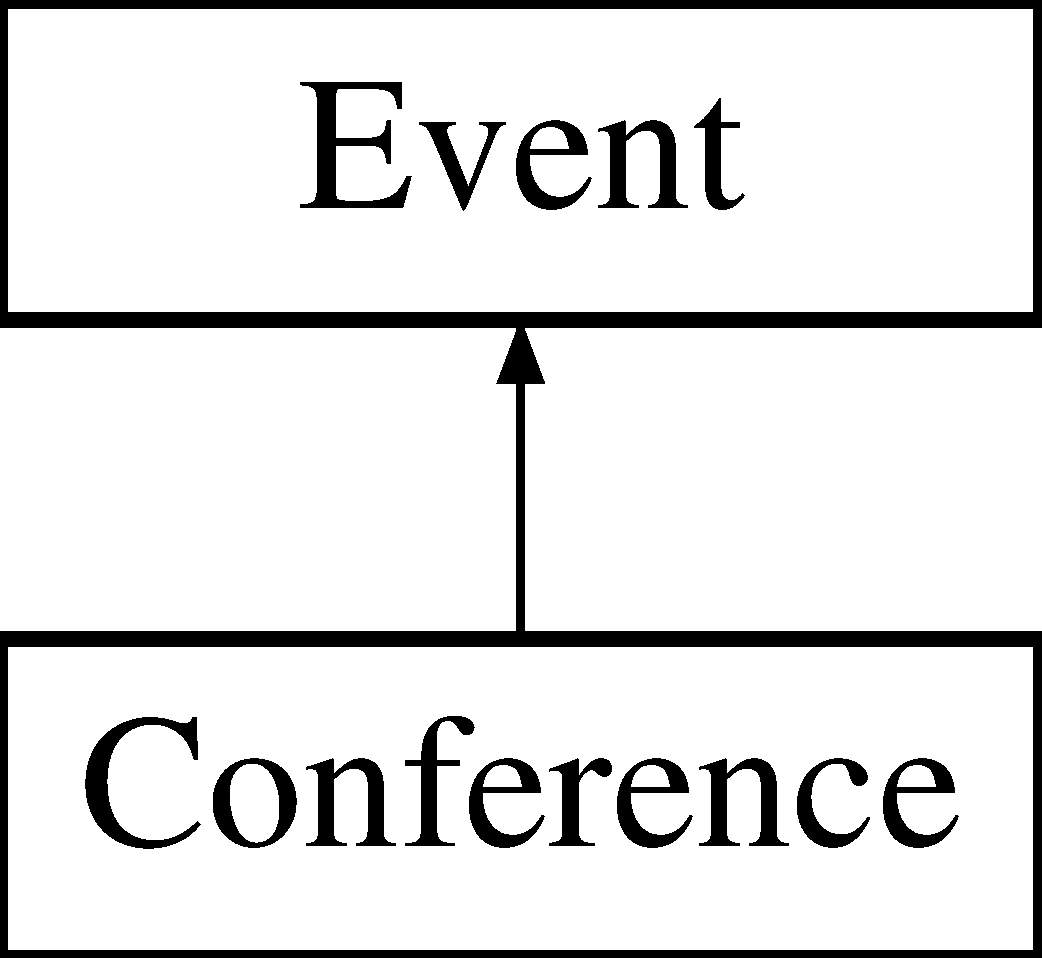
\includegraphics[height=2.000000cm]{classConference}
\end{center}
\end{figure}
\subsection*{Public Member Functions}
\begin{DoxyCompactItemize}
\item 
\mbox{\hyperlink{classConference_a433a85d640693398c2c96a2a655fc6f4}{Conference}} ()
\begin{DoxyCompactList}\small\item\em Default Constructor. \end{DoxyCompactList}\item 
\mbox{\hyperlink{classConference_a128ae6e184a018975429e6dda331c865}{Conference}} (std\+::vector$<$ \mbox{\hyperlink{classAssociate}{Associate}} $\ast$$>$ \mbox{\hyperlink{classEvent_a6cec387dca85f0a0e8419cfc94eb320e}{event\+\_\+request}}, std\+::vector$<$ \mbox{\hyperlink{classAssociate}{Associate}} $\ast$$>$ \mbox{\hyperlink{classEvent_ad35e04c759fdbfad75aed0b6e2eef63c}{event\+\_\+organizers}}, std\+::string \mbox{\hyperlink{classEvent_a9a93c9d38211f84cd6e347690e177f11}{date}}, std\+::string \mbox{\hyperlink{classEvent_a3d1f28a3bde9ab718d5b0003f8ab5129}{local}}, std\+::string \mbox{\hyperlink{classEvent_aa9cc4378d5cecaadc8e6de92b313e6f8}{theme}}, int \mbox{\hyperlink{classEvent_a4059db56458a92ddb5bd1d1443631b02}{phase}}, \mbox{\hyperlink{classAssociation}{Association}} $\ast$\mbox{\hyperlink{classEvent_a3c8694833e50dbd2e37943eff1f5c9b1}{association}}, int \mbox{\hyperlink{classConference_ab3acc9b9aec3a4dbcfd18d1611337ecb}{estimative}})
\begin{DoxyCompactList}\small\item\em Full \mbox{\hyperlink{classConference}{Conference}} Constructor. \end{DoxyCompactList}\item 
\mbox{\hyperlink{classConference_a576bd503bb7570120658b970223611c3}{Conference}} (std\+::vector$<$ \mbox{\hyperlink{classAssociate}{Associate}} $\ast$$>$ \mbox{\hyperlink{classEvent_a6cec387dca85f0a0e8419cfc94eb320e}{event\+\_\+request}}, std\+::vector$<$ \mbox{\hyperlink{classAssociate}{Associate}} $\ast$$>$ \mbox{\hyperlink{classEvent_ad35e04c759fdbfad75aed0b6e2eef63c}{event\+\_\+organizers}}, std\+::string \mbox{\hyperlink{classEvent_a9a93c9d38211f84cd6e347690e177f11}{date}}, std\+::string \mbox{\hyperlink{classEvent_a3d1f28a3bde9ab718d5b0003f8ab5129}{local}}, std\+::string \mbox{\hyperlink{classEvent_aa9cc4378d5cecaadc8e6de92b313e6f8}{theme}}, int \mbox{\hyperlink{classEvent_a4059db56458a92ddb5bd1d1443631b02}{phase}}, \mbox{\hyperlink{classAssociation}{Association}} $\ast$\mbox{\hyperlink{classEvent_a3c8694833e50dbd2e37943eff1f5c9b1}{association}}, int \mbox{\hyperlink{classConference_ab3acc9b9aec3a4dbcfd18d1611337ecb}{estimative}}, long double money)
\begin{DoxyCompactList}\small\item\em Full \mbox{\hyperlink{classConference}{Conference}} Constructor. \end{DoxyCompactList}\item 
virtual \mbox{\hyperlink{classConference_aad7fc5f411279abc70d4ff3c30d2bdd8}{$\sim$\+Conference}} ()
\begin{DoxyCompactList}\small\item\em Default \mbox{\hyperlink{classConference}{Conference}} Destructor. \end{DoxyCompactList}\item 
int \mbox{\hyperlink{classConference_a9d96f80eb37bdbf57bf318c8bd484e88}{get\+Estimative}} () const
\begin{DoxyCompactList}\small\item\em returns the number of people estimated to go to the conference \end{DoxyCompactList}\item 
std\+::string \mbox{\hyperlink{classConference_ad1cf07b29a4c4cc36483603ef9536186}{get\+Type}} () const
\begin{DoxyCompactList}\small\item\em returns the type of the event (\mbox{\hyperlink{classConference}{Conference}}) \end{DoxyCompactList}\item 
long double \mbox{\hyperlink{classConference_a6ca3f0f7b2714881dbc108ea7f08646f}{get\+Support}} () const
\begin{DoxyCompactList}\small\item\em returns the value of the monetary support given by the association \end{DoxyCompactList}\item 
std\+::list$<$ \mbox{\hyperlink{classTrainer}{Trainer}} $\ast$ $>$ \mbox{\hyperlink{classConference_aae9e92d48205a80fa42e94564e3568c5}{get\+Trainers}} () const
\begin{DoxyCompactList}\small\item\em returns the trainers who will attend the conference \end{DoxyCompactList}\item 
std\+::string \mbox{\hyperlink{classConference_a7a2f7b38c728f487d82356d3c671ef88}{show\+Info}} () const
\begin{DoxyCompactList}\small\item\em returns all the information about the conference \end{DoxyCompactList}\end{DoxyCompactItemize}
\subsection*{Private Attributes}
\begin{DoxyCompactItemize}
\item 
std\+::string \mbox{\hyperlink{classConference_af456d5097dc28808360f0d0fba2160c6}{type}} = \char`\"{}Conference\char`\"{}
\begin{DoxyCompactList}\small\item\em The type of the event. \end{DoxyCompactList}\item 
int \mbox{\hyperlink{classConference_ab3acc9b9aec3a4dbcfd18d1611337ecb}{estimative}}
\begin{DoxyCompactList}\small\item\em The number of people estimated to go to the conference. \end{DoxyCompactList}\item 
long double \mbox{\hyperlink{classConference_a800a31bff9c492bc417cf8cecf450195}{given\+\_\+support}}
\begin{DoxyCompactList}\small\item\em The value of the monetary support given by the association. \end{DoxyCompactList}\end{DoxyCompactItemize}
\subsection*{Additional Inherited Members}


\subsection{Detailed Description}
The \mbox{\hyperlink{classConference}{Conference}} Class -\/ Derived Class from the Super \mbox{\hyperlink{classEvent}{Event}} Class. 

A conference is a special type of event. This one has a estimative of people who will attend to the conference. 

\subsection{Constructor \& Destructor Documentation}
\mbox{\Hypertarget{classConference_a433a85d640693398c2c96a2a655fc6f4}\label{classConference_a433a85d640693398c2c96a2a655fc6f4}} 
\index{Conference@{Conference}!Conference@{Conference}}
\index{Conference@{Conference}!Conference@{Conference}}
\subsubsection{\texorpdfstring{Conference()}{Conference()}\hspace{0.1cm}{\footnotesize\ttfamily [1/3]}}
{\footnotesize\ttfamily Conference\+::\+Conference (\begin{DoxyParamCaption}{ }\end{DoxyParamCaption})}



Default Constructor. 

\mbox{\Hypertarget{classConference_a128ae6e184a018975429e6dda331c865}\label{classConference_a128ae6e184a018975429e6dda331c865}} 
\index{Conference@{Conference}!Conference@{Conference}}
\index{Conference@{Conference}!Conference@{Conference}}
\subsubsection{\texorpdfstring{Conference()}{Conference()}\hspace{0.1cm}{\footnotesize\ttfamily [2/3]}}
{\footnotesize\ttfamily Conference\+::\+Conference (\begin{DoxyParamCaption}\item[{std\+::vector$<$ \mbox{\hyperlink{classAssociate}{Associate}} $\ast$$>$}]{event\+\_\+request,  }\item[{std\+::vector$<$ \mbox{\hyperlink{classAssociate}{Associate}} $\ast$$>$}]{event\+\_\+organizers,  }\item[{std\+::string}]{date,  }\item[{std\+::string}]{local,  }\item[{std\+::string}]{theme,  }\item[{int}]{phase,  }\item[{\mbox{\hyperlink{classAssociation}{Association}} $\ast$}]{association,  }\item[{int}]{estimative }\end{DoxyParamCaption})}



Full \mbox{\hyperlink{classConference}{Conference}} Constructor. 


\begin{DoxyParams}{Parameters}
{\em event\+\_\+request} & -\/ The associates that requested the conference (up to 3) \\
\hline
{\em event\+\_\+organizers} & -\/ The associates that requested the conference (up to 3) and the ones who will help organize \\
\hline
{\em date} & -\/ The date of the conference \\
\hline
{\em local} & -\/ The local of the conference \\
\hline
{\em theme} & -\/ The theme of the conference \\
\hline
{\em phase} & -\/ The phase of the conference \\
\hline
{\em association} & -\/ The \mbox{\hyperlink{classAssociation}{Association}} that promotes the conference \\
\hline
{\em estimative} & -\/ The number of people estimated to go to the conference \\
\hline
\end{DoxyParams}
\mbox{\Hypertarget{classConference_a576bd503bb7570120658b970223611c3}\label{classConference_a576bd503bb7570120658b970223611c3}} 
\index{Conference@{Conference}!Conference@{Conference}}
\index{Conference@{Conference}!Conference@{Conference}}
\subsubsection{\texorpdfstring{Conference()}{Conference()}\hspace{0.1cm}{\footnotesize\ttfamily [3/3]}}
{\footnotesize\ttfamily Conference\+::\+Conference (\begin{DoxyParamCaption}\item[{std\+::vector$<$ \mbox{\hyperlink{classAssociate}{Associate}} $\ast$$>$}]{event\+\_\+request,  }\item[{std\+::vector$<$ \mbox{\hyperlink{classAssociate}{Associate}} $\ast$$>$}]{event\+\_\+organizers,  }\item[{std\+::string}]{date,  }\item[{std\+::string}]{local,  }\item[{std\+::string}]{theme,  }\item[{int}]{phase,  }\item[{\mbox{\hyperlink{classAssociation}{Association}} $\ast$}]{association,  }\item[{int}]{estimative,  }\item[{long double}]{money }\end{DoxyParamCaption})}



Full \mbox{\hyperlink{classConference}{Conference}} Constructor. 


\begin{DoxyParams}{Parameters}
{\em event\+\_\+request} & -\/ The associates that requested the conference (up to 3) \\
\hline
{\em event\+\_\+organizers} & -\/ The associates that requested the conference (up to 3) and the ones who will help organize \\
\hline
{\em date} & -\/ The date of the conference \\
\hline
{\em local} & -\/ The local of the conference \\
\hline
{\em theme} & -\/ The theme of the conference \\
\hline
{\em phase} & -\/ The phase of the conference \\
\hline
{\em association} & -\/ The \mbox{\hyperlink{classAssociation}{Association}} that promotes the conference \\
\hline
{\em estimative} & -\/ The number of people estimated to go to the conference \\
\hline
{\em money} & -\/ The amount the \mbox{\hyperlink{classAssociation}{Association}} gives to promote de event \\
\hline
\end{DoxyParams}
\mbox{\Hypertarget{classConference_aad7fc5f411279abc70d4ff3c30d2bdd8}\label{classConference_aad7fc5f411279abc70d4ff3c30d2bdd8}} 
\index{Conference@{Conference}!````~Conference@{$\sim$\+Conference}}
\index{````~Conference@{$\sim$\+Conference}!Conference@{Conference}}
\subsubsection{\texorpdfstring{$\sim$\+Conference()}{~Conference()}}
{\footnotesize\ttfamily Conference\+::$\sim$\+Conference (\begin{DoxyParamCaption}{ }\end{DoxyParamCaption})\hspace{0.3cm}{\ttfamily [virtual]}}



Default \mbox{\hyperlink{classConference}{Conference}} Destructor. 



\subsection{Member Function Documentation}
\mbox{\Hypertarget{classConference_a9d96f80eb37bdbf57bf318c8bd484e88}\label{classConference_a9d96f80eb37bdbf57bf318c8bd484e88}} 
\index{Conference@{Conference}!get\+Estimative@{get\+Estimative}}
\index{get\+Estimative@{get\+Estimative}!Conference@{Conference}}
\subsubsection{\texorpdfstring{get\+Estimative()}{getEstimative()}}
{\footnotesize\ttfamily int Conference\+::get\+Estimative (\begin{DoxyParamCaption}{ }\end{DoxyParamCaption}) const\hspace{0.3cm}{\ttfamily [virtual]}}



returns the number of people estimated to go to the conference 



Implements \mbox{\hyperlink{classEvent_a18ac55c239f648fc0ad5687c426f2a8f}{Event}}.

\mbox{\Hypertarget{classConference_a6ca3f0f7b2714881dbc108ea7f08646f}\label{classConference_a6ca3f0f7b2714881dbc108ea7f08646f}} 
\index{Conference@{Conference}!get\+Support@{get\+Support}}
\index{get\+Support@{get\+Support}!Conference@{Conference}}
\subsubsection{\texorpdfstring{get\+Support()}{getSupport()}}
{\footnotesize\ttfamily long double Conference\+::get\+Support (\begin{DoxyParamCaption}{ }\end{DoxyParamCaption}) const\hspace{0.3cm}{\ttfamily [virtual]}}



returns the value of the monetary support given by the association 



Implements \mbox{\hyperlink{classEvent_a9170bfcbd9b00015dafc5d5cc69a2cfe}{Event}}.

\mbox{\Hypertarget{classConference_aae9e92d48205a80fa42e94564e3568c5}\label{classConference_aae9e92d48205a80fa42e94564e3568c5}} 
\index{Conference@{Conference}!get\+Trainers@{get\+Trainers}}
\index{get\+Trainers@{get\+Trainers}!Conference@{Conference}}
\subsubsection{\texorpdfstring{get\+Trainers()}{getTrainers()}}
{\footnotesize\ttfamily list$<$ \mbox{\hyperlink{classTrainer}{Trainer}} $\ast$ $>$ Conference\+::get\+Trainers (\begin{DoxyParamCaption}{ }\end{DoxyParamCaption}) const\hspace{0.3cm}{\ttfamily [virtual]}}



returns the trainers who will attend the conference 



Implements \mbox{\hyperlink{classEvent_a11aad3e5a7ee85bc61b6811d050c5d70}{Event}}.

\mbox{\Hypertarget{classConference_ad1cf07b29a4c4cc36483603ef9536186}\label{classConference_ad1cf07b29a4c4cc36483603ef9536186}} 
\index{Conference@{Conference}!get\+Type@{get\+Type}}
\index{get\+Type@{get\+Type}!Conference@{Conference}}
\subsubsection{\texorpdfstring{get\+Type()}{getType()}}
{\footnotesize\ttfamily string Conference\+::get\+Type (\begin{DoxyParamCaption}{ }\end{DoxyParamCaption}) const\hspace{0.3cm}{\ttfamily [virtual]}}



returns the type of the event (\mbox{\hyperlink{classConference}{Conference}}) 



Implements \mbox{\hyperlink{classEvent_a224dbd9a9aee5937ba0c8ea1a056af1f}{Event}}.

\mbox{\Hypertarget{classConference_a7a2f7b38c728f487d82356d3c671ef88}\label{classConference_a7a2f7b38c728f487d82356d3c671ef88}} 
\index{Conference@{Conference}!show\+Info@{show\+Info}}
\index{show\+Info@{show\+Info}!Conference@{Conference}}
\subsubsection{\texorpdfstring{show\+Info()}{showInfo()}}
{\footnotesize\ttfamily string Conference\+::show\+Info (\begin{DoxyParamCaption}{ }\end{DoxyParamCaption}) const\hspace{0.3cm}{\ttfamily [virtual]}}



returns all the information about the conference 



Implements \mbox{\hyperlink{classEvent_aaa38f467e933c57190d43351bdb817be}{Event}}.



\subsection{Member Data Documentation}
\mbox{\Hypertarget{classConference_ab3acc9b9aec3a4dbcfd18d1611337ecb}\label{classConference_ab3acc9b9aec3a4dbcfd18d1611337ecb}} 
\index{Conference@{Conference}!estimative@{estimative}}
\index{estimative@{estimative}!Conference@{Conference}}
\subsubsection{\texorpdfstring{estimative}{estimative}}
{\footnotesize\ttfamily int Conference\+::estimative\hspace{0.3cm}{\ttfamily [private]}}



The number of people estimated to go to the conference. 

\mbox{\Hypertarget{classConference_a800a31bff9c492bc417cf8cecf450195}\label{classConference_a800a31bff9c492bc417cf8cecf450195}} 
\index{Conference@{Conference}!given\+\_\+support@{given\+\_\+support}}
\index{given\+\_\+support@{given\+\_\+support}!Conference@{Conference}}
\subsubsection{\texorpdfstring{given\+\_\+support}{given\_support}}
{\footnotesize\ttfamily long double Conference\+::given\+\_\+support\hspace{0.3cm}{\ttfamily [private]}}



The value of the monetary support given by the association. 

\mbox{\Hypertarget{classConference_af456d5097dc28808360f0d0fba2160c6}\label{classConference_af456d5097dc28808360f0d0fba2160c6}} 
\index{Conference@{Conference}!type@{type}}
\index{type@{type}!Conference@{Conference}}
\subsubsection{\texorpdfstring{type}{type}}
{\footnotesize\ttfamily std\+::string Conference\+::type = \char`\"{}Conference\char`\"{}\hspace{0.3cm}{\ttfamily [private]}}



The type of the event. 



The documentation for this class was generated from the following files\+:\begin{DoxyCompactItemize}
\item 
\mbox{\hyperlink{Conference_8h}{Conference.\+h}}\item 
\mbox{\hyperlink{Conference_8cpp}{Conference.\+cpp}}\end{DoxyCompactItemize}

\hypertarget{classEvent}{}\section{Event Class Reference}
\label{classEvent}\index{Event@{Event}}


The Super \mbox{\hyperlink{classEvent}{Event}} Class.  




{\ttfamily \#include $<$Event.\+h$>$}

Inheritance diagram for Event\+:\begin{figure}[H]
\begin{center}
\leavevmode
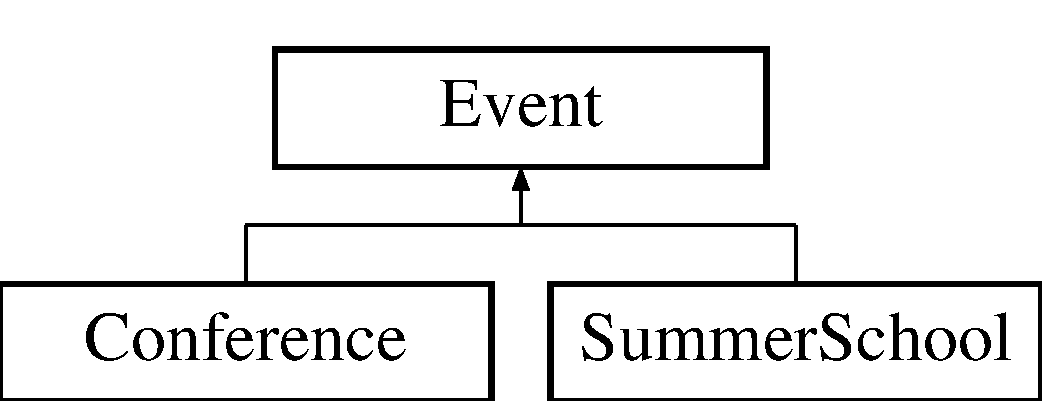
\includegraphics[height=2.000000cm]{classEvent}
\end{center}
\end{figure}
\subsection*{Public Member Functions}
\begin{DoxyCompactItemize}
\item 
\mbox{\hyperlink{classEvent_a5a40dd4708297f7031e29b39e039ae10}{Event}} ()
\begin{DoxyCompactList}\small\item\em Default Constructor. \end{DoxyCompactList}\item 
\mbox{\hyperlink{classEvent_a2fb2bff37e364023fe54d0f86e49e696}{Event}} (std\+::vector$<$ \mbox{\hyperlink{classAssociate}{Associate}} $\ast$$>$ \mbox{\hyperlink{classEvent_a6cec387dca85f0a0e8419cfc94eb320e}{event\+\_\+request}}, std\+::vector$<$ \mbox{\hyperlink{classAssociate}{Associate}} $\ast$$>$ \mbox{\hyperlink{classEvent_ad35e04c759fdbfad75aed0b6e2eef63c}{event\+\_\+organizers}}, std\+::string \mbox{\hyperlink{classEvent_a9a93c9d38211f84cd6e347690e177f11}{date}}, std\+::string \mbox{\hyperlink{classEvent_a3d1f28a3bde9ab718d5b0003f8ab5129}{local}}, std\+::string \mbox{\hyperlink{classEvent_aa9cc4378d5cecaadc8e6de92b313e6f8}{theme}}, int \mbox{\hyperlink{classEvent_a4059db56458a92ddb5bd1d1443631b02}{phase}}, \mbox{\hyperlink{classAssociation}{Association}} $\ast$\mbox{\hyperlink{classEvent_a3c8694833e50dbd2e37943eff1f5c9b1}{association}})
\begin{DoxyCompactList}\small\item\em Full \mbox{\hyperlink{classEvent}{Event}} Constructor The given support by the association will be any value between 5-\/15\% of the association main fund. \end{DoxyCompactList}\item 
virtual \mbox{\hyperlink{classEvent_a7704ec01ce91e673885792054214b3d2}{$\sim$\+Event}} ()
\begin{DoxyCompactList}\small\item\em Default \mbox{\hyperlink{classEvent}{Event}} Destructor. \end{DoxyCompactList}\item 
void \mbox{\hyperlink{classEvent_a21f01e4574335753b415d3445f1ebdff}{set\+Date}} (std\+::string \mbox{\hyperlink{classEvent_a9a93c9d38211f84cd6e347690e177f11}{date}})
\begin{DoxyCompactList}\small\item\em Sets/\+Changes the event\textquotesingle{}s date. \end{DoxyCompactList}\item 
void \mbox{\hyperlink{classEvent_ab4e1fd7cd5e56f58d3cd36a69e475054}{set\+Local}} (std\+::string \mbox{\hyperlink{classEvent_a3d1f28a3bde9ab718d5b0003f8ab5129}{local}})
\begin{DoxyCompactList}\small\item\em Sets/\+Changes the event\textquotesingle{}s local. \end{DoxyCompactList}\item 
void \mbox{\hyperlink{classEvent_abdd2c869f0231002c2a16813923586fb}{set\+Theme}} (std\+::string \mbox{\hyperlink{classEvent_aa9cc4378d5cecaadc8e6de92b313e6f8}{theme}})
\begin{DoxyCompactList}\small\item\em Sets/\+Changes the event\textquotesingle{}s theme. \end{DoxyCompactList}\item 
void \mbox{\hyperlink{classEvent_ab630975b378bad5230ae550b3e9ffc9a}{set\+Phase}} (int \mbox{\hyperlink{classEvent_a4059db56458a92ddb5bd1d1443631b02}{phase}})
\begin{DoxyCompactList}\small\item\em Sets/\+Changes the event\textquotesingle{}s phase. \end{DoxyCompactList}\item 
std\+::vector$<$ \mbox{\hyperlink{classAssociate}{Associate}} $\ast$ $>$ \mbox{\hyperlink{classEvent_a424a2862591a8437b0d18366c7aee247}{get\+Request}} () const
\begin{DoxyCompactList}\small\item\em Returns the associates that gave the initial request to the event. \end{DoxyCompactList}\item 
std\+::vector$<$ \mbox{\hyperlink{classAssociate}{Associate}} $\ast$ $>$ \mbox{\hyperlink{classEvent_a7e09dd7707422e30104727a069573e88}{get\+Organizers}} () const
\begin{DoxyCompactList}\small\item\em Returns all the associates that are involved in the event. \end{DoxyCompactList}\item 
std\+::string \mbox{\hyperlink{classEvent_a42abbf59c83e3fa6c964463a5e65ea00}{get\+Date}} () const
\begin{DoxyCompactList}\small\item\em Returns the Date of the event. \end{DoxyCompactList}\item 
std\+::string \mbox{\hyperlink{classEvent_aa2b3aee8416f68b890083a09eecfea8b}{get\+Local}} () const
\begin{DoxyCompactList}\small\item\em Returns the Local of the event. \end{DoxyCompactList}\item 
std\+::string \mbox{\hyperlink{classEvent_ad83e88dd2fe78a6840dd2c71d217b490}{get\+Theme}} () const
\begin{DoxyCompactList}\small\item\em Returns the Theme of the event. \end{DoxyCompactList}\item 
int \mbox{\hyperlink{classEvent_a1f6eac3425718082f5445a46a236b837}{get\+Phase}} () const
\begin{DoxyCompactList}\small\item\em Returns the Phase of the event. \end{DoxyCompactList}\item 
virtual long double \mbox{\hyperlink{classEvent_a9170bfcbd9b00015dafc5d5cc69a2cfe}{get\+Support}} () const =0
\begin{DoxyCompactList}\small\item\em Returns the value of the monetary support given by the association to the e event. \end{DoxyCompactList}\item 
virtual std\+::string \mbox{\hyperlink{classEvent_a224dbd9a9aee5937ba0c8ea1a056af1f}{get\+Type}} () const =0
\begin{DoxyCompactList}\small\item\em Returns the Type of the event. \end{DoxyCompactList}\item 
virtual std\+::list$<$ \mbox{\hyperlink{classTrainer}{Trainer}} $\ast$ $>$ \mbox{\hyperlink{classEvent_a11aad3e5a7ee85bc61b6811d050c5d70}{get\+Trainers}} () const =0
\begin{DoxyCompactList}\small\item\em Returns the trainers that will attend the event. \end{DoxyCompactList}\item 
virtual int \mbox{\hyperlink{classEvent_a18ac55c239f648fc0ad5687c426f2a8f}{get\+Estimative}} () const =0
\begin{DoxyCompactList}\small\item\em Returns the estimative of the people who will attend the event. \end{DoxyCompactList}\item 
virtual std\+::string \mbox{\hyperlink{classEvent_aaa38f467e933c57190d43351bdb817be}{show\+Info}} () const =0
\begin{DoxyCompactList}\small\item\em Returns all the information of the event. \end{DoxyCompactList}\item 
std\+::string \mbox{\hyperlink{classEvent_a36453ab5a21b660a61f2a0369e2689e8}{get\+Name}} () const
\begin{DoxyCompactList}\small\item\em Returns the name of the event. \end{DoxyCompactList}\item 
bool \mbox{\hyperlink{classEvent_a9a62a5f6528c63c84c30fa9edd50ddb1}{operator$<$}} (\mbox{\hyperlink{classEvent}{Event}} $\ast$ev1) const
\begin{DoxyCompactList}\small\item\em operator for both priority queues \end{DoxyCompactList}\end{DoxyCompactItemize}
\subsection*{Protected Attributes}
\begin{DoxyCompactItemize}
\item 
std\+::vector$<$ \mbox{\hyperlink{classAssociate}{Associate}} $\ast$ $>$ \mbox{\hyperlink{classEvent_a6cec387dca85f0a0e8419cfc94eb320e}{event\+\_\+request}}
\begin{DoxyCompactList}\small\item\em The Associates that gave the initial request. \end{DoxyCompactList}\item 
std\+::vector$<$ \mbox{\hyperlink{classAssociate}{Associate}} $\ast$ $>$ \mbox{\hyperlink{classEvent_ad35e04c759fdbfad75aed0b6e2eef63c}{event\+\_\+organizers}}
\begin{DoxyCompactList}\small\item\em All the associates involved with the event. \end{DoxyCompactList}\item 
std\+::string \mbox{\hyperlink{classEvent_a9a93c9d38211f84cd6e347690e177f11}{date}}
\begin{DoxyCompactList}\small\item\em The event\textquotesingle{}s date. \end{DoxyCompactList}\item 
std\+::string \mbox{\hyperlink{classEvent_a3d1f28a3bde9ab718d5b0003f8ab5129}{local}}
\begin{DoxyCompactList}\small\item\em The event\textquotesingle{}s local. \end{DoxyCompactList}\item 
std\+::string \mbox{\hyperlink{classEvent_aa9cc4378d5cecaadc8e6de92b313e6f8}{theme}}
\begin{DoxyCompactList}\small\item\em The event\textquotesingle{}s theme. \end{DoxyCompactList}\item 
int \mbox{\hyperlink{classEvent_a4059db56458a92ddb5bd1d1443631b02}{phase}}
\begin{DoxyCompactList}\small\item\em The event\textquotesingle{}s phase. \end{DoxyCompactList}\item 
\mbox{\hyperlink{classAssociation}{Association}} $\ast$ \mbox{\hyperlink{classEvent_a3c8694833e50dbd2e37943eff1f5c9b1}{association}}
\begin{DoxyCompactList}\small\item\em The connection to the \mbox{\hyperlink{classAssociation}{Association}}. \end{DoxyCompactList}\end{DoxyCompactItemize}


\subsection{Detailed Description}
The Super \mbox{\hyperlink{classEvent}{Event}} Class. 

An \mbox{\hyperlink{classEvent}{Event}} must be requested by at least 3 Associates. The given monetary support given by the association is determined randomly, taking in consideration the association main fund. In this case, we chose to give it a value between 5-\/15\% of the total Fund; This given monetary support will be later used to calculate the total number of organizers (then selected randomly between all the associates) and trainers. 

\subsection{Constructor \& Destructor Documentation}
\mbox{\Hypertarget{classEvent_a5a40dd4708297f7031e29b39e039ae10}\label{classEvent_a5a40dd4708297f7031e29b39e039ae10}} 
\index{Event@{Event}!Event@{Event}}
\index{Event@{Event}!Event@{Event}}
\subsubsection{\texorpdfstring{Event()}{Event()}\hspace{0.1cm}{\footnotesize\ttfamily [1/2]}}
{\footnotesize\ttfamily Event\+::\+Event (\begin{DoxyParamCaption}{ }\end{DoxyParamCaption})}



Default Constructor. 

\mbox{\Hypertarget{classEvent_a2fb2bff37e364023fe54d0f86e49e696}\label{classEvent_a2fb2bff37e364023fe54d0f86e49e696}} 
\index{Event@{Event}!Event@{Event}}
\index{Event@{Event}!Event@{Event}}
\subsubsection{\texorpdfstring{Event()}{Event()}\hspace{0.1cm}{\footnotesize\ttfamily [2/2]}}
{\footnotesize\ttfamily Event\+::\+Event (\begin{DoxyParamCaption}\item[{std\+::vector$<$ \mbox{\hyperlink{classAssociate}{Associate}} $\ast$$>$}]{event\+\_\+request,  }\item[{std\+::vector$<$ \mbox{\hyperlink{classAssociate}{Associate}} $\ast$$>$}]{event\+\_\+organizers,  }\item[{std\+::string}]{date,  }\item[{std\+::string}]{local,  }\item[{std\+::string}]{theme,  }\item[{int}]{phase,  }\item[{\mbox{\hyperlink{classAssociation}{Association}} $\ast$}]{association }\end{DoxyParamCaption})}



Full \mbox{\hyperlink{classEvent}{Event}} Constructor The given support by the association will be any value between 5-\/15\% of the association main fund. 


\begin{DoxyParams}{Parameters}
{\em event\+\_\+request} & -\/ The associates that requested the event (up to 3) \\
\hline
{\em event\+\_\+organizers} & -\/ The associates that requested the event (up to 3) and the ones who will help organize \\
\hline
{\em date} & -\/ The date of the event \\
\hline
{\em local} & -\/ The local of the event \\
\hline
{\em theme} & -\/ The theme of the event \\
\hline
{\em association} & -\/ The \mbox{\hyperlink{classAssociation}{Association}} that promotes the event \\
\hline
\end{DoxyParams}
\mbox{\Hypertarget{classEvent_a7704ec01ce91e673885792054214b3d2}\label{classEvent_a7704ec01ce91e673885792054214b3d2}} 
\index{Event@{Event}!````~Event@{$\sim$\+Event}}
\index{````~Event@{$\sim$\+Event}!Event@{Event}}
\subsubsection{\texorpdfstring{$\sim$\+Event()}{~Event()}}
{\footnotesize\ttfamily Event\+::$\sim$\+Event (\begin{DoxyParamCaption}{ }\end{DoxyParamCaption})\hspace{0.3cm}{\ttfamily [virtual]}}



Default \mbox{\hyperlink{classEvent}{Event}} Destructor. 



\subsection{Member Function Documentation}
\mbox{\Hypertarget{classEvent_a42abbf59c83e3fa6c964463a5e65ea00}\label{classEvent_a42abbf59c83e3fa6c964463a5e65ea00}} 
\index{Event@{Event}!get\+Date@{get\+Date}}
\index{get\+Date@{get\+Date}!Event@{Event}}
\subsubsection{\texorpdfstring{get\+Date()}{getDate()}}
{\footnotesize\ttfamily string Event\+::get\+Date (\begin{DoxyParamCaption}{ }\end{DoxyParamCaption}) const}



Returns the Date of the event. 

\mbox{\Hypertarget{classEvent_a18ac55c239f648fc0ad5687c426f2a8f}\label{classEvent_a18ac55c239f648fc0ad5687c426f2a8f}} 
\index{Event@{Event}!get\+Estimative@{get\+Estimative}}
\index{get\+Estimative@{get\+Estimative}!Event@{Event}}
\subsubsection{\texorpdfstring{get\+Estimative()}{getEstimative()}}
{\footnotesize\ttfamily virtual int Event\+::get\+Estimative (\begin{DoxyParamCaption}{ }\end{DoxyParamCaption}) const\hspace{0.3cm}{\ttfamily [pure virtual]}}



Returns the estimative of the people who will attend the event. 



Implemented in \mbox{\hyperlink{classSummerSchool_a019b9e38108b7dd31cd93cab285d0d00}{Summer\+School}}, and \mbox{\hyperlink{classConference_a9d96f80eb37bdbf57bf318c8bd484e88}{Conference}}.

\mbox{\Hypertarget{classEvent_aa2b3aee8416f68b890083a09eecfea8b}\label{classEvent_aa2b3aee8416f68b890083a09eecfea8b}} 
\index{Event@{Event}!get\+Local@{get\+Local}}
\index{get\+Local@{get\+Local}!Event@{Event}}
\subsubsection{\texorpdfstring{get\+Local()}{getLocal()}}
{\footnotesize\ttfamily string Event\+::get\+Local (\begin{DoxyParamCaption}{ }\end{DoxyParamCaption}) const}



Returns the Local of the event. 

\mbox{\Hypertarget{classEvent_a36453ab5a21b660a61f2a0369e2689e8}\label{classEvent_a36453ab5a21b660a61f2a0369e2689e8}} 
\index{Event@{Event}!get\+Name@{get\+Name}}
\index{get\+Name@{get\+Name}!Event@{Event}}
\subsubsection{\texorpdfstring{get\+Name()}{getName()}}
{\footnotesize\ttfamily std\+::string Event\+::get\+Name (\begin{DoxyParamCaption}{ }\end{DoxyParamCaption}) const\hspace{0.3cm}{\ttfamily [inline]}}



Returns the name of the event. 

\mbox{\Hypertarget{classEvent_a7e09dd7707422e30104727a069573e88}\label{classEvent_a7e09dd7707422e30104727a069573e88}} 
\index{Event@{Event}!get\+Organizers@{get\+Organizers}}
\index{get\+Organizers@{get\+Organizers}!Event@{Event}}
\subsubsection{\texorpdfstring{get\+Organizers()}{getOrganizers()}}
{\footnotesize\ttfamily vector$<$ \mbox{\hyperlink{classAssociate}{Associate}} $\ast$ $>$ Event\+::get\+Organizers (\begin{DoxyParamCaption}{ }\end{DoxyParamCaption}) const}



Returns all the associates that are involved in the event. 

\mbox{\Hypertarget{classEvent_a1f6eac3425718082f5445a46a236b837}\label{classEvent_a1f6eac3425718082f5445a46a236b837}} 
\index{Event@{Event}!get\+Phase@{get\+Phase}}
\index{get\+Phase@{get\+Phase}!Event@{Event}}
\subsubsection{\texorpdfstring{get\+Phase()}{getPhase()}}
{\footnotesize\ttfamily int Event\+::get\+Phase (\begin{DoxyParamCaption}{ }\end{DoxyParamCaption}) const}



Returns the Phase of the event. 

\mbox{\Hypertarget{classEvent_a424a2862591a8437b0d18366c7aee247}\label{classEvent_a424a2862591a8437b0d18366c7aee247}} 
\index{Event@{Event}!get\+Request@{get\+Request}}
\index{get\+Request@{get\+Request}!Event@{Event}}
\subsubsection{\texorpdfstring{get\+Request()}{getRequest()}}
{\footnotesize\ttfamily vector$<$ \mbox{\hyperlink{classAssociate}{Associate}} $\ast$ $>$ Event\+::get\+Request (\begin{DoxyParamCaption}{ }\end{DoxyParamCaption}) const}



Returns the associates that gave the initial request to the event. 

\mbox{\Hypertarget{classEvent_a9170bfcbd9b00015dafc5d5cc69a2cfe}\label{classEvent_a9170bfcbd9b00015dafc5d5cc69a2cfe}} 
\index{Event@{Event}!get\+Support@{get\+Support}}
\index{get\+Support@{get\+Support}!Event@{Event}}
\subsubsection{\texorpdfstring{get\+Support()}{getSupport()}}
{\footnotesize\ttfamily virtual long double Event\+::get\+Support (\begin{DoxyParamCaption}{ }\end{DoxyParamCaption}) const\hspace{0.3cm}{\ttfamily [pure virtual]}}



Returns the value of the monetary support given by the association to the e event. 



Implemented in \mbox{\hyperlink{classSummerSchool_a86f34a2f39dcd33171e77c386165219c}{Summer\+School}}, and \mbox{\hyperlink{classConference_a6ca3f0f7b2714881dbc108ea7f08646f}{Conference}}.

\mbox{\Hypertarget{classEvent_ad83e88dd2fe78a6840dd2c71d217b490}\label{classEvent_ad83e88dd2fe78a6840dd2c71d217b490}} 
\index{Event@{Event}!get\+Theme@{get\+Theme}}
\index{get\+Theme@{get\+Theme}!Event@{Event}}
\subsubsection{\texorpdfstring{get\+Theme()}{getTheme()}}
{\footnotesize\ttfamily string Event\+::get\+Theme (\begin{DoxyParamCaption}{ }\end{DoxyParamCaption}) const}



Returns the Theme of the event. 

\mbox{\Hypertarget{classEvent_a11aad3e5a7ee85bc61b6811d050c5d70}\label{classEvent_a11aad3e5a7ee85bc61b6811d050c5d70}} 
\index{Event@{Event}!get\+Trainers@{get\+Trainers}}
\index{get\+Trainers@{get\+Trainers}!Event@{Event}}
\subsubsection{\texorpdfstring{get\+Trainers()}{getTrainers()}}
{\footnotesize\ttfamily virtual std\+::list$<$\mbox{\hyperlink{classTrainer}{Trainer}} $\ast$$>$ Event\+::get\+Trainers (\begin{DoxyParamCaption}{ }\end{DoxyParamCaption}) const\hspace{0.3cm}{\ttfamily [pure virtual]}}



Returns the trainers that will attend the event. 



Implemented in \mbox{\hyperlink{classSummerSchool_aba18410ee9fbafd26858232104b5b39f}{Summer\+School}}, and \mbox{\hyperlink{classConference_aae9e92d48205a80fa42e94564e3568c5}{Conference}}.

\mbox{\Hypertarget{classEvent_a224dbd9a9aee5937ba0c8ea1a056af1f}\label{classEvent_a224dbd9a9aee5937ba0c8ea1a056af1f}} 
\index{Event@{Event}!get\+Type@{get\+Type}}
\index{get\+Type@{get\+Type}!Event@{Event}}
\subsubsection{\texorpdfstring{get\+Type()}{getType()}}
{\footnotesize\ttfamily virtual std\+::string Event\+::get\+Type (\begin{DoxyParamCaption}{ }\end{DoxyParamCaption}) const\hspace{0.3cm}{\ttfamily [pure virtual]}}



Returns the Type of the event. 



Implemented in \mbox{\hyperlink{classSummerSchool_a2ba547411ca8f161c2c579f9f55f913e}{Summer\+School}}, and \mbox{\hyperlink{classConference_ad1cf07b29a4c4cc36483603ef9536186}{Conference}}.

\mbox{\Hypertarget{classEvent_a9a62a5f6528c63c84c30fa9edd50ddb1}\label{classEvent_a9a62a5f6528c63c84c30fa9edd50ddb1}} 
\index{Event@{Event}!operator$<$@{operator$<$}}
\index{operator$<$@{operator$<$}!Event@{Event}}
\subsubsection{\texorpdfstring{operator$<$()}{operator<()}}
{\footnotesize\ttfamily bool Event\+::operator$<$ (\begin{DoxyParamCaption}\item[{\mbox{\hyperlink{classEvent}{Event}} $\ast$}]{ev1 }\end{DoxyParamCaption}) const}



operator for both priority queues 


\begin{DoxyParams}{Parameters}
{\em ev1} & -\/ \mbox{\hyperlink{classEvent}{Event}} to be compared \\
\hline
\end{DoxyParams}
\mbox{\Hypertarget{classEvent_a21f01e4574335753b415d3445f1ebdff}\label{classEvent_a21f01e4574335753b415d3445f1ebdff}} 
\index{Event@{Event}!set\+Date@{set\+Date}}
\index{set\+Date@{set\+Date}!Event@{Event}}
\subsubsection{\texorpdfstring{set\+Date()}{setDate()}}
{\footnotesize\ttfamily void Event\+::set\+Date (\begin{DoxyParamCaption}\item[{std\+::string}]{date }\end{DoxyParamCaption})}



Sets/\+Changes the event\textquotesingle{}s date. 


\begin{DoxyParams}{Parameters}
{\em date} & -\/ The new event\textquotesingle{}s date \\
\hline
\end{DoxyParams}
\mbox{\Hypertarget{classEvent_ab4e1fd7cd5e56f58d3cd36a69e475054}\label{classEvent_ab4e1fd7cd5e56f58d3cd36a69e475054}} 
\index{Event@{Event}!set\+Local@{set\+Local}}
\index{set\+Local@{set\+Local}!Event@{Event}}
\subsubsection{\texorpdfstring{set\+Local()}{setLocal()}}
{\footnotesize\ttfamily void Event\+::set\+Local (\begin{DoxyParamCaption}\item[{std\+::string}]{local }\end{DoxyParamCaption})}



Sets/\+Changes the event\textquotesingle{}s local. 


\begin{DoxyParams}{Parameters}
{\em local} & -\/ The new event\textquotesingle{}s local \\
\hline
\end{DoxyParams}
\mbox{\Hypertarget{classEvent_ab630975b378bad5230ae550b3e9ffc9a}\label{classEvent_ab630975b378bad5230ae550b3e9ffc9a}} 
\index{Event@{Event}!set\+Phase@{set\+Phase}}
\index{set\+Phase@{set\+Phase}!Event@{Event}}
\subsubsection{\texorpdfstring{set\+Phase()}{setPhase()}}
{\footnotesize\ttfamily void Event\+::set\+Phase (\begin{DoxyParamCaption}\item[{int}]{phase }\end{DoxyParamCaption})}



Sets/\+Changes the event\textquotesingle{}s phase. 


\begin{DoxyParams}{Parameters}
{\em theme} & -\/ The new event\textquotesingle{}s phase \\
\hline
\end{DoxyParams}
\mbox{\Hypertarget{classEvent_abdd2c869f0231002c2a16813923586fb}\label{classEvent_abdd2c869f0231002c2a16813923586fb}} 
\index{Event@{Event}!set\+Theme@{set\+Theme}}
\index{set\+Theme@{set\+Theme}!Event@{Event}}
\subsubsection{\texorpdfstring{set\+Theme()}{setTheme()}}
{\footnotesize\ttfamily void Event\+::set\+Theme (\begin{DoxyParamCaption}\item[{std\+::string}]{theme }\end{DoxyParamCaption})}



Sets/\+Changes the event\textquotesingle{}s theme. 


\begin{DoxyParams}{Parameters}
{\em theme} & -\/ The new event\textquotesingle{}s theme \\
\hline
\end{DoxyParams}
\mbox{\Hypertarget{classEvent_aaa38f467e933c57190d43351bdb817be}\label{classEvent_aaa38f467e933c57190d43351bdb817be}} 
\index{Event@{Event}!show\+Info@{show\+Info}}
\index{show\+Info@{show\+Info}!Event@{Event}}
\subsubsection{\texorpdfstring{show\+Info()}{showInfo()}}
{\footnotesize\ttfamily virtual std\+::string Event\+::show\+Info (\begin{DoxyParamCaption}{ }\end{DoxyParamCaption}) const\hspace{0.3cm}{\ttfamily [pure virtual]}}



Returns all the information of the event. 



Implemented in \mbox{\hyperlink{classSummerSchool_a61ac7307840f787e3de639d431248e26}{Summer\+School}}, and \mbox{\hyperlink{classConference_a7a2f7b38c728f487d82356d3c671ef88}{Conference}}.



\subsection{Member Data Documentation}
\mbox{\Hypertarget{classEvent_a3c8694833e50dbd2e37943eff1f5c9b1}\label{classEvent_a3c8694833e50dbd2e37943eff1f5c9b1}} 
\index{Event@{Event}!association@{association}}
\index{association@{association}!Event@{Event}}
\subsubsection{\texorpdfstring{association}{association}}
{\footnotesize\ttfamily \mbox{\hyperlink{classAssociation}{Association}}$\ast$ Event\+::association\hspace{0.3cm}{\ttfamily [protected]}}



The connection to the \mbox{\hyperlink{classAssociation}{Association}}. 

\mbox{\Hypertarget{classEvent_a9a93c9d38211f84cd6e347690e177f11}\label{classEvent_a9a93c9d38211f84cd6e347690e177f11}} 
\index{Event@{Event}!date@{date}}
\index{date@{date}!Event@{Event}}
\subsubsection{\texorpdfstring{date}{date}}
{\footnotesize\ttfamily std\+::string Event\+::date\hspace{0.3cm}{\ttfamily [protected]}}



The event\textquotesingle{}s date. 

\mbox{\Hypertarget{classEvent_ad35e04c759fdbfad75aed0b6e2eef63c}\label{classEvent_ad35e04c759fdbfad75aed0b6e2eef63c}} 
\index{Event@{Event}!event\+\_\+organizers@{event\+\_\+organizers}}
\index{event\+\_\+organizers@{event\+\_\+organizers}!Event@{Event}}
\subsubsection{\texorpdfstring{event\+\_\+organizers}{event\_organizers}}
{\footnotesize\ttfamily std\+::vector$<$\mbox{\hyperlink{classAssociate}{Associate}} $\ast$$>$ Event\+::event\+\_\+organizers\hspace{0.3cm}{\ttfamily [protected]}}



All the associates involved with the event. 

\mbox{\Hypertarget{classEvent_a6cec387dca85f0a0e8419cfc94eb320e}\label{classEvent_a6cec387dca85f0a0e8419cfc94eb320e}} 
\index{Event@{Event}!event\+\_\+request@{event\+\_\+request}}
\index{event\+\_\+request@{event\+\_\+request}!Event@{Event}}
\subsubsection{\texorpdfstring{event\+\_\+request}{event\_request}}
{\footnotesize\ttfamily std\+::vector$<$\mbox{\hyperlink{classAssociate}{Associate}} $\ast$$>$ Event\+::event\+\_\+request\hspace{0.3cm}{\ttfamily [protected]}}



The Associates that gave the initial request. 

\mbox{\Hypertarget{classEvent_a3d1f28a3bde9ab718d5b0003f8ab5129}\label{classEvent_a3d1f28a3bde9ab718d5b0003f8ab5129}} 
\index{Event@{Event}!local@{local}}
\index{local@{local}!Event@{Event}}
\subsubsection{\texorpdfstring{local}{local}}
{\footnotesize\ttfamily std\+::string Event\+::local\hspace{0.3cm}{\ttfamily [protected]}}



The event\textquotesingle{}s local. 

\mbox{\Hypertarget{classEvent_a4059db56458a92ddb5bd1d1443631b02}\label{classEvent_a4059db56458a92ddb5bd1d1443631b02}} 
\index{Event@{Event}!phase@{phase}}
\index{phase@{phase}!Event@{Event}}
\subsubsection{\texorpdfstring{phase}{phase}}
{\footnotesize\ttfamily int Event\+::phase\hspace{0.3cm}{\ttfamily [protected]}}



The event\textquotesingle{}s phase. 

\mbox{\Hypertarget{classEvent_aa9cc4378d5cecaadc8e6de92b313e6f8}\label{classEvent_aa9cc4378d5cecaadc8e6de92b313e6f8}} 
\index{Event@{Event}!theme@{theme}}
\index{theme@{theme}!Event@{Event}}
\subsubsection{\texorpdfstring{theme}{theme}}
{\footnotesize\ttfamily std\+::string Event\+::theme\hspace{0.3cm}{\ttfamily [protected]}}



The event\textquotesingle{}s theme. 



The documentation for this class was generated from the following files\+:\begin{DoxyCompactItemize}
\item 
\mbox{\hyperlink{Event_8h}{Event.\+h}}\item 
\mbox{\hyperlink{Event_8cpp}{Event.\+cpp}}\end{DoxyCompactItemize}

\hypertarget{classMail}{}\section{Mail Class Reference}
\label{classMail}\index{Mail@{Mail}}


The \hyperlink{classMail}{Mail} Class.  




{\ttfamily \#include $<$Mail.\+h$>$}

\subsection*{Public Member Functions}
\begin{DoxyCompactItemize}
\item 
\hyperlink{classMail_acd3d916cd6a769cdaf6e91dbc2c85699}{Mail} ()
\begin{DoxyCompactList}\small\item\em Default Constructor. \end{DoxyCompactList}\item 
\hyperlink{classMail_a5801c10c9e03a2ea2f0def9f5a957e18}{Mail} (\hyperlink{classAssociate}{Associate} $\ast$associate, std\+::string \hyperlink{classMail_a2f54f71a529dec6345d84ae60562b207}{title}, std\+::string \hyperlink{classMail_aaa91a94ee92b2712218a9cae389554f7}{body}, std\+::string \hyperlink{classMail_aee9bc87682f6173b92bf135397f38162}{date})
\begin{DoxyCompactList}\small\item\em Creates a new mail from the associate with a title and a body. \end{DoxyCompactList}\item 
virtual \hyperlink{classMail_a7f59d642ff71033500e1fac06ce9b3b1}{$\sim$\+Mail} ()
\begin{DoxyCompactList}\small\item\em Default Destructor. \end{DoxyCompactList}\item 
\hyperlink{classAssociate}{Associate} $\ast$ \hyperlink{classMail_a23db9880d8a7d0fed31668b895fc3899}{get\+Author} () const
\begin{DoxyCompactList}\small\item\em Returns the author from the mail. \end{DoxyCompactList}\item 
std\+::string \hyperlink{classMail_aa51a6657dd3e594e8638ac4486660675}{get\+Title} () const
\begin{DoxyCompactList}\small\item\em Returns the mail title. \end{DoxyCompactList}\item 
std\+::string \hyperlink{classMail_af89b1b3d0f3c9d92a272c06f18fbdec3}{get\+Body} () const
\begin{DoxyCompactList}\small\item\em Returns the mail body. \end{DoxyCompactList}\item 
std\+::string \hyperlink{classMail_ac45841e601864ec3f84566c3ee77de9a}{get\+Date} () const
\begin{DoxyCompactList}\small\item\em Returns the mail date. \end{DoxyCompactList}\item 
void \hyperlink{classMail_acec00cbed8830746de97efeca4561dd8}{set\+Author} (\hyperlink{classAssociate}{Associate} $\ast$\hyperlink{classMail_acfe110a866f8cc54120d4f4ab0f8321b}{author})
\begin{DoxyCompactList}\small\item\em Sets/\+Changes the author from a mail. \end{DoxyCompactList}\item 
void \hyperlink{classMail_aa57f6b5a2f81ded349476984c361275b}{set\+Title} (std\+::string \hyperlink{classMail_a2f54f71a529dec6345d84ae60562b207}{title})
\begin{DoxyCompactList}\small\item\em Sets/\+Changes the title from a mail. \end{DoxyCompactList}\item 
void \hyperlink{classMail_a85ddf08af27648cc0835d66bd6b08dde}{set\+Body} (std\+::string \hyperlink{classMail_aaa91a94ee92b2712218a9cae389554f7}{body})
\begin{DoxyCompactList}\small\item\em Sets/\+Changes the body from a mail. \end{DoxyCompactList}\item 
void \hyperlink{classMail_ac5c8d190278b895b2de786be431b0a30}{set\+Date} (std\+::string \hyperlink{classMail_aee9bc87682f6173b92bf135397f38162}{date})
\begin{DoxyCompactList}\small\item\em Sets/\+Changes the date from a mail. \end{DoxyCompactList}\end{DoxyCompactItemize}
\subsection*{Private Attributes}
\begin{DoxyCompactItemize}
\item 
\hyperlink{classAssociate}{Associate} $\ast$ \hyperlink{classMail_acfe110a866f8cc54120d4f4ab0f8321b}{author}
\begin{DoxyCompactList}\small\item\em The mail\textquotesingle{}s author. \end{DoxyCompactList}\item 
std\+::string \hyperlink{classMail_a2f54f71a529dec6345d84ae60562b207}{title}
\begin{DoxyCompactList}\small\item\em The mail\textquotesingle{}s title. \end{DoxyCompactList}\item 
std\+::string \hyperlink{classMail_aaa91a94ee92b2712218a9cae389554f7}{body}
\begin{DoxyCompactList}\small\item\em The mail\textquotesingle{}s body. \end{DoxyCompactList}\item 
std\+::string \hyperlink{classMail_aee9bc87682f6173b92bf135397f38162}{date}
\begin{DoxyCompactList}\small\item\em The mail\textquotesingle{}s date. \end{DoxyCompactList}\end{DoxyCompactItemize}


\subsection{Detailed Description}
The \hyperlink{classMail}{Mail} Class. 

The \hyperlink{classNetwork}{Network} is used by the associates to send and receive mails. So, each mail will have an author, a title, the body of the mail and a data associated with it. 

\subsection{Constructor \& Destructor Documentation}
\mbox{\Hypertarget{classMail_acd3d916cd6a769cdaf6e91dbc2c85699}\label{classMail_acd3d916cd6a769cdaf6e91dbc2c85699}} 
\index{Mail@{Mail}!Mail@{Mail}}
\index{Mail@{Mail}!Mail@{Mail}}
\subsubsection{\texorpdfstring{Mail()}{Mail()}\hspace{0.1cm}{\footnotesize\ttfamily [1/2]}}
{\footnotesize\ttfamily Mail\+::\+Mail (\begin{DoxyParamCaption}{ }\end{DoxyParamCaption})}



Default Constructor. 

\mbox{\Hypertarget{classMail_a5801c10c9e03a2ea2f0def9f5a957e18}\label{classMail_a5801c10c9e03a2ea2f0def9f5a957e18}} 
\index{Mail@{Mail}!Mail@{Mail}}
\index{Mail@{Mail}!Mail@{Mail}}
\subsubsection{\texorpdfstring{Mail()}{Mail()}\hspace{0.1cm}{\footnotesize\ttfamily [2/2]}}
{\footnotesize\ttfamily Mail\+::\+Mail (\begin{DoxyParamCaption}\item[{\hyperlink{classAssociate}{Associate} $\ast$}]{associate,  }\item[{std\+::string}]{title,  }\item[{std\+::string}]{body,  }\item[{std\+::string}]{date }\end{DoxyParamCaption})}



Creates a new mail from the associate with a title and a body. 


\begin{DoxyParams}{Parameters}
{\em associate} & -\/ The \hyperlink{classAssociate}{Associate} who sent the email \\
\hline
{\em title} & -\/ string with the mail\textquotesingle{}s name \\
\hline
{\em body} & -\/ string with all the mail body text \\
\hline
{\em date} & -\/ string with the mail\textquotesingle{}s date \\
\hline
\end{DoxyParams}
\mbox{\Hypertarget{classMail_a7f59d642ff71033500e1fac06ce9b3b1}\label{classMail_a7f59d642ff71033500e1fac06ce9b3b1}} 
\index{Mail@{Mail}!````~Mail@{$\sim$\+Mail}}
\index{````~Mail@{$\sim$\+Mail}!Mail@{Mail}}
\subsubsection{\texorpdfstring{$\sim$\+Mail()}{~Mail()}}
{\footnotesize\ttfamily Mail\+::$\sim$\+Mail (\begin{DoxyParamCaption}{ }\end{DoxyParamCaption})\hspace{0.3cm}{\ttfamily [virtual]}}



Default Destructor. 



\subsection{Member Function Documentation}
\mbox{\Hypertarget{classMail_a23db9880d8a7d0fed31668b895fc3899}\label{classMail_a23db9880d8a7d0fed31668b895fc3899}} 
\index{Mail@{Mail}!get\+Author@{get\+Author}}
\index{get\+Author@{get\+Author}!Mail@{Mail}}
\subsubsection{\texorpdfstring{get\+Author()}{getAuthor()}}
{\footnotesize\ttfamily \hyperlink{classAssociate}{Associate} $\ast$ Mail\+::get\+Author (\begin{DoxyParamCaption}{ }\end{DoxyParamCaption}) const}



Returns the author from the mail. 

\mbox{\Hypertarget{classMail_af89b1b3d0f3c9d92a272c06f18fbdec3}\label{classMail_af89b1b3d0f3c9d92a272c06f18fbdec3}} 
\index{Mail@{Mail}!get\+Body@{get\+Body}}
\index{get\+Body@{get\+Body}!Mail@{Mail}}
\subsubsection{\texorpdfstring{get\+Body()}{getBody()}}
{\footnotesize\ttfamily string Mail\+::get\+Body (\begin{DoxyParamCaption}{ }\end{DoxyParamCaption}) const}



Returns the mail body. 

\mbox{\Hypertarget{classMail_ac45841e601864ec3f84566c3ee77de9a}\label{classMail_ac45841e601864ec3f84566c3ee77de9a}} 
\index{Mail@{Mail}!get\+Date@{get\+Date}}
\index{get\+Date@{get\+Date}!Mail@{Mail}}
\subsubsection{\texorpdfstring{get\+Date()}{getDate()}}
{\footnotesize\ttfamily string Mail\+::get\+Date (\begin{DoxyParamCaption}{ }\end{DoxyParamCaption}) const}



Returns the mail date. 

\mbox{\Hypertarget{classMail_aa51a6657dd3e594e8638ac4486660675}\label{classMail_aa51a6657dd3e594e8638ac4486660675}} 
\index{Mail@{Mail}!get\+Title@{get\+Title}}
\index{get\+Title@{get\+Title}!Mail@{Mail}}
\subsubsection{\texorpdfstring{get\+Title()}{getTitle()}}
{\footnotesize\ttfamily string Mail\+::get\+Title (\begin{DoxyParamCaption}{ }\end{DoxyParamCaption}) const}



Returns the mail title. 

\mbox{\Hypertarget{classMail_acec00cbed8830746de97efeca4561dd8}\label{classMail_acec00cbed8830746de97efeca4561dd8}} 
\index{Mail@{Mail}!set\+Author@{set\+Author}}
\index{set\+Author@{set\+Author}!Mail@{Mail}}
\subsubsection{\texorpdfstring{set\+Author()}{setAuthor()}}
{\footnotesize\ttfamily void Mail\+::set\+Author (\begin{DoxyParamCaption}\item[{\hyperlink{classAssociate}{Associate} $\ast$}]{author }\end{DoxyParamCaption})}



Sets/\+Changes the author from a mail. 


\begin{DoxyParams}{Parameters}
{\em author} & -\/ \hyperlink{classAssociate}{Associate} who wrote the mail \\
\hline
\end{DoxyParams}
\mbox{\Hypertarget{classMail_a85ddf08af27648cc0835d66bd6b08dde}\label{classMail_a85ddf08af27648cc0835d66bd6b08dde}} 
\index{Mail@{Mail}!set\+Body@{set\+Body}}
\index{set\+Body@{set\+Body}!Mail@{Mail}}
\subsubsection{\texorpdfstring{set\+Body()}{setBody()}}
{\footnotesize\ttfamily void Mail\+::set\+Body (\begin{DoxyParamCaption}\item[{std\+::string}]{body }\end{DoxyParamCaption})}



Sets/\+Changes the body from a mail. 


\begin{DoxyParams}{Parameters}
{\em body} & -\/ The body of the mail \\
\hline
\end{DoxyParams}
\mbox{\Hypertarget{classMail_ac5c8d190278b895b2de786be431b0a30}\label{classMail_ac5c8d190278b895b2de786be431b0a30}} 
\index{Mail@{Mail}!set\+Date@{set\+Date}}
\index{set\+Date@{set\+Date}!Mail@{Mail}}
\subsubsection{\texorpdfstring{set\+Date()}{setDate()}}
{\footnotesize\ttfamily void Mail\+::set\+Date (\begin{DoxyParamCaption}\item[{std\+::string}]{date }\end{DoxyParamCaption})}



Sets/\+Changes the date from a mail. 


\begin{DoxyParams}{Parameters}
{\em date} & -\/ The date of the mail \\
\hline
\end{DoxyParams}
\mbox{\Hypertarget{classMail_aa57f6b5a2f81ded349476984c361275b}\label{classMail_aa57f6b5a2f81ded349476984c361275b}} 
\index{Mail@{Mail}!set\+Title@{set\+Title}}
\index{set\+Title@{set\+Title}!Mail@{Mail}}
\subsubsection{\texorpdfstring{set\+Title()}{setTitle()}}
{\footnotesize\ttfamily void Mail\+::set\+Title (\begin{DoxyParamCaption}\item[{std\+::string}]{title }\end{DoxyParamCaption})}



Sets/\+Changes the title from a mail. 


\begin{DoxyParams}{Parameters}
{\em title} & -\/ The title of the mail \\
\hline
\end{DoxyParams}


\subsection{Member Data Documentation}
\mbox{\Hypertarget{classMail_acfe110a866f8cc54120d4f4ab0f8321b}\label{classMail_acfe110a866f8cc54120d4f4ab0f8321b}} 
\index{Mail@{Mail}!author@{author}}
\index{author@{author}!Mail@{Mail}}
\subsubsection{\texorpdfstring{author}{author}}
{\footnotesize\ttfamily \hyperlink{classAssociate}{Associate}$\ast$ Mail\+::author\hspace{0.3cm}{\ttfamily [private]}}



The mail\textquotesingle{}s author. 

\mbox{\Hypertarget{classMail_aaa91a94ee92b2712218a9cae389554f7}\label{classMail_aaa91a94ee92b2712218a9cae389554f7}} 
\index{Mail@{Mail}!body@{body}}
\index{body@{body}!Mail@{Mail}}
\subsubsection{\texorpdfstring{body}{body}}
{\footnotesize\ttfamily std\+::string Mail\+::body\hspace{0.3cm}{\ttfamily [private]}}



The mail\textquotesingle{}s body. 

\mbox{\Hypertarget{classMail_aee9bc87682f6173b92bf135397f38162}\label{classMail_aee9bc87682f6173b92bf135397f38162}} 
\index{Mail@{Mail}!date@{date}}
\index{date@{date}!Mail@{Mail}}
\subsubsection{\texorpdfstring{date}{date}}
{\footnotesize\ttfamily std\+::string Mail\+::date\hspace{0.3cm}{\ttfamily [private]}}



The mail\textquotesingle{}s date. 

\mbox{\Hypertarget{classMail_a2f54f71a529dec6345d84ae60562b207}\label{classMail_a2f54f71a529dec6345d84ae60562b207}} 
\index{Mail@{Mail}!title@{title}}
\index{title@{title}!Mail@{Mail}}
\subsubsection{\texorpdfstring{title}{title}}
{\footnotesize\ttfamily std\+::string Mail\+::title\hspace{0.3cm}{\ttfamily [private]}}



The mail\textquotesingle{}s title. 



The documentation for this class was generated from the following files\+:\begin{DoxyCompactItemize}
\item 
\hyperlink{Mail_8h}{Mail.\+h}\item 
\hyperlink{Mail_8cpp}{Mail.\+cpp}\end{DoxyCompactItemize}

\hypertarget{classNetwork}{}\section{Network Class Reference}
\label{classNetwork}\index{Network@{Network}}


The \mbox{\hyperlink{classNetwork}{Network}} Class.  




{\ttfamily \#include $<$Network.\+h$>$}

\subsection*{Public Member Functions}
\begin{DoxyCompactItemize}
\item 
\mbox{\hyperlink{classNetwork_a3cc2fb4f8fa4d507077e8da85ce5a1c8}{Network}} ()
\begin{DoxyCompactList}\small\item\em Default \mbox{\hyperlink{classNetwork}{Network}} Constructor. \end{DoxyCompactList}\item 
\mbox{\hyperlink{classNetwork_a6c20a000b0a40b33b39b26874a4d50dd}{Network}} (std\+::vector$<$ \mbox{\hyperlink{classMail}{Mail}} $\ast$$>$ \mbox{\hyperlink{classNetwork_a7d870918668129e7853c5374785955b1}{mails}})
\begin{DoxyCompactList}\small\item\em Full \mbox{\hyperlink{classNetwork}{Network}} Constructor. \end{DoxyCompactList}\item 
virtual \mbox{\hyperlink{classNetwork_a7a4e19cdb4bf0c7ecf82baa643831492}{$\sim$\+Network}} ()
\begin{DoxyCompactList}\small\item\em Default \mbox{\hyperlink{classNetwork}{Network}} Destructor. \end{DoxyCompactList}\item 
void \mbox{\hyperlink{classNetwork_a2dfe751f83ea0ed37835baf23770d1b6}{set\+Mails}} (std\+::vector$<$ \mbox{\hyperlink{classMail}{Mail}} $\ast$$>$ \mbox{\hyperlink{classNetwork_a7d870918668129e7853c5374785955b1}{mails}})
\begin{DoxyCompactList}\small\item\em Sets/\+Changes the vector containing the mails the network has in it. \end{DoxyCompactList}\item 
std\+::vector$<$ \mbox{\hyperlink{classMail}{Mail}} $\ast$ $>$ \mbox{\hyperlink{classNetwork_acd375ea0a8fb7558f15a432ce6354d93}{get\+Mails}} () const
\begin{DoxyCompactList}\small\item\em Returns, in a vector, all the mails the network has in it. \end{DoxyCompactList}\item 
void \mbox{\hyperlink{classNetwork_a848afdda14081f142404050833050d4b}{add\+Mail}} (\mbox{\hyperlink{classMail}{Mail}} $\ast$new\+Mail)
\begin{DoxyCompactList}\small\item\em add a mail do the vector containing all the mails \end{DoxyCompactList}\item 
void \mbox{\hyperlink{classNetwork_ab7eb46f37b172f7e7281ad5d27cb0ba0}{sort\+Mails}} (std\+::string type)
\begin{DoxyCompactList}\small\item\em Sorts the mails by their title and date. \end{DoxyCompactList}\end{DoxyCompactItemize}
\subsection*{Private Attributes}
\begin{DoxyCompactItemize}
\item 
std\+::vector$<$ \mbox{\hyperlink{classMail}{Mail}} $\ast$ $>$ \mbox{\hyperlink{classNetwork_a7d870918668129e7853c5374785955b1}{mails}}
\begin{DoxyCompactList}\small\item\em A vector of mails containing all the mails the network has in it. \end{DoxyCompactList}\end{DoxyCompactItemize}


\subsection{Detailed Description}
The \mbox{\hyperlink{classNetwork}{Network}} Class. 

The \mbox{\hyperlink{classNetwork}{Network}} is used by the associates to send and receive mails. Only associates which have paid all the annual pays in the last 5 years can send and receive mails. The associates which have not paid any of the last 5 annual pays can neither receive or send mails. The rest of the associates can only receive mails. 

\subsection{Constructor \& Destructor Documentation}
\mbox{\Hypertarget{classNetwork_a3cc2fb4f8fa4d507077e8da85ce5a1c8}\label{classNetwork_a3cc2fb4f8fa4d507077e8da85ce5a1c8}} 
\index{Network@{Network}!Network@{Network}}
\index{Network@{Network}!Network@{Network}}
\subsubsection{\texorpdfstring{Network()}{Network()}\hspace{0.1cm}{\footnotesize\ttfamily [1/2]}}
{\footnotesize\ttfamily Network\+::\+Network (\begin{DoxyParamCaption}{ }\end{DoxyParamCaption})}



Default \mbox{\hyperlink{classNetwork}{Network}} Constructor. 

\mbox{\Hypertarget{classNetwork_a6c20a000b0a40b33b39b26874a4d50dd}\label{classNetwork_a6c20a000b0a40b33b39b26874a4d50dd}} 
\index{Network@{Network}!Network@{Network}}
\index{Network@{Network}!Network@{Network}}
\subsubsection{\texorpdfstring{Network()}{Network()}\hspace{0.1cm}{\footnotesize\ttfamily [2/2]}}
{\footnotesize\ttfamily Network\+::\+Network (\begin{DoxyParamCaption}\item[{std\+::vector$<$ \mbox{\hyperlink{classMail}{Mail}} $\ast$$>$}]{mails }\end{DoxyParamCaption})}



Full \mbox{\hyperlink{classNetwork}{Network}} Constructor. 


\begin{DoxyParams}{Parameters}
{\em mails} & -\/ A vector containing pointers to all the mails in the network \\
\hline
\end{DoxyParams}
\mbox{\Hypertarget{classNetwork_a7a4e19cdb4bf0c7ecf82baa643831492}\label{classNetwork_a7a4e19cdb4bf0c7ecf82baa643831492}} 
\index{Network@{Network}!````~Network@{$\sim$\+Network}}
\index{````~Network@{$\sim$\+Network}!Network@{Network}}
\subsubsection{\texorpdfstring{$\sim$\+Network()}{~Network()}}
{\footnotesize\ttfamily Network\+::$\sim$\+Network (\begin{DoxyParamCaption}{ }\end{DoxyParamCaption})\hspace{0.3cm}{\ttfamily [virtual]}}



Default \mbox{\hyperlink{classNetwork}{Network}} Destructor. 



\subsection{Member Function Documentation}
\mbox{\Hypertarget{classNetwork_a848afdda14081f142404050833050d4b}\label{classNetwork_a848afdda14081f142404050833050d4b}} 
\index{Network@{Network}!add\+Mail@{add\+Mail}}
\index{add\+Mail@{add\+Mail}!Network@{Network}}
\subsubsection{\texorpdfstring{add\+Mail()}{addMail()}}
{\footnotesize\ttfamily void Network\+::add\+Mail (\begin{DoxyParamCaption}\item[{\mbox{\hyperlink{classMail}{Mail}} $\ast$}]{new\+Mail }\end{DoxyParamCaption})}



add a mail do the vector containing all the mails 


\begin{DoxyParams}{Parameters}
{\em new\+Mail} & -\/ the new mail to be added \\
\hline
\end{DoxyParams}
\mbox{\Hypertarget{classNetwork_acd375ea0a8fb7558f15a432ce6354d93}\label{classNetwork_acd375ea0a8fb7558f15a432ce6354d93}} 
\index{Network@{Network}!get\+Mails@{get\+Mails}}
\index{get\+Mails@{get\+Mails}!Network@{Network}}
\subsubsection{\texorpdfstring{get\+Mails()}{getMails()}}
{\footnotesize\ttfamily vector$<$ \mbox{\hyperlink{classMail}{Mail}} $\ast$ $>$ Network\+::get\+Mails (\begin{DoxyParamCaption}{ }\end{DoxyParamCaption}) const}



Returns, in a vector, all the mails the network has in it. 

\mbox{\Hypertarget{classNetwork_a2dfe751f83ea0ed37835baf23770d1b6}\label{classNetwork_a2dfe751f83ea0ed37835baf23770d1b6}} 
\index{Network@{Network}!set\+Mails@{set\+Mails}}
\index{set\+Mails@{set\+Mails}!Network@{Network}}
\subsubsection{\texorpdfstring{set\+Mails()}{setMails()}}
{\footnotesize\ttfamily void Network\+::set\+Mails (\begin{DoxyParamCaption}\item[{std\+::vector$<$ \mbox{\hyperlink{classMail}{Mail}} $\ast$$>$}]{mails }\end{DoxyParamCaption})}



Sets/\+Changes the vector containing the mails the network has in it. 


\begin{DoxyParams}{Parameters}
{\em mails} & -\/ vector of pointers to mails \\
\hline
\end{DoxyParams}
\mbox{\Hypertarget{classNetwork_ab7eb46f37b172f7e7281ad5d27cb0ba0}\label{classNetwork_ab7eb46f37b172f7e7281ad5d27cb0ba0}} 
\index{Network@{Network}!sort\+Mails@{sort\+Mails}}
\index{sort\+Mails@{sort\+Mails}!Network@{Network}}
\subsubsection{\texorpdfstring{sort\+Mails()}{sortMails()}}
{\footnotesize\ttfamily void Network\+::sort\+Mails (\begin{DoxyParamCaption}\item[{std\+::string}]{type }\end{DoxyParamCaption})}



Sorts the mails by their title and date. 


\begin{DoxyParams}{Parameters}
{\em type} & -\/ receives a string with all the information of the mails \\
\hline
\end{DoxyParams}


\subsection{Member Data Documentation}
\mbox{\Hypertarget{classNetwork_a7d870918668129e7853c5374785955b1}\label{classNetwork_a7d870918668129e7853c5374785955b1}} 
\index{Network@{Network}!mails@{mails}}
\index{mails@{mails}!Network@{Network}}
\subsubsection{\texorpdfstring{mails}{mails}}
{\footnotesize\ttfamily std\+::vector$<$\mbox{\hyperlink{classMail}{Mail}} $\ast$$>$ Network\+::mails\hspace{0.3cm}{\ttfamily [private]}}



A vector of mails containing all the mails the network has in it. 



The documentation for this class was generated from the following files\+:\begin{DoxyCompactItemize}
\item 
\mbox{\hyperlink{Network_8h}{Network.\+h}}\item 
\mbox{\hyperlink{Network_8cpp}{Network.\+cpp}}\end{DoxyCompactItemize}

\hypertarget{classNoSuchDate}{}\section{No\+Such\+Date Class Reference}
\label{classNoSuchDate}\index{No\+Such\+Date@{No\+Such\+Date}}


The \mbox{\hyperlink{classNoSuchDate}{No\+Such\+Date}} Class.  




{\ttfamily \#include $<$Association.\+h$>$}

\subsection*{Public Member Functions}
\begin{DoxyCompactItemize}
\item 
\mbox{\hyperlink{classNoSuchDate_a0cad1c9e0d0a034a885b2529d6f79811}{No\+Such\+Date}} (std\+::string \mbox{\hyperlink{classNoSuchDate_af3b260da65ff8089d325b948e895f6b3}{date}})
\begin{DoxyCompactList}\small\item\em Full \mbox{\hyperlink{classNoSuchDate}{No\+Such\+Date}} Constructor. \end{DoxyCompactList}\item 
std\+::string \mbox{\hyperlink{classNoSuchDate_ad78fefa7d990af927c46096722a00f2c}{get\+Date}} () const
\begin{DoxyCompactList}\small\item\em Returns the inexistent date. \end{DoxyCompactList}\end{DoxyCompactItemize}
\subsection*{Private Attributes}
\begin{DoxyCompactItemize}
\item 
std\+::string \mbox{\hyperlink{classNoSuchDate_af3b260da65ff8089d325b948e895f6b3}{date}}
\begin{DoxyCompactList}\small\item\em The inexistent date. \end{DoxyCompactList}\end{DoxyCompactItemize}


\subsection{Detailed Description}
The \mbox{\hyperlink{classNoSuchDate}{No\+Such\+Date}} Class. 

\mbox{\hyperlink{classNotUpToDate}{Not\+Up\+To\+Date}} is a class which instances are called when a date does not exist Its useful in throwing exceptions, outside of that it has no real use. 

\subsection{Constructor \& Destructor Documentation}
\mbox{\Hypertarget{classNoSuchDate_a0cad1c9e0d0a034a885b2529d6f79811}\label{classNoSuchDate_a0cad1c9e0d0a034a885b2529d6f79811}} 
\index{No\+Such\+Date@{No\+Such\+Date}!No\+Such\+Date@{No\+Such\+Date}}
\index{No\+Such\+Date@{No\+Such\+Date}!No\+Such\+Date@{No\+Such\+Date}}
\subsubsection{\texorpdfstring{No\+Such\+Date()}{NoSuchDate()}}
{\footnotesize\ttfamily No\+Such\+Date\+::\+No\+Such\+Date (\begin{DoxyParamCaption}\item[{std\+::string}]{date }\end{DoxyParamCaption})\hspace{0.3cm}{\ttfamily [inline]}}



Full \mbox{\hyperlink{classNoSuchDate}{No\+Such\+Date}} Constructor. 


\begin{DoxyParams}{Parameters}
{\em date} & -\/ The inexistent date \\
\hline
\end{DoxyParams}


\subsection{Member Function Documentation}
\mbox{\Hypertarget{classNoSuchDate_ad78fefa7d990af927c46096722a00f2c}\label{classNoSuchDate_ad78fefa7d990af927c46096722a00f2c}} 
\index{No\+Such\+Date@{No\+Such\+Date}!get\+Date@{get\+Date}}
\index{get\+Date@{get\+Date}!No\+Such\+Date@{No\+Such\+Date}}
\subsubsection{\texorpdfstring{get\+Date()}{getDate()}}
{\footnotesize\ttfamily std\+::string No\+Such\+Date\+::get\+Date (\begin{DoxyParamCaption}{ }\end{DoxyParamCaption}) const\hspace{0.3cm}{\ttfamily [inline]}}



Returns the inexistent date. 



\subsection{Member Data Documentation}
\mbox{\Hypertarget{classNoSuchDate_af3b260da65ff8089d325b948e895f6b3}\label{classNoSuchDate_af3b260da65ff8089d325b948e895f6b3}} 
\index{No\+Such\+Date@{No\+Such\+Date}!date@{date}}
\index{date@{date}!No\+Such\+Date@{No\+Such\+Date}}
\subsubsection{\texorpdfstring{date}{date}}
{\footnotesize\ttfamily std\+::string No\+Such\+Date\+::date\hspace{0.3cm}{\ttfamily [private]}}



The inexistent date. 



The documentation for this class was generated from the following file\+:\begin{DoxyCompactItemize}
\item 
\mbox{\hyperlink{Association_8h}{Association.\+h}}\end{DoxyCompactItemize}

\hypertarget{classNoSuchID}{}\section{No\+Such\+ID Class Reference}
\label{classNoSuchID}\index{No\+Such\+ID@{No\+Such\+ID}}


The \mbox{\hyperlink{classNoSuchID}{No\+Such\+ID}} Class.  




{\ttfamily \#include $<$Association.\+h$>$}

\subsection*{Public Member Functions}
\begin{DoxyCompactItemize}
\item 
\mbox{\hyperlink{classNoSuchID_a3b85ef775a99d9f93eabaa21ef29e950}{No\+Such\+ID}} (int id)
\begin{DoxyCompactList}\small\item\em Full \mbox{\hyperlink{classNoSuchID}{No\+Such\+ID}} Constructor. \end{DoxyCompactList}\item 
int \mbox{\hyperlink{classNoSuchID_a42be677d2a3bbf7c12feffeda0904bfa}{get\+ID}} () const
\begin{DoxyCompactList}\small\item\em Returns the inexistent id. \end{DoxyCompactList}\end{DoxyCompactItemize}
\subsection*{Private Attributes}
\begin{DoxyCompactItemize}
\item 
int \mbox{\hyperlink{classNoSuchID_a1b0c95e546b2147a298230f33d3dbeec}{ID}}
\begin{DoxyCompactList}\small\item\em The inexistent ID. \end{DoxyCompactList}\end{DoxyCompactItemize}


\subsection{Detailed Description}
The \mbox{\hyperlink{classNoSuchID}{No\+Such\+ID}} Class. 

\mbox{\hyperlink{classNotUpToDate}{Not\+Up\+To\+Date}} is a class which instances are called when an ID does not match any associate\textquotesingle{}s ID Its useful in throwing exceptions, outside of that it has no real use. 

\subsection{Constructor \& Destructor Documentation}
\mbox{\Hypertarget{classNoSuchID_a3b85ef775a99d9f93eabaa21ef29e950}\label{classNoSuchID_a3b85ef775a99d9f93eabaa21ef29e950}} 
\index{No\+Such\+ID@{No\+Such\+ID}!No\+Such\+ID@{No\+Such\+ID}}
\index{No\+Such\+ID@{No\+Such\+ID}!No\+Such\+ID@{No\+Such\+ID}}
\subsubsection{\texorpdfstring{No\+Such\+I\+D()}{NoSuchID()}}
{\footnotesize\ttfamily No\+Such\+I\+D\+::\+No\+Such\+ID (\begin{DoxyParamCaption}\item[{int}]{id }\end{DoxyParamCaption})\hspace{0.3cm}{\ttfamily [inline]}}



Full \mbox{\hyperlink{classNoSuchID}{No\+Such\+ID}} Constructor. 


\begin{DoxyParams}{Parameters}
{\em id} & -\/ The inexistent ID \\
\hline
\end{DoxyParams}


\subsection{Member Function Documentation}
\mbox{\Hypertarget{classNoSuchID_a42be677d2a3bbf7c12feffeda0904bfa}\label{classNoSuchID_a42be677d2a3bbf7c12feffeda0904bfa}} 
\index{No\+Such\+ID@{No\+Such\+ID}!get\+ID@{get\+ID}}
\index{get\+ID@{get\+ID}!No\+Such\+ID@{No\+Such\+ID}}
\subsubsection{\texorpdfstring{get\+I\+D()}{getID()}}
{\footnotesize\ttfamily int No\+Such\+I\+D\+::get\+ID (\begin{DoxyParamCaption}{ }\end{DoxyParamCaption}) const\hspace{0.3cm}{\ttfamily [inline]}}



Returns the inexistent id. 



\subsection{Member Data Documentation}
\mbox{\Hypertarget{classNoSuchID_a1b0c95e546b2147a298230f33d3dbeec}\label{classNoSuchID_a1b0c95e546b2147a298230f33d3dbeec}} 
\index{No\+Such\+ID@{No\+Such\+ID}!ID@{ID}}
\index{ID@{ID}!No\+Such\+ID@{No\+Such\+ID}}
\subsubsection{\texorpdfstring{ID}{ID}}
{\footnotesize\ttfamily int No\+Such\+I\+D\+::\+ID\hspace{0.3cm}{\ttfamily [private]}}



The inexistent ID. 



The documentation for this class was generated from the following file\+:\begin{DoxyCompactItemize}
\item 
\mbox{\hyperlink{Association_8h}{Association.\+h}}\end{DoxyCompactItemize}

\hypertarget{classNoSupportGiven}{}\section{No\+Support\+Given Class Reference}
\label{classNoSupportGiven}\index{No\+Support\+Given@{No\+Support\+Given}}


The \hyperlink{classNoSupportGiven}{No\+Support\+Given}.  




{\ttfamily \#include $<$Event.\+h$>$}

\subsection*{Public Member Functions}
\begin{DoxyCompactItemize}
\item 
\hyperlink{classNoSupportGiven_a85c20af147aefa12cfa30903d6b6b499}{No\+Support\+Given} (int \hyperlink{classNoSupportGiven_a4f1413a35ad22fe50bc1d5dc08414784}{late}, int \hyperlink{classNoSupportGiven_ab70919acf20a32d05a2b6b4d8753dcb5}{total})
\begin{DoxyCompactList}\small\item\em Default Construction. \end{DoxyCompactList}\item 
int \hyperlink{classNoSupportGiven_a44a7843aed1c26053e622cd3666080e0}{get\+Late} () const
\begin{DoxyCompactList}\small\item\em Returns the number of associates whose payments where not up to date. \end{DoxyCompactList}\item 
int \hyperlink{classNoSupportGiven_a2888ed870de8146fc4ee15c84edf5530}{get\+Total} () const
\begin{DoxyCompactList}\small\item\em Returns the total number of associates involved in the event. \end{DoxyCompactList}\end{DoxyCompactItemize}
\subsection*{Private Attributes}
\begin{DoxyCompactItemize}
\item 
int \hyperlink{classNoSupportGiven_a4f1413a35ad22fe50bc1d5dc08414784}{late}
\begin{DoxyCompactList}\small\item\em The number of associates whose payments where not up to date, thus creating the decision to not give support. \end{DoxyCompactList}\item 
int \hyperlink{classNoSupportGiven_ab70919acf20a32d05a2b6b4d8753dcb5}{total}
\begin{DoxyCompactList}\small\item\em The total number of associates involved in the event. \end{DoxyCompactList}\end{DoxyCompactItemize}


\subsection{Detailed Description}
The \hyperlink{classNoSupportGiven}{No\+Support\+Given}. 

\hyperlink{classNoSupportGiven}{No\+Support\+Given} is a class which instances are called when the main \hyperlink{classAssociation}{Association} decides to not support financially an event. Its useful in throwing exceptions, outside of that it has no real use implementation. 

\subsection{Constructor \& Destructor Documentation}
\mbox{\Hypertarget{classNoSupportGiven_a85c20af147aefa12cfa30903d6b6b499}\label{classNoSupportGiven_a85c20af147aefa12cfa30903d6b6b499}} 
\index{No\+Support\+Given@{No\+Support\+Given}!No\+Support\+Given@{No\+Support\+Given}}
\index{No\+Support\+Given@{No\+Support\+Given}!No\+Support\+Given@{No\+Support\+Given}}
\subsubsection{\texorpdfstring{No\+Support\+Given()}{NoSupportGiven()}}
{\footnotesize\ttfamily No\+Support\+Given\+::\+No\+Support\+Given (\begin{DoxyParamCaption}\item[{int}]{late,  }\item[{int}]{total }\end{DoxyParamCaption})\hspace{0.3cm}{\ttfamily [inline]}}



Default Construction. 



\subsection{Member Function Documentation}
\mbox{\Hypertarget{classNoSupportGiven_a44a7843aed1c26053e622cd3666080e0}\label{classNoSupportGiven_a44a7843aed1c26053e622cd3666080e0}} 
\index{No\+Support\+Given@{No\+Support\+Given}!get\+Late@{get\+Late}}
\index{get\+Late@{get\+Late}!No\+Support\+Given@{No\+Support\+Given}}
\subsubsection{\texorpdfstring{get\+Late()}{getLate()}}
{\footnotesize\ttfamily int No\+Support\+Given\+::get\+Late (\begin{DoxyParamCaption}{ }\end{DoxyParamCaption}) const\hspace{0.3cm}{\ttfamily [inline]}}



Returns the number of associates whose payments where not up to date. 

\mbox{\Hypertarget{classNoSupportGiven_a2888ed870de8146fc4ee15c84edf5530}\label{classNoSupportGiven_a2888ed870de8146fc4ee15c84edf5530}} 
\index{No\+Support\+Given@{No\+Support\+Given}!get\+Total@{get\+Total}}
\index{get\+Total@{get\+Total}!No\+Support\+Given@{No\+Support\+Given}}
\subsubsection{\texorpdfstring{get\+Total()}{getTotal()}}
{\footnotesize\ttfamily int No\+Support\+Given\+::get\+Total (\begin{DoxyParamCaption}{ }\end{DoxyParamCaption}) const\hspace{0.3cm}{\ttfamily [inline]}}



Returns the total number of associates involved in the event. 



\subsection{Member Data Documentation}
\mbox{\Hypertarget{classNoSupportGiven_a4f1413a35ad22fe50bc1d5dc08414784}\label{classNoSupportGiven_a4f1413a35ad22fe50bc1d5dc08414784}} 
\index{No\+Support\+Given@{No\+Support\+Given}!late@{late}}
\index{late@{late}!No\+Support\+Given@{No\+Support\+Given}}
\subsubsection{\texorpdfstring{late}{late}}
{\footnotesize\ttfamily int No\+Support\+Given\+::late\hspace{0.3cm}{\ttfamily [private]}}



The number of associates whose payments where not up to date, thus creating the decision to not give support. 

\mbox{\Hypertarget{classNoSupportGiven_ab70919acf20a32d05a2b6b4d8753dcb5}\label{classNoSupportGiven_ab70919acf20a32d05a2b6b4d8753dcb5}} 
\index{No\+Support\+Given@{No\+Support\+Given}!total@{total}}
\index{total@{total}!No\+Support\+Given@{No\+Support\+Given}}
\subsubsection{\texorpdfstring{total}{total}}
{\footnotesize\ttfamily int No\+Support\+Given\+::total\hspace{0.3cm}{\ttfamily [private]}}



The total number of associates involved in the event. 



The documentation for this class was generated from the following file\+:\begin{DoxyCompactItemize}
\item 
\hyperlink{Event_8h}{Event.\+h}\end{DoxyCompactItemize}

\hypertarget{classNotEnoughMoney}{}\section{Not\+Enough\+Money Class Reference}
\label{classNotEnoughMoney}\index{Not\+Enough\+Money@{Not\+Enough\+Money}}


The \mbox{\hyperlink{classNotEnoughMoney}{Not\+Enough\+Money}} Class.  




{\ttfamily \#include $<$Associate.\+h$>$}

\subsection*{Public Member Functions}
\begin{DoxyCompactItemize}
\item 
\mbox{\hyperlink{classNotEnoughMoney_a8d626cbca191437e4c16f3d058a7d204}{Not\+Enough\+Money}} (int \mbox{\hyperlink{classNotEnoughMoney_a448ce0cf6fa4322dca36d379c3b94028}{unique\+ID}})
\begin{DoxyCompactList}\small\item\em Full \mbox{\hyperlink{classNotEnoughMoney}{Not\+Enough\+Money}} Constructor. \end{DoxyCompactList}\item 
int \mbox{\hyperlink{classNotEnoughMoney_a7f6054f81a4a84f1e9f2cb3f24fc498b}{get\+ID}} () const
\begin{DoxyCompactList}\small\item\em Returns the id of the associate trying to pay the annual pay. \end{DoxyCompactList}\end{DoxyCompactItemize}
\subsection*{Private Attributes}
\begin{DoxyCompactItemize}
\item 
int \mbox{\hyperlink{classNotEnoughMoney_a448ce0cf6fa4322dca36d379c3b94028}{unique\+ID}}
\begin{DoxyCompactList}\small\item\em The id of the associate who is trying to pay the annual pay. \end{DoxyCompactList}\end{DoxyCompactItemize}


\subsection{Detailed Description}
The \mbox{\hyperlink{classNotEnoughMoney}{Not\+Enough\+Money}} Class. 

\mbox{\hyperlink{classNotEnoughMoney}{Not\+Enough\+Money}} is a class which instances are called when an associate does not have enough money in his wallet to pay the annual pay. Its useful in throwing exceptions, outside of that it has no real use. 

\subsection{Constructor \& Destructor Documentation}
\mbox{\Hypertarget{classNotEnoughMoney_a8d626cbca191437e4c16f3d058a7d204}\label{classNotEnoughMoney_a8d626cbca191437e4c16f3d058a7d204}} 
\index{Not\+Enough\+Money@{Not\+Enough\+Money}!Not\+Enough\+Money@{Not\+Enough\+Money}}
\index{Not\+Enough\+Money@{Not\+Enough\+Money}!Not\+Enough\+Money@{Not\+Enough\+Money}}
\subsubsection{\texorpdfstring{Not\+Enough\+Money()}{NotEnoughMoney()}}
{\footnotesize\ttfamily Not\+Enough\+Money\+::\+Not\+Enough\+Money (\begin{DoxyParamCaption}\item[{int}]{unique\+ID }\end{DoxyParamCaption})\hspace{0.3cm}{\ttfamily [inline]}}



Full \mbox{\hyperlink{classNotEnoughMoney}{Not\+Enough\+Money}} Constructor. 


\begin{DoxyParams}{Parameters}
{\em unique\+ID} & -\/ The id of the associate who is trying to pay the annual pay \\
\hline
\end{DoxyParams}


\subsection{Member Function Documentation}
\mbox{\Hypertarget{classNotEnoughMoney_a7f6054f81a4a84f1e9f2cb3f24fc498b}\label{classNotEnoughMoney_a7f6054f81a4a84f1e9f2cb3f24fc498b}} 
\index{Not\+Enough\+Money@{Not\+Enough\+Money}!get\+ID@{get\+ID}}
\index{get\+ID@{get\+ID}!Not\+Enough\+Money@{Not\+Enough\+Money}}
\subsubsection{\texorpdfstring{get\+I\+D()}{getID()}}
{\footnotesize\ttfamily int Not\+Enough\+Money\+::get\+ID (\begin{DoxyParamCaption}{ }\end{DoxyParamCaption}) const\hspace{0.3cm}{\ttfamily [inline]}}



Returns the id of the associate trying to pay the annual pay. 



\subsection{Member Data Documentation}
\mbox{\Hypertarget{classNotEnoughMoney_a448ce0cf6fa4322dca36d379c3b94028}\label{classNotEnoughMoney_a448ce0cf6fa4322dca36d379c3b94028}} 
\index{Not\+Enough\+Money@{Not\+Enough\+Money}!unique\+ID@{unique\+ID}}
\index{unique\+ID@{unique\+ID}!Not\+Enough\+Money@{Not\+Enough\+Money}}
\subsubsection{\texorpdfstring{unique\+ID}{uniqueID}}
{\footnotesize\ttfamily int Not\+Enough\+Money\+::unique\+ID\hspace{0.3cm}{\ttfamily [private]}}



The id of the associate who is trying to pay the annual pay. 



The documentation for this class was generated from the following file\+:\begin{DoxyCompactItemize}
\item 
\mbox{\hyperlink{Associate_8h}{Associate.\+h}}\end{DoxyCompactItemize}

\hypertarget{classNotUpToDate}{}\section{Not\+Up\+To\+Date Class Reference}
\label{classNotUpToDate}\index{Not\+Up\+To\+Date@{Not\+Up\+To\+Date}}


The \mbox{\hyperlink{classNotUpToDate}{Not\+Up\+To\+Date}} Class.  




{\ttfamily \#include $<$Associate.\+h$>$}

\subsection*{Public Member Functions}
\begin{DoxyCompactItemize}
\item 
\mbox{\hyperlink{classNotUpToDate_a61d903e6816ad8d5f5b496a72047df45}{Not\+Up\+To\+Date}} (int \mbox{\hyperlink{classNotUpToDate_a5e44159542e23d8ad12aba8768bd3350}{tried\+Year}}, int \mbox{\hyperlink{classNotUpToDate_afa612d29a846c1e7b679fbb069035a72}{unique\+ID}}, int \mbox{\hyperlink{classNotUpToDate_a728feda5151336575cd80a9b52a7a7d3}{last\+Paid}})
\begin{DoxyCompactList}\small\item\em Full \mbox{\hyperlink{classNotUpToDate}{Not\+Up\+To\+Date}} Constructor. \end{DoxyCompactList}\item 
int \mbox{\hyperlink{classNotUpToDate_aa0ee44392c77d24e7bb7a2096a940f0e}{get\+ID}} () const
\begin{DoxyCompactList}\small\item\em Returns the id of the associate trying to pay the annual pay. \end{DoxyCompactList}\item 
int \mbox{\hyperlink{classNotUpToDate_aab8122c1a325a895df70ebf25cf1918d}{get\+Year}} () const
\begin{DoxyCompactList}\small\item\em Returns the year the associate is trying to pay. \end{DoxyCompactList}\item 
int \mbox{\hyperlink{classNotUpToDate_a5aaa486e2e8cd13688e57d4e58096cab}{get\+Last}} () const
\begin{DoxyCompactList}\small\item\em Returns the last year the associate has paid. \end{DoxyCompactList}\end{DoxyCompactItemize}
\subsection*{Private Attributes}
\begin{DoxyCompactItemize}
\item 
int \mbox{\hyperlink{classNotUpToDate_afa612d29a846c1e7b679fbb069035a72}{unique\+ID}}
\begin{DoxyCompactList}\small\item\em The id of the associate who is trying to pay the annual pay. \end{DoxyCompactList}\item 
int \mbox{\hyperlink{classNotUpToDate_a5e44159542e23d8ad12aba8768bd3350}{tried\+Year}}
\begin{DoxyCompactList}\small\item\em The year the associate is trying to pay. \end{DoxyCompactList}\item 
int \mbox{\hyperlink{classNotUpToDate_a728feda5151336575cd80a9b52a7a7d3}{last\+Paid}}
\begin{DoxyCompactList}\small\item\em The last year the associate has paid. \end{DoxyCompactList}\end{DoxyCompactItemize}


\subsection{Detailed Description}
The \mbox{\hyperlink{classNotUpToDate}{Not\+Up\+To\+Date}} Class. 

\mbox{\hyperlink{classNotUpToDate}{Not\+Up\+To\+Date}} is a class which instances are called when an associate decides to pay the annual pay, but he still has not paid a previous year. Its useful in throwing exceptions, outside of that it has no real use. 

\subsection{Constructor \& Destructor Documentation}
\mbox{\Hypertarget{classNotUpToDate_a61d903e6816ad8d5f5b496a72047df45}\label{classNotUpToDate_a61d903e6816ad8d5f5b496a72047df45}} 
\index{Not\+Up\+To\+Date@{Not\+Up\+To\+Date}!Not\+Up\+To\+Date@{Not\+Up\+To\+Date}}
\index{Not\+Up\+To\+Date@{Not\+Up\+To\+Date}!Not\+Up\+To\+Date@{Not\+Up\+To\+Date}}
\subsubsection{\texorpdfstring{Not\+Up\+To\+Date()}{NotUpToDate()}}
{\footnotesize\ttfamily Not\+Up\+To\+Date\+::\+Not\+Up\+To\+Date (\begin{DoxyParamCaption}\item[{int}]{tried\+Year,  }\item[{int}]{unique\+ID,  }\item[{int}]{last\+Paid }\end{DoxyParamCaption})\hspace{0.3cm}{\ttfamily [inline]}}



Full \mbox{\hyperlink{classNotUpToDate}{Not\+Up\+To\+Date}} Constructor. 


\begin{DoxyParams}{Parameters}
{\em tried\+Year} & -\/ The id of the associate who is trying to pay the annual pay \\
\hline
{\em unique\+ID} & -\/ The year the associate is trying to pay \\
\hline
{\em last\+Paid} & -\/ The last year the associate has paid \\
\hline
\end{DoxyParams}


\subsection{Member Function Documentation}
\mbox{\Hypertarget{classNotUpToDate_aa0ee44392c77d24e7bb7a2096a940f0e}\label{classNotUpToDate_aa0ee44392c77d24e7bb7a2096a940f0e}} 
\index{Not\+Up\+To\+Date@{Not\+Up\+To\+Date}!get\+ID@{get\+ID}}
\index{get\+ID@{get\+ID}!Not\+Up\+To\+Date@{Not\+Up\+To\+Date}}
\subsubsection{\texorpdfstring{get\+I\+D()}{getID()}}
{\footnotesize\ttfamily int Not\+Up\+To\+Date\+::get\+ID (\begin{DoxyParamCaption}{ }\end{DoxyParamCaption}) const\hspace{0.3cm}{\ttfamily [inline]}}



Returns the id of the associate trying to pay the annual pay. 

\mbox{\Hypertarget{classNotUpToDate_a5aaa486e2e8cd13688e57d4e58096cab}\label{classNotUpToDate_a5aaa486e2e8cd13688e57d4e58096cab}} 
\index{Not\+Up\+To\+Date@{Not\+Up\+To\+Date}!get\+Last@{get\+Last}}
\index{get\+Last@{get\+Last}!Not\+Up\+To\+Date@{Not\+Up\+To\+Date}}
\subsubsection{\texorpdfstring{get\+Last()}{getLast()}}
{\footnotesize\ttfamily int Not\+Up\+To\+Date\+::get\+Last (\begin{DoxyParamCaption}{ }\end{DoxyParamCaption}) const\hspace{0.3cm}{\ttfamily [inline]}}



Returns the last year the associate has paid. 

\mbox{\Hypertarget{classNotUpToDate_aab8122c1a325a895df70ebf25cf1918d}\label{classNotUpToDate_aab8122c1a325a895df70ebf25cf1918d}} 
\index{Not\+Up\+To\+Date@{Not\+Up\+To\+Date}!get\+Year@{get\+Year}}
\index{get\+Year@{get\+Year}!Not\+Up\+To\+Date@{Not\+Up\+To\+Date}}
\subsubsection{\texorpdfstring{get\+Year()}{getYear()}}
{\footnotesize\ttfamily int Not\+Up\+To\+Date\+::get\+Year (\begin{DoxyParamCaption}{ }\end{DoxyParamCaption}) const\hspace{0.3cm}{\ttfamily [inline]}}



Returns the year the associate is trying to pay. 



\subsection{Member Data Documentation}
\mbox{\Hypertarget{classNotUpToDate_a728feda5151336575cd80a9b52a7a7d3}\label{classNotUpToDate_a728feda5151336575cd80a9b52a7a7d3}} 
\index{Not\+Up\+To\+Date@{Not\+Up\+To\+Date}!last\+Paid@{last\+Paid}}
\index{last\+Paid@{last\+Paid}!Not\+Up\+To\+Date@{Not\+Up\+To\+Date}}
\subsubsection{\texorpdfstring{last\+Paid}{lastPaid}}
{\footnotesize\ttfamily int Not\+Up\+To\+Date\+::last\+Paid\hspace{0.3cm}{\ttfamily [private]}}



The last year the associate has paid. 

\mbox{\Hypertarget{classNotUpToDate_a5e44159542e23d8ad12aba8768bd3350}\label{classNotUpToDate_a5e44159542e23d8ad12aba8768bd3350}} 
\index{Not\+Up\+To\+Date@{Not\+Up\+To\+Date}!tried\+Year@{tried\+Year}}
\index{tried\+Year@{tried\+Year}!Not\+Up\+To\+Date@{Not\+Up\+To\+Date}}
\subsubsection{\texorpdfstring{tried\+Year}{triedYear}}
{\footnotesize\ttfamily int Not\+Up\+To\+Date\+::tried\+Year\hspace{0.3cm}{\ttfamily [private]}}



The year the associate is trying to pay. 

\mbox{\Hypertarget{classNotUpToDate_afa612d29a846c1e7b679fbb069035a72}\label{classNotUpToDate_afa612d29a846c1e7b679fbb069035a72}} 
\index{Not\+Up\+To\+Date@{Not\+Up\+To\+Date}!unique\+ID@{unique\+ID}}
\index{unique\+ID@{unique\+ID}!Not\+Up\+To\+Date@{Not\+Up\+To\+Date}}
\subsubsection{\texorpdfstring{unique\+ID}{uniqueID}}
{\footnotesize\ttfamily int Not\+Up\+To\+Date\+::unique\+ID\hspace{0.3cm}{\ttfamily [private]}}



The id of the associate who is trying to pay the annual pay. 



The documentation for this class was generated from the following file\+:\begin{DoxyCompactItemize}
\item 
\mbox{\hyperlink{Associate_8h}{Associate.\+h}}\end{DoxyCompactItemize}

\hypertarget{classSubArea}{}\section{Sub\+Area Class Reference}
\label{classSubArea}\index{Sub\+Area@{Sub\+Area}}


The \mbox{\hyperlink{classSubArea}{Sub\+Area}} Class.  




{\ttfamily \#include $<$Sub\+Area.\+h$>$}

\subsection*{Public Member Functions}
\begin{DoxyCompactItemize}
\item 
\mbox{\hyperlink{classSubArea_a9649b113a07cc887aec5bdf83b75666c}{Sub\+Area}} ()
\begin{DoxyCompactList}\small\item\em Default \mbox{\hyperlink{classSubArea}{Sub\+Area}} Constructor. \end{DoxyCompactList}\item 
\mbox{\hyperlink{classSubArea_a27e357e4c5765eb3128fdde5cdf690e3}{Sub\+Area}} (std\+::string \mbox{\hyperlink{classSubArea_aa1b0997da15caea7144ae73963da9f82}{name}}, std\+::string \mbox{\hyperlink{classSubArea_a3e0a456f5ce325e2a778a17d1929b5d0}{initials}})
\begin{DoxyCompactList}\small\item\em Full \mbox{\hyperlink{classSubArea}{Sub\+Area}} Constructor. \end{DoxyCompactList}\item 
virtual \mbox{\hyperlink{classSubArea_a0423d8d6d9f297cc1ceff557279d9be8}{$\sim$\+Sub\+Area}} ()
\begin{DoxyCompactList}\small\item\em Default \mbox{\hyperlink{classSubArea}{Sub\+Area}} Destructor. \end{DoxyCompactList}\item 
std\+::string \mbox{\hyperlink{classSubArea_a8370d762b413cb20c233cf0ca56315da}{get\+Name}} () const
\begin{DoxyCompactList}\small\item\em Returns the name of the \mbox{\hyperlink{classSubArea}{Sub\+Area}}. \end{DoxyCompactList}\item 
std\+::string \mbox{\hyperlink{classSubArea_a0385787547e85f2481bc0031e6c98f10}{get\+Initials}} () const
\begin{DoxyCompactList}\small\item\em Returns the initials of the \mbox{\hyperlink{classSubArea}{Sub\+Area}}. \end{DoxyCompactList}\end{DoxyCompactItemize}
\subsection*{Private Attributes}
\begin{DoxyCompactItemize}
\item 
std\+::string \mbox{\hyperlink{classSubArea_aa1b0997da15caea7144ae73963da9f82}{name}}
\begin{DoxyCompactList}\small\item\em The \mbox{\hyperlink{classSubArea}{Sub\+Area}}\textquotesingle{}s name. \end{DoxyCompactList}\item 
std\+::string \mbox{\hyperlink{classSubArea_a3e0a456f5ce325e2a778a17d1929b5d0}{initials}}
\begin{DoxyCompactList}\small\item\em The \mbox{\hyperlink{classSubArea}{Sub\+Area}}\textquotesingle{}s initials. \end{DoxyCompactList}\end{DoxyCompactItemize}


\subsection{Detailed Description}
The \mbox{\hyperlink{classSubArea}{Sub\+Area}} Class. 

An \mbox{\hyperlink{classAssociation}{Association}} consists in a group of associates. Each associate has interest in a variety of areas. Each area has some subareas. A \mbox{\hyperlink{classSubArea}{Sub\+Area}} is distinguished by either its name or initials 

\subsection{Constructor \& Destructor Documentation}
\mbox{\Hypertarget{classSubArea_a9649b113a07cc887aec5bdf83b75666c}\label{classSubArea_a9649b113a07cc887aec5bdf83b75666c}} 
\index{Sub\+Area@{Sub\+Area}!Sub\+Area@{Sub\+Area}}
\index{Sub\+Area@{Sub\+Area}!Sub\+Area@{Sub\+Area}}
\subsubsection{\texorpdfstring{Sub\+Area()}{SubArea()}\hspace{0.1cm}{\footnotesize\ttfamily [1/2]}}
{\footnotesize\ttfamily Sub\+Area\+::\+Sub\+Area (\begin{DoxyParamCaption}{ }\end{DoxyParamCaption})}



Default \mbox{\hyperlink{classSubArea}{Sub\+Area}} Constructor. 

\mbox{\Hypertarget{classSubArea_a27e357e4c5765eb3128fdde5cdf690e3}\label{classSubArea_a27e357e4c5765eb3128fdde5cdf690e3}} 
\index{Sub\+Area@{Sub\+Area}!Sub\+Area@{Sub\+Area}}
\index{Sub\+Area@{Sub\+Area}!Sub\+Area@{Sub\+Area}}
\subsubsection{\texorpdfstring{Sub\+Area()}{SubArea()}\hspace{0.1cm}{\footnotesize\ttfamily [2/2]}}
{\footnotesize\ttfamily Sub\+Area\+::\+Sub\+Area (\begin{DoxyParamCaption}\item[{std\+::string}]{name,  }\item[{std\+::string}]{initials }\end{DoxyParamCaption})}



Full \mbox{\hyperlink{classSubArea}{Sub\+Area}} Constructor. 


\begin{DoxyParams}{Parameters}
{\em name} & -\/ The name of the \mbox{\hyperlink{classSubArea}{Sub\+Area}} \\
\hline
{\em initials} & -\/ The initials of the \mbox{\hyperlink{classSubArea}{Sub\+Area}} \\
\hline
\end{DoxyParams}
\mbox{\Hypertarget{classSubArea_a0423d8d6d9f297cc1ceff557279d9be8}\label{classSubArea_a0423d8d6d9f297cc1ceff557279d9be8}} 
\index{Sub\+Area@{Sub\+Area}!````~Sub\+Area@{$\sim$\+Sub\+Area}}
\index{````~Sub\+Area@{$\sim$\+Sub\+Area}!Sub\+Area@{Sub\+Area}}
\subsubsection{\texorpdfstring{$\sim$\+Sub\+Area()}{~SubArea()}}
{\footnotesize\ttfamily Sub\+Area\+::$\sim$\+Sub\+Area (\begin{DoxyParamCaption}{ }\end{DoxyParamCaption})\hspace{0.3cm}{\ttfamily [virtual]}}



Default \mbox{\hyperlink{classSubArea}{Sub\+Area}} Destructor. 



\subsection{Member Function Documentation}
\mbox{\Hypertarget{classSubArea_a0385787547e85f2481bc0031e6c98f10}\label{classSubArea_a0385787547e85f2481bc0031e6c98f10}} 
\index{Sub\+Area@{Sub\+Area}!get\+Initials@{get\+Initials}}
\index{get\+Initials@{get\+Initials}!Sub\+Area@{Sub\+Area}}
\subsubsection{\texorpdfstring{get\+Initials()}{getInitials()}}
{\footnotesize\ttfamily string Sub\+Area\+::get\+Initials (\begin{DoxyParamCaption}{ }\end{DoxyParamCaption}) const}



Returns the initials of the \mbox{\hyperlink{classSubArea}{Sub\+Area}}. 

\mbox{\Hypertarget{classSubArea_a8370d762b413cb20c233cf0ca56315da}\label{classSubArea_a8370d762b413cb20c233cf0ca56315da}} 
\index{Sub\+Area@{Sub\+Area}!get\+Name@{get\+Name}}
\index{get\+Name@{get\+Name}!Sub\+Area@{Sub\+Area}}
\subsubsection{\texorpdfstring{get\+Name()}{getName()}}
{\footnotesize\ttfamily string Sub\+Area\+::get\+Name (\begin{DoxyParamCaption}{ }\end{DoxyParamCaption}) const}



Returns the name of the \mbox{\hyperlink{classSubArea}{Sub\+Area}}. 



\subsection{Member Data Documentation}
\mbox{\Hypertarget{classSubArea_a3e0a456f5ce325e2a778a17d1929b5d0}\label{classSubArea_a3e0a456f5ce325e2a778a17d1929b5d0}} 
\index{Sub\+Area@{Sub\+Area}!initials@{initials}}
\index{initials@{initials}!Sub\+Area@{Sub\+Area}}
\subsubsection{\texorpdfstring{initials}{initials}}
{\footnotesize\ttfamily std\+::string Sub\+Area\+::initials\hspace{0.3cm}{\ttfamily [private]}}



The \mbox{\hyperlink{classSubArea}{Sub\+Area}}\textquotesingle{}s initials. 

\mbox{\Hypertarget{classSubArea_aa1b0997da15caea7144ae73963da9f82}\label{classSubArea_aa1b0997da15caea7144ae73963da9f82}} 
\index{Sub\+Area@{Sub\+Area}!name@{name}}
\index{name@{name}!Sub\+Area@{Sub\+Area}}
\subsubsection{\texorpdfstring{name}{name}}
{\footnotesize\ttfamily std\+::string Sub\+Area\+::name\hspace{0.3cm}{\ttfamily [private]}}



The \mbox{\hyperlink{classSubArea}{Sub\+Area}}\textquotesingle{}s name. 



The documentation for this class was generated from the following files\+:\begin{DoxyCompactItemize}
\item 
\mbox{\hyperlink{SubArea_8h}{Sub\+Area.\+h}}\item 
\mbox{\hyperlink{SubArea_8cpp}{Sub\+Area.\+cpp}}\end{DoxyCompactItemize}

\hypertarget{classSummerSchool}{}\section{Summer\+School Class Reference}
\label{classSummerSchool}\index{Summer\+School@{Summer\+School}}


The \mbox{\hyperlink{classSummerSchool}{Summer\+School}} Class -\/ Derived Class from the Super \mbox{\hyperlink{classEvent}{Event}} Class.  




{\ttfamily \#include $<$Summer\+School.\+h$>$}

Inheritance diagram for Summer\+School\+:\begin{figure}[H]
\begin{center}
\leavevmode
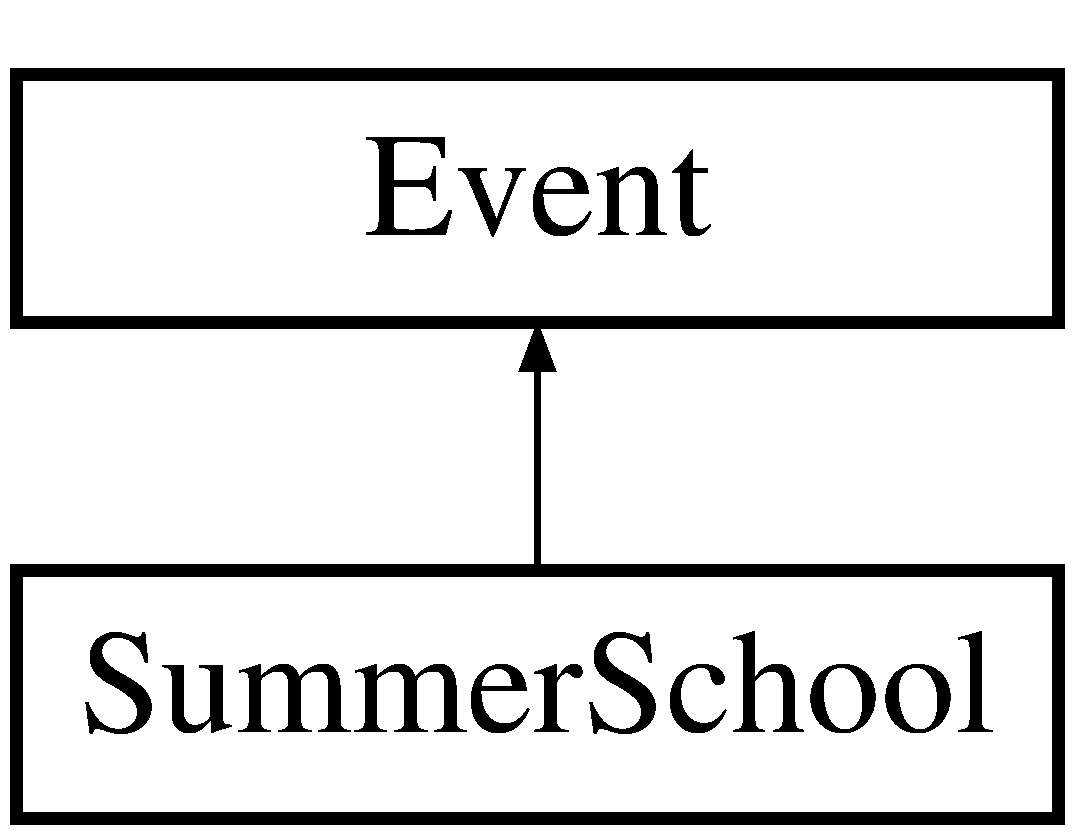
\includegraphics[height=2.000000cm]{classSummerSchool}
\end{center}
\end{figure}
\subsection*{Public Member Functions}
\begin{DoxyCompactItemize}
\item 
\mbox{\hyperlink{classSummerSchool_af66df445834a36ccb6e67d5503c1b776}{Summer\+School}} ()
\item 
\mbox{\hyperlink{classSummerSchool_a108aeb7981fbb9e6dbe44c1425517ddf}{Summer\+School}} (std\+::vector$<$ \mbox{\hyperlink{classAssociate}{Associate}} $\ast$$>$ \mbox{\hyperlink{classEvent_a6cec387dca85f0a0e8419cfc94eb320e}{event\+\_\+request}}, std\+::vector$<$ \mbox{\hyperlink{classAssociate}{Associate}} $\ast$$>$ \mbox{\hyperlink{classEvent_ad35e04c759fdbfad75aed0b6e2eef63c}{event\+\_\+organizers}}, std\+::string \mbox{\hyperlink{classEvent_a9a93c9d38211f84cd6e347690e177f11}{date}}, std\+::string \mbox{\hyperlink{classEvent_a3d1f28a3bde9ab718d5b0003f8ab5129}{local}}, std\+::string \mbox{\hyperlink{classEvent_aa9cc4378d5cecaadc8e6de92b313e6f8}{theme}}, int \mbox{\hyperlink{classEvent_a4059db56458a92ddb5bd1d1443631b02}{phase}}, \mbox{\hyperlink{classAssociation}{Association}} $\ast$\mbox{\hyperlink{classEvent_a3c8694833e50dbd2e37943eff1f5c9b1}{association}}, std\+::list$<$ \mbox{\hyperlink{classTrainer}{Trainer}} $\ast$$>$ \mbox{\hyperlink{classSummerSchool_a3208a977c13ce8d7415b179a040efae3}{trainers}})
\begin{DoxyCompactList}\small\item\em Full \mbox{\hyperlink{classSummerSchool}{Summer\+School}} Constructor. \end{DoxyCompactList}\item 
\mbox{\hyperlink{classSummerSchool_aa9cbb04b10fee38c90a5a02372878383}{Summer\+School}} (std\+::vector$<$ \mbox{\hyperlink{classAssociate}{Associate}} $\ast$$>$ \mbox{\hyperlink{classEvent_a6cec387dca85f0a0e8419cfc94eb320e}{event\+\_\+request}}, std\+::vector$<$ \mbox{\hyperlink{classAssociate}{Associate}} $\ast$$>$ \mbox{\hyperlink{classEvent_ad35e04c759fdbfad75aed0b6e2eef63c}{event\+\_\+organizers}}, std\+::string \mbox{\hyperlink{classEvent_a9a93c9d38211f84cd6e347690e177f11}{date}}, std\+::string \mbox{\hyperlink{classEvent_a3d1f28a3bde9ab718d5b0003f8ab5129}{local}}, std\+::string \mbox{\hyperlink{classEvent_aa9cc4378d5cecaadc8e6de92b313e6f8}{theme}}, int \mbox{\hyperlink{classEvent_a4059db56458a92ddb5bd1d1443631b02}{phase}}, \mbox{\hyperlink{classAssociation}{Association}} $\ast$\mbox{\hyperlink{classEvent_a3c8694833e50dbd2e37943eff1f5c9b1}{association}}, std\+::list$<$ \mbox{\hyperlink{classTrainer}{Trainer}} $\ast$$>$ \mbox{\hyperlink{classSummerSchool_a3208a977c13ce8d7415b179a040efae3}{trainers}}, long double \mbox{\hyperlink{classSummerSchool_a7e6899945d6a486e9d1d1f581236630b}{given\+\_\+support}})
\begin{DoxyCompactList}\small\item\em Full \mbox{\hyperlink{classSummerSchool}{Summer\+School}} Constructor. \end{DoxyCompactList}\item 
virtual \mbox{\hyperlink{classSummerSchool_ad3c3df760cfaee1042fe5290fa487b2c}{$\sim$\+Summer\+School}} ()
\begin{DoxyCompactList}\small\item\em Default \mbox{\hyperlink{classSummerSchool}{Summer\+School}} Destructor. \end{DoxyCompactList}\item 
long double \mbox{\hyperlink{classSummerSchool_a86f34a2f39dcd33171e77c386165219c}{get\+Support}} () const
\begin{DoxyCompactList}\small\item\em Returns the money the \mbox{\hyperlink{classAssociation}{Association}} gave to support the event. \end{DoxyCompactList}\item 
std\+::string \mbox{\hyperlink{classSummerSchool_a2ba547411ca8f161c2c579f9f55f913e}{get\+Type}} () const
\begin{DoxyCompactList}\small\item\em Returns the type of the event. \end{DoxyCompactList}\item 
std\+::list$<$ \mbox{\hyperlink{classTrainer}{Trainer}} $\ast$ $>$ \mbox{\hyperlink{classSummerSchool_aba18410ee9fbafd26858232104b5b39f}{get\+Trainers}} () const
\begin{DoxyCompactList}\small\item\em Returns all the trainers who will lecture during the summer\+School. \end{DoxyCompactList}\item 
int \mbox{\hyperlink{classSummerSchool_a019b9e38108b7dd31cd93cab285d0d00}{get\+Estimative}} () const
\begin{DoxyCompactList}\small\item\em Returns the estimative of people attending the summer\+School. \end{DoxyCompactList}\item 
std\+::string \mbox{\hyperlink{classSummerSchool_a61ac7307840f787e3de639d431248e26}{show\+Info}} () const
\begin{DoxyCompactList}\small\item\em Returns (in a string) all the information about a summer\+School. \end{DoxyCompactList}\end{DoxyCompactItemize}
\subsection*{Private Attributes}
\begin{DoxyCompactItemize}
\item 
std\+::string \mbox{\hyperlink{classSummerSchool_a4bce94c462b492844cacce921427d212}{type}} = \char`\"{}Summer\+School\char`\"{}
\begin{DoxyCompactList}\small\item\em The type of the \mbox{\hyperlink{classEvent}{Event}} (\mbox{\hyperlink{classSummerSchool}{Summer\+School}}) \end{DoxyCompactList}\item 
std\+::list$<$ \mbox{\hyperlink{classTrainer}{Trainer}} $\ast$ $>$ \mbox{\hyperlink{classSummerSchool_a3208a977c13ce8d7415b179a040efae3}{trainers}}
\begin{DoxyCompactList}\small\item\em All trainers in the \mbox{\hyperlink{classSummerSchool}{Summer\+School}}. \end{DoxyCompactList}\item 
long double \mbox{\hyperlink{classSummerSchool_a7e6899945d6a486e9d1d1f581236630b}{given\+\_\+support}}
\begin{DoxyCompactList}\small\item\em The value of the monetary support given by the association. \end{DoxyCompactList}\end{DoxyCompactItemize}
\subsection*{Additional Inherited Members}


\subsection{Detailed Description}
The \mbox{\hyperlink{classSummerSchool}{Summer\+School}} Class -\/ Derived Class from the Super \mbox{\hyperlink{classEvent}{Event}} Class. 

A summer\+School is a special type of event. This one has some trainers who will give lectures during the event 

\subsection{Constructor \& Destructor Documentation}
\mbox{\Hypertarget{classSummerSchool_af66df445834a36ccb6e67d5503c1b776}\label{classSummerSchool_af66df445834a36ccb6e67d5503c1b776}} 
\index{Summer\+School@{Summer\+School}!Summer\+School@{Summer\+School}}
\index{Summer\+School@{Summer\+School}!Summer\+School@{Summer\+School}}
\subsubsection{\texorpdfstring{Summer\+School()}{SummerSchool()}\hspace{0.1cm}{\footnotesize\ttfamily [1/3]}}
{\footnotesize\ttfamily Summer\+School\+::\+Summer\+School (\begin{DoxyParamCaption}{ }\end{DoxyParamCaption})}

\mbox{\Hypertarget{classSummerSchool_a108aeb7981fbb9e6dbe44c1425517ddf}\label{classSummerSchool_a108aeb7981fbb9e6dbe44c1425517ddf}} 
\index{Summer\+School@{Summer\+School}!Summer\+School@{Summer\+School}}
\index{Summer\+School@{Summer\+School}!Summer\+School@{Summer\+School}}
\subsubsection{\texorpdfstring{Summer\+School()}{SummerSchool()}\hspace{0.1cm}{\footnotesize\ttfamily [2/3]}}
{\footnotesize\ttfamily Summer\+School\+::\+Summer\+School (\begin{DoxyParamCaption}\item[{std\+::vector$<$ \mbox{\hyperlink{classAssociate}{Associate}} $\ast$$>$}]{event\+\_\+request,  }\item[{std\+::vector$<$ \mbox{\hyperlink{classAssociate}{Associate}} $\ast$$>$}]{event\+\_\+organizers,  }\item[{std\+::string}]{date,  }\item[{std\+::string}]{local,  }\item[{std\+::string}]{theme,  }\item[{int}]{phase,  }\item[{\mbox{\hyperlink{classAssociation}{Association}} $\ast$}]{association,  }\item[{std\+::list$<$ \mbox{\hyperlink{classTrainer}{Trainer}} $\ast$$>$}]{trainers }\end{DoxyParamCaption})}



Full \mbox{\hyperlink{classSummerSchool}{Summer\+School}} Constructor. 


\begin{DoxyParams}{Parameters}
{\em event\+\_\+request} & -\/ The associates that requested the summerschool (up to 3) \\
\hline
{\em event\+\_\+organizers} & -\/ The associates that requested the summerschool (up to 3) and the ones who will help organize \\
\hline
{\em date} & -\/ The date of the summerschool \\
\hline
{\em local} & -\/ The local of the summerschool \\
\hline
{\em theme} & -\/ The theme of the summerschool \\
\hline
{\em phase} & -\/ The phase of the summerschool \\
\hline
{\em association} & -\/ The \mbox{\hyperlink{classAssociation}{Association}} that promotes the summerschool \\
\hline
{\em trainers} & -\/ A list of all the trainers that will lecture during the summerschool \\
\hline
\end{DoxyParams}
\mbox{\Hypertarget{classSummerSchool_aa9cbb04b10fee38c90a5a02372878383}\label{classSummerSchool_aa9cbb04b10fee38c90a5a02372878383}} 
\index{Summer\+School@{Summer\+School}!Summer\+School@{Summer\+School}}
\index{Summer\+School@{Summer\+School}!Summer\+School@{Summer\+School}}
\subsubsection{\texorpdfstring{Summer\+School()}{SummerSchool()}\hspace{0.1cm}{\footnotesize\ttfamily [3/3]}}
{\footnotesize\ttfamily Summer\+School\+::\+Summer\+School (\begin{DoxyParamCaption}\item[{std\+::vector$<$ \mbox{\hyperlink{classAssociate}{Associate}} $\ast$$>$}]{event\+\_\+request,  }\item[{std\+::vector$<$ \mbox{\hyperlink{classAssociate}{Associate}} $\ast$$>$}]{event\+\_\+organizers,  }\item[{std\+::string}]{date,  }\item[{std\+::string}]{local,  }\item[{std\+::string}]{theme,  }\item[{int}]{phase,  }\item[{\mbox{\hyperlink{classAssociation}{Association}} $\ast$}]{association,  }\item[{std\+::list$<$ \mbox{\hyperlink{classTrainer}{Trainer}} $\ast$$>$}]{trainers,  }\item[{long double}]{given\+\_\+support }\end{DoxyParamCaption})}



Full \mbox{\hyperlink{classSummerSchool}{Summer\+School}} Constructor. 


\begin{DoxyParams}{Parameters}
{\em event\+\_\+request} & -\/ The associates that requested the summerschool (up to 3) \\
\hline
{\em event\+\_\+organizers} & -\/ The associates that requested the summerschool (up to 3) and the ones who will help organize \\
\hline
{\em date} & -\/ The date of the summerschool \\
\hline
{\em local} & -\/ The local of the summerschool \\
\hline
{\em theme} & -\/ The theme of the summerschool \\
\hline
{\em phase} & -\/ The phase of the summerschool \\
\hline
{\em association} & -\/ The \mbox{\hyperlink{classAssociation}{Association}} that promotes the summerschool \\
\hline
{\em trainers} & -\/ A list of all the trainers that will lecture during the summerschool \\
\hline
{\em give\+\_\+support} & -\/ The amount the \mbox{\hyperlink{classAssociation}{Association}} gives to promote de event \\
\hline
\end{DoxyParams}
\mbox{\Hypertarget{classSummerSchool_ad3c3df760cfaee1042fe5290fa487b2c}\label{classSummerSchool_ad3c3df760cfaee1042fe5290fa487b2c}} 
\index{Summer\+School@{Summer\+School}!````~Summer\+School@{$\sim$\+Summer\+School}}
\index{````~Summer\+School@{$\sim$\+Summer\+School}!Summer\+School@{Summer\+School}}
\subsubsection{\texorpdfstring{$\sim$\+Summer\+School()}{~SummerSchool()}}
{\footnotesize\ttfamily Summer\+School\+::$\sim$\+Summer\+School (\begin{DoxyParamCaption}{ }\end{DoxyParamCaption})\hspace{0.3cm}{\ttfamily [virtual]}}



Default \mbox{\hyperlink{classSummerSchool}{Summer\+School}} Destructor. 



\subsection{Member Function Documentation}
\mbox{\Hypertarget{classSummerSchool_a019b9e38108b7dd31cd93cab285d0d00}\label{classSummerSchool_a019b9e38108b7dd31cd93cab285d0d00}} 
\index{Summer\+School@{Summer\+School}!get\+Estimative@{get\+Estimative}}
\index{get\+Estimative@{get\+Estimative}!Summer\+School@{Summer\+School}}
\subsubsection{\texorpdfstring{get\+Estimative()}{getEstimative()}}
{\footnotesize\ttfamily int Summer\+School\+::get\+Estimative (\begin{DoxyParamCaption}{ }\end{DoxyParamCaption}) const\hspace{0.3cm}{\ttfamily [virtual]}}



Returns the estimative of people attending the summer\+School. 



Implements \mbox{\hyperlink{classEvent_a18ac55c239f648fc0ad5687c426f2a8f}{Event}}.

\mbox{\Hypertarget{classSummerSchool_a86f34a2f39dcd33171e77c386165219c}\label{classSummerSchool_a86f34a2f39dcd33171e77c386165219c}} 
\index{Summer\+School@{Summer\+School}!get\+Support@{get\+Support}}
\index{get\+Support@{get\+Support}!Summer\+School@{Summer\+School}}
\subsubsection{\texorpdfstring{get\+Support()}{getSupport()}}
{\footnotesize\ttfamily long double Summer\+School\+::get\+Support (\begin{DoxyParamCaption}{ }\end{DoxyParamCaption}) const\hspace{0.3cm}{\ttfamily [virtual]}}



Returns the money the \mbox{\hyperlink{classAssociation}{Association}} gave to support the event. 



Implements \mbox{\hyperlink{classEvent_a9170bfcbd9b00015dafc5d5cc69a2cfe}{Event}}.

\mbox{\Hypertarget{classSummerSchool_aba18410ee9fbafd26858232104b5b39f}\label{classSummerSchool_aba18410ee9fbafd26858232104b5b39f}} 
\index{Summer\+School@{Summer\+School}!get\+Trainers@{get\+Trainers}}
\index{get\+Trainers@{get\+Trainers}!Summer\+School@{Summer\+School}}
\subsubsection{\texorpdfstring{get\+Trainers()}{getTrainers()}}
{\footnotesize\ttfamily list$<$ \mbox{\hyperlink{classTrainer}{Trainer}} $\ast$ $>$ Summer\+School\+::get\+Trainers (\begin{DoxyParamCaption}{ }\end{DoxyParamCaption}) const\hspace{0.3cm}{\ttfamily [virtual]}}



Returns all the trainers who will lecture during the summer\+School. 



Implements \mbox{\hyperlink{classEvent_a11aad3e5a7ee85bc61b6811d050c5d70}{Event}}.

\mbox{\Hypertarget{classSummerSchool_a2ba547411ca8f161c2c579f9f55f913e}\label{classSummerSchool_a2ba547411ca8f161c2c579f9f55f913e}} 
\index{Summer\+School@{Summer\+School}!get\+Type@{get\+Type}}
\index{get\+Type@{get\+Type}!Summer\+School@{Summer\+School}}
\subsubsection{\texorpdfstring{get\+Type()}{getType()}}
{\footnotesize\ttfamily string Summer\+School\+::get\+Type (\begin{DoxyParamCaption}{ }\end{DoxyParamCaption}) const\hspace{0.3cm}{\ttfamily [virtual]}}



Returns the type of the event. 



Implements \mbox{\hyperlink{classEvent_a224dbd9a9aee5937ba0c8ea1a056af1f}{Event}}.

\mbox{\Hypertarget{classSummerSchool_a61ac7307840f787e3de639d431248e26}\label{classSummerSchool_a61ac7307840f787e3de639d431248e26}} 
\index{Summer\+School@{Summer\+School}!show\+Info@{show\+Info}}
\index{show\+Info@{show\+Info}!Summer\+School@{Summer\+School}}
\subsubsection{\texorpdfstring{show\+Info()}{showInfo()}}
{\footnotesize\ttfamily string Summer\+School\+::show\+Info (\begin{DoxyParamCaption}{ }\end{DoxyParamCaption}) const\hspace{0.3cm}{\ttfamily [virtual]}}



Returns (in a string) all the information about a summer\+School. 



Implements \mbox{\hyperlink{classEvent_aaa38f467e933c57190d43351bdb817be}{Event}}.



\subsection{Member Data Documentation}
\mbox{\Hypertarget{classSummerSchool_a7e6899945d6a486e9d1d1f581236630b}\label{classSummerSchool_a7e6899945d6a486e9d1d1f581236630b}} 
\index{Summer\+School@{Summer\+School}!given\+\_\+support@{given\+\_\+support}}
\index{given\+\_\+support@{given\+\_\+support}!Summer\+School@{Summer\+School}}
\subsubsection{\texorpdfstring{given\+\_\+support}{given\_support}}
{\footnotesize\ttfamily long double Summer\+School\+::given\+\_\+support\hspace{0.3cm}{\ttfamily [private]}}



The value of the monetary support given by the association. 

\mbox{\Hypertarget{classSummerSchool_a3208a977c13ce8d7415b179a040efae3}\label{classSummerSchool_a3208a977c13ce8d7415b179a040efae3}} 
\index{Summer\+School@{Summer\+School}!trainers@{trainers}}
\index{trainers@{trainers}!Summer\+School@{Summer\+School}}
\subsubsection{\texorpdfstring{trainers}{trainers}}
{\footnotesize\ttfamily std\+::list$<$\mbox{\hyperlink{classTrainer}{Trainer}} $\ast$$>$ Summer\+School\+::trainers\hspace{0.3cm}{\ttfamily [private]}}



All trainers in the \mbox{\hyperlink{classSummerSchool}{Summer\+School}}. 

\mbox{\Hypertarget{classSummerSchool_a4bce94c462b492844cacce921427d212}\label{classSummerSchool_a4bce94c462b492844cacce921427d212}} 
\index{Summer\+School@{Summer\+School}!type@{type}}
\index{type@{type}!Summer\+School@{Summer\+School}}
\subsubsection{\texorpdfstring{type}{type}}
{\footnotesize\ttfamily std\+::string Summer\+School\+::type = \char`\"{}Summer\+School\char`\"{}\hspace{0.3cm}{\ttfamily [private]}}



The type of the \mbox{\hyperlink{classEvent}{Event}} (\mbox{\hyperlink{classSummerSchool}{Summer\+School}}) 



The documentation for this class was generated from the following files\+:\begin{DoxyCompactItemize}
\item 
\mbox{\hyperlink{SummerSchool_8h}{Summer\+School.\+h}}\item 
\mbox{\hyperlink{SummerSchool_8cpp}{Summer\+School.\+cpp}}\end{DoxyCompactItemize}

\hypertarget{classTrainer}{}\section{Trainer Class Reference}
\label{classTrainer}\index{Trainer@{Trainer}}


The \mbox{\hyperlink{classTrainer}{Trainer}} Class.  




{\ttfamily \#include $<$Summer\+School.\+h$>$}

\subsection*{Public Member Functions}
\begin{DoxyCompactItemize}
\item 
\mbox{\hyperlink{classTrainer_ae033382eaedd47966c8667439376369a}{Trainer}} (std\+::string \mbox{\hyperlink{classTrainer_a6b58d4cfdb8d3482cb2c09dd366a6350}{name}}, std\+::string \mbox{\hyperlink{classTrainer_ae895aa7f146d8bf271399215d4ede36b}{institution}})
\begin{DoxyCompactList}\small\item\em Full \mbox{\hyperlink{classTrainer}{Trainer}} Constructor. \end{DoxyCompactList}\item 
\mbox{\hyperlink{classTrainer_aa3d993d1eb090f4111e12a710fe9d3f6}{$\sim$\+Trainer}} ()
\begin{DoxyCompactList}\small\item\em Default \mbox{\hyperlink{classTrainer}{Trainer}} Destructor. \end{DoxyCompactList}\item 
std\+::string \mbox{\hyperlink{classTrainer_a4bf23e8eaefc7c2f400b4ba14f2e1c69}{get\+Name}} () const
\begin{DoxyCompactList}\small\item\em Returns the name of the trainer. \end{DoxyCompactList}\item 
std\+::string \mbox{\hyperlink{classTrainer_a92ce4244bea56ae32c0ba33fdd959667}{get\+Institution}} () const
\begin{DoxyCompactList}\small\item\em Returns the institution of the trainer. \end{DoxyCompactList}\end{DoxyCompactItemize}
\subsection*{Private Attributes}
\begin{DoxyCompactItemize}
\item 
std\+::string \mbox{\hyperlink{classTrainer_a6b58d4cfdb8d3482cb2c09dd366a6350}{name}}
\begin{DoxyCompactList}\small\item\em The name of the trainer. \end{DoxyCompactList}\item 
std\+::string \mbox{\hyperlink{classTrainer_ae895aa7f146d8bf271399215d4ede36b}{institution}}
\begin{DoxyCompactList}\small\item\em The institution of the trainer. \end{DoxyCompactList}\end{DoxyCompactItemize}


\subsection{Detailed Description}
The \mbox{\hyperlink{classTrainer}{Trainer}} Class. 

Trainers are the people who lecture during the summerschools 

\subsection{Constructor \& Destructor Documentation}
\mbox{\Hypertarget{classTrainer_ae033382eaedd47966c8667439376369a}\label{classTrainer_ae033382eaedd47966c8667439376369a}} 
\index{Trainer@{Trainer}!Trainer@{Trainer}}
\index{Trainer@{Trainer}!Trainer@{Trainer}}
\subsubsection{\texorpdfstring{Trainer()}{Trainer()}}
{\footnotesize\ttfamily Trainer\+::\+Trainer (\begin{DoxyParamCaption}\item[{std\+::string}]{name,  }\item[{std\+::string}]{institution }\end{DoxyParamCaption})\hspace{0.3cm}{\ttfamily [inline]}}



Full \mbox{\hyperlink{classTrainer}{Trainer}} Constructor. 


\begin{DoxyParams}{Parameters}
{\em name} & -\/ The name of the trainer \\
\hline
{\em institution} & -\/ The institution of the trainer \\
\hline
\end{DoxyParams}
\mbox{\Hypertarget{classTrainer_aa3d993d1eb090f4111e12a710fe9d3f6}\label{classTrainer_aa3d993d1eb090f4111e12a710fe9d3f6}} 
\index{Trainer@{Trainer}!````~Trainer@{$\sim$\+Trainer}}
\index{````~Trainer@{$\sim$\+Trainer}!Trainer@{Trainer}}
\subsubsection{\texorpdfstring{$\sim$\+Trainer()}{~Trainer()}}
{\footnotesize\ttfamily Trainer\+::$\sim$\+Trainer (\begin{DoxyParamCaption}{ }\end{DoxyParamCaption})}



Default \mbox{\hyperlink{classTrainer}{Trainer}} Destructor. 



\subsection{Member Function Documentation}
\mbox{\Hypertarget{classTrainer_a92ce4244bea56ae32c0ba33fdd959667}\label{classTrainer_a92ce4244bea56ae32c0ba33fdd959667}} 
\index{Trainer@{Trainer}!get\+Institution@{get\+Institution}}
\index{get\+Institution@{get\+Institution}!Trainer@{Trainer}}
\subsubsection{\texorpdfstring{get\+Institution()}{getInstitution()}}
{\footnotesize\ttfamily std\+::string Trainer\+::get\+Institution (\begin{DoxyParamCaption}{ }\end{DoxyParamCaption}) const\hspace{0.3cm}{\ttfamily [inline]}}



Returns the institution of the trainer. 

\mbox{\Hypertarget{classTrainer_a4bf23e8eaefc7c2f400b4ba14f2e1c69}\label{classTrainer_a4bf23e8eaefc7c2f400b4ba14f2e1c69}} 
\index{Trainer@{Trainer}!get\+Name@{get\+Name}}
\index{get\+Name@{get\+Name}!Trainer@{Trainer}}
\subsubsection{\texorpdfstring{get\+Name()}{getName()}}
{\footnotesize\ttfamily std\+::string Trainer\+::get\+Name (\begin{DoxyParamCaption}{ }\end{DoxyParamCaption}) const\hspace{0.3cm}{\ttfamily [inline]}}



Returns the name of the trainer. 



\subsection{Member Data Documentation}
\mbox{\Hypertarget{classTrainer_ae895aa7f146d8bf271399215d4ede36b}\label{classTrainer_ae895aa7f146d8bf271399215d4ede36b}} 
\index{Trainer@{Trainer}!institution@{institution}}
\index{institution@{institution}!Trainer@{Trainer}}
\subsubsection{\texorpdfstring{institution}{institution}}
{\footnotesize\ttfamily std\+::string Trainer\+::institution\hspace{0.3cm}{\ttfamily [private]}}



The institution of the trainer. 

\mbox{\Hypertarget{classTrainer_a6b58d4cfdb8d3482cb2c09dd366a6350}\label{classTrainer_a6b58d4cfdb8d3482cb2c09dd366a6350}} 
\index{Trainer@{Trainer}!name@{name}}
\index{name@{name}!Trainer@{Trainer}}
\subsubsection{\texorpdfstring{name}{name}}
{\footnotesize\ttfamily std\+::string Trainer\+::name\hspace{0.3cm}{\ttfamily [private]}}



The name of the trainer. 



The documentation for this class was generated from the following file\+:\begin{DoxyCompactItemize}
\item 
\mbox{\hyperlink{SummerSchool_8h}{Summer\+School.\+h}}\end{DoxyCompactItemize}

\chapter{File Documentation}
\hypertarget{Area_8cpp}{}\section{Area.\+cpp File Reference}
\label{Area_8cpp}\index{Area.\+cpp@{Area.\+cpp}}
{\ttfamily \#include \char`\"{}Area.\+h\char`\"{}}\newline
{\ttfamily \#include \char`\"{}Sub\+Area.\+h\char`\"{}}\newline
{\ttfamily \#include $<$sstream$>$}\newline
{\ttfamily \#include $<$iostream$>$}\newline

\hypertarget{Area_8h}{}\section{Area.\+h File Reference}
\label{Area_8h}\index{Area.\+h@{Area.\+h}}
{\ttfamily \#include $<$string$>$}\newline
{\ttfamily \#include $<$vector$>$}\newline
\subsection*{Classes}
\begin{DoxyCompactItemize}
\item 
class \mbox{\hyperlink{classArea}{Area}}
\begin{DoxyCompactList}\small\item\em The \mbox{\hyperlink{classArea}{Area}} Class. \end{DoxyCompactList}\end{DoxyCompactItemize}

\hypertarget{Associate_8cpp}{}\section{Associate.\+cpp File Reference}
\label{Associate_8cpp}\index{Associate.\+cpp@{Associate.\+cpp}}
{\ttfamily \#include \char`\"{}Associate.\+h\char`\"{}}\newline
{\ttfamily \#include \char`\"{}Area.\+h\char`\"{}}\newline
{\ttfamily \#include \char`\"{}Sub\+Area.\+h\char`\"{}}\newline
{\ttfamily \#include \char`\"{}Association.\+h\char`\"{}}\newline
{\ttfamily \#include $<$sstream$>$}\newline
{\ttfamily \#include $<$iostream$>$}\newline
{\ttfamily \#include $<$iomanip$>$}\newline

\hypertarget{Associate_8h}{}\section{Associate.\+h File Reference}
\label{Associate_8h}\index{Associate.\+h@{Associate.\+h}}
{\ttfamily \#include $<$vector$>$}\newline
{\ttfamily \#include $<$string$>$}\newline
\subsection*{Classes}
\begin{DoxyCompactItemize}
\item 
class \hyperlink{classNotUpToDate}{Not\+Up\+To\+Date}
\begin{DoxyCompactList}\small\item\em The \hyperlink{classNotUpToDate}{Not\+Up\+To\+Date} Class. \end{DoxyCompactList}\item 
class \hyperlink{classNotEnoughMoney}{Not\+Enough\+Money}
\begin{DoxyCompactList}\small\item\em The \hyperlink{classNotEnoughMoney}{Not\+Enough\+Money} Class. \end{DoxyCompactList}\item 
class \hyperlink{classAlreadyPaid}{Already\+Paid}
\begin{DoxyCompactList}\small\item\em The Not\+Already\+Paid Class. \end{DoxyCompactList}\item 
class \hyperlink{classAssociate}{Associate}
\begin{DoxyCompactList}\small\item\em The \hyperlink{classAssociate}{Associate} Class. \end{DoxyCompactList}\end{DoxyCompactItemize}

\hypertarget{Association_8cpp}{}\section{Association.\+cpp File Reference}
\label{Association_8cpp}\index{Association.\+cpp@{Association.\+cpp}}
{\ttfamily \#include \char`\"{}Association.\+h\char`\"{}}\newline
{\ttfamily \#include \char`\"{}Associate.\+h\char`\"{}}\newline
{\ttfamily \#include \char`\"{}Area.\+h\char`\"{}}\newline
{\ttfamily \#include \char`\"{}Sub\+Area.\+h\char`\"{}}\newline
{\ttfamily \#include \char`\"{}Event.\+h\char`\"{}}\newline
{\ttfamily \#include $<$algorithm$>$}\newline
{\ttfamily \#include $<$sstream$>$}\newline
{\ttfamily \#include $<$iostream$>$}\newline
\subsection*{Functions}
\begin{DoxyCompactItemize}
\item 
bool \hyperlink{Association_8cpp_a7212dfc6bb07893e23fa977f18309ded}{cmp\+ID} (\hyperlink{classAssociate}{Associate} $\ast$rhs, \hyperlink{classAssociate}{Associate} $\ast$lhs)
\begin{DoxyCompactList}\small\item\em compares the ID of 2 different associates \end{DoxyCompactList}\item 
bool \hyperlink{Association_8cpp_acd1fd4877ff6b5bf584be877a13d0588}{cmp\+Money} (\hyperlink{classAssociate}{Associate} $\ast$rhs, \hyperlink{classAssociate}{Associate} $\ast$lhs)
\begin{DoxyCompactList}\small\item\em compares the money of 2 different associates \end{DoxyCompactList}\item 
{\footnotesize template$<$class T $>$ }\\bool \hyperlink{Association_8cpp_a49e957f0e7f022406e6c81895eed79b7}{cmp\+Name} (T $\ast$rhs, T $\ast$lhs)
\begin{DoxyCompactList}\small\item\em compares the name of 2 different associates \end{DoxyCompactList}\item 
bool \hyperlink{Association_8cpp_a0d94d17cdf7ce760c4d131d58d6eb48a}{cmp\+Date} (\hyperlink{classEvent}{Event} $\ast$rhs, \hyperlink{classEvent}{Event} $\ast$lhs)
\begin{DoxyCompactList}\small\item\em compares 2 dates \end{DoxyCompactList}\item 
bool \hyperlink{Association_8cpp_aec8efa10619563981c3aaf91e3889b18}{cmp\+Local} (\hyperlink{classEvent}{Event} $\ast$rhs, \hyperlink{classEvent}{Event} $\ast$lhs)
\begin{DoxyCompactList}\small\item\em compares 2 locals \end{DoxyCompactList}\item 
bool \hyperlink{Association_8cpp_a02d68dc36b7585e8b71298fa2f21d610}{cmp\+Theme} (\hyperlink{classEvent}{Event} $\ast$rhs, \hyperlink{classEvent}{Event} $\ast$lhs)
\begin{DoxyCompactList}\small\item\em compares 2 themes \end{DoxyCompactList}\end{DoxyCompactItemize}


\subsection{Function Documentation}
\mbox{\Hypertarget{Association_8cpp_a0d94d17cdf7ce760c4d131d58d6eb48a}\label{Association_8cpp_a0d94d17cdf7ce760c4d131d58d6eb48a}} 
\index{Association.\+cpp@{Association.\+cpp}!cmp\+Date@{cmp\+Date}}
\index{cmp\+Date@{cmp\+Date}!Association.\+cpp@{Association.\+cpp}}
\subsubsection{\texorpdfstring{cmp\+Date()}{cmpDate()}}
{\footnotesize\ttfamily bool cmp\+Date (\begin{DoxyParamCaption}\item[{\hyperlink{classEvent}{Event} $\ast$}]{rhs,  }\item[{\hyperlink{classEvent}{Event} $\ast$}]{lhs }\end{DoxyParamCaption})}



compares 2 dates 


\begin{DoxyParams}{Parameters}
{\em rhs} & -\/ First date \\
\hline
{\em lhs} & -\/ Second date \\
\hline
\end{DoxyParams}
\mbox{\Hypertarget{Association_8cpp_a7212dfc6bb07893e23fa977f18309ded}\label{Association_8cpp_a7212dfc6bb07893e23fa977f18309ded}} 
\index{Association.\+cpp@{Association.\+cpp}!cmp\+ID@{cmp\+ID}}
\index{cmp\+ID@{cmp\+ID}!Association.\+cpp@{Association.\+cpp}}
\subsubsection{\texorpdfstring{cmp\+I\+D()}{cmpID()}}
{\footnotesize\ttfamily bool cmp\+ID (\begin{DoxyParamCaption}\item[{\hyperlink{classAssociate}{Associate} $\ast$}]{rhs,  }\item[{\hyperlink{classAssociate}{Associate} $\ast$}]{lhs }\end{DoxyParamCaption})}



compares the ID of 2 different associates 


\begin{DoxyParams}{Parameters}
{\em rhs} & -\/ First associate \\
\hline
{\em lhs} & -\/ Second associate \\
\hline
\end{DoxyParams}
\mbox{\Hypertarget{Association_8cpp_aec8efa10619563981c3aaf91e3889b18}\label{Association_8cpp_aec8efa10619563981c3aaf91e3889b18}} 
\index{Association.\+cpp@{Association.\+cpp}!cmp\+Local@{cmp\+Local}}
\index{cmp\+Local@{cmp\+Local}!Association.\+cpp@{Association.\+cpp}}
\subsubsection{\texorpdfstring{cmp\+Local()}{cmpLocal()}}
{\footnotesize\ttfamily bool cmp\+Local (\begin{DoxyParamCaption}\item[{\hyperlink{classEvent}{Event} $\ast$}]{rhs,  }\item[{\hyperlink{classEvent}{Event} $\ast$}]{lhs }\end{DoxyParamCaption})}



compares 2 locals 


\begin{DoxyParams}{Parameters}
{\em rhs} & -\/ First local \\
\hline
{\em lhs} & -\/ Second local \\
\hline
\end{DoxyParams}
\mbox{\Hypertarget{Association_8cpp_acd1fd4877ff6b5bf584be877a13d0588}\label{Association_8cpp_acd1fd4877ff6b5bf584be877a13d0588}} 
\index{Association.\+cpp@{Association.\+cpp}!cmp\+Money@{cmp\+Money}}
\index{cmp\+Money@{cmp\+Money}!Association.\+cpp@{Association.\+cpp}}
\subsubsection{\texorpdfstring{cmp\+Money()}{cmpMoney()}}
{\footnotesize\ttfamily bool cmp\+Money (\begin{DoxyParamCaption}\item[{\hyperlink{classAssociate}{Associate} $\ast$}]{rhs,  }\item[{\hyperlink{classAssociate}{Associate} $\ast$}]{lhs }\end{DoxyParamCaption})}



compares the money of 2 different associates 


\begin{DoxyParams}{Parameters}
{\em rhs} & -\/ First associate \\
\hline
{\em lhs} & -\/ Second associate \\
\hline
\end{DoxyParams}
\mbox{\Hypertarget{Association_8cpp_a49e957f0e7f022406e6c81895eed79b7}\label{Association_8cpp_a49e957f0e7f022406e6c81895eed79b7}} 
\index{Association.\+cpp@{Association.\+cpp}!cmp\+Name@{cmp\+Name}}
\index{cmp\+Name@{cmp\+Name}!Association.\+cpp@{Association.\+cpp}}
\subsubsection{\texorpdfstring{cmp\+Name()}{cmpName()}}
{\footnotesize\ttfamily template$<$class T $>$ \\
bool cmp\+Name (\begin{DoxyParamCaption}\item[{T $\ast$}]{rhs,  }\item[{T $\ast$}]{lhs }\end{DoxyParamCaption})}



compares the name of 2 different associates 


\begin{DoxyParams}{Parameters}
{\em rhs} & -\/ First associate \\
\hline
{\em lhs} & -\/ Second associate \\
\hline
\end{DoxyParams}
\mbox{\Hypertarget{Association_8cpp_a02d68dc36b7585e8b71298fa2f21d610}\label{Association_8cpp_a02d68dc36b7585e8b71298fa2f21d610}} 
\index{Association.\+cpp@{Association.\+cpp}!cmp\+Theme@{cmp\+Theme}}
\index{cmp\+Theme@{cmp\+Theme}!Association.\+cpp@{Association.\+cpp}}
\subsubsection{\texorpdfstring{cmp\+Theme()}{cmpTheme()}}
{\footnotesize\ttfamily bool cmp\+Theme (\begin{DoxyParamCaption}\item[{\hyperlink{classEvent}{Event} $\ast$}]{rhs,  }\item[{\hyperlink{classEvent}{Event} $\ast$}]{lhs }\end{DoxyParamCaption})}



compares 2 themes 


\begin{DoxyParams}{Parameters}
{\em rhs} & -\/ First theme \\
\hline
{\em lhs} & -\/ Second theme \\
\hline
\end{DoxyParams}

\hypertarget{Association_8h}{}\section{Association.\+h File Reference}
\label{Association_8h}\index{Association.\+h@{Association.\+h}}
{\ttfamily \#include $<$vector$>$}\newline
{\ttfamily \#include $<$string$>$}\newline
{\ttfamily \#include $<$algorithm$>$}\newline
\subsection*{Classes}
\begin{DoxyCompactItemize}
\item 
class \hyperlink{classNoSuchID}{No\+Such\+ID}
\begin{DoxyCompactList}\small\item\em The \hyperlink{classNoSuchID}{No\+Such\+ID} Class. \end{DoxyCompactList}\item 
class \hyperlink{classNoSuchDate}{No\+Such\+Date}
\begin{DoxyCompactList}\small\item\em The \hyperlink{classNoSuchDate}{No\+Such\+Date} Class. \end{DoxyCompactList}\item 
class \hyperlink{classAssociation}{Association}
\begin{DoxyCompactList}\small\item\em The \hyperlink{classAssociation}{Association} Class. \end{DoxyCompactList}\end{DoxyCompactItemize}
\subsection*{Functions}
\begin{DoxyCompactItemize}
\item 
bool \hyperlink{Association_8h_a7212dfc6bb07893e23fa977f18309ded}{cmp\+ID} (\hyperlink{classAssociate}{Associate} $\ast$rhs, \hyperlink{classAssociate}{Associate} $\ast$lhs)
\begin{DoxyCompactList}\small\item\em compares the ID of 2 different associates \end{DoxyCompactList}\item 
bool \hyperlink{Association_8h_acd1fd4877ff6b5bf584be877a13d0588}{cmp\+Money} (\hyperlink{classAssociate}{Associate} $\ast$rhs, \hyperlink{classAssociate}{Associate} $\ast$lhs)
\begin{DoxyCompactList}\small\item\em compares the money of 2 different associates \end{DoxyCompactList}\item 
{\footnotesize template$<$class T $>$ }\\bool \hyperlink{Association_8h_a49e957f0e7f022406e6c81895eed79b7}{cmp\+Name} (T $\ast$rhs, T $\ast$lhs)
\begin{DoxyCompactList}\small\item\em compares the name of 2 different associates \end{DoxyCompactList}\item 
bool \hyperlink{Association_8h_a0d94d17cdf7ce760c4d131d58d6eb48a}{cmp\+Date} (\hyperlink{classEvent}{Event} $\ast$rhs, \hyperlink{classEvent}{Event} $\ast$lhs)
\begin{DoxyCompactList}\small\item\em compares 2 dates \end{DoxyCompactList}\item 
bool \hyperlink{Association_8h_aec8efa10619563981c3aaf91e3889b18}{cmp\+Local} (\hyperlink{classEvent}{Event} $\ast$rhs, \hyperlink{classEvent}{Event} $\ast$lhs)
\begin{DoxyCompactList}\small\item\em compares 2 locals \end{DoxyCompactList}\item 
bool \hyperlink{Association_8h_a02d68dc36b7585e8b71298fa2f21d610}{cmp\+Theme} (\hyperlink{classEvent}{Event} $\ast$rhs, \hyperlink{classEvent}{Event} $\ast$lhs)
\begin{DoxyCompactList}\small\item\em compares 2 themes \end{DoxyCompactList}\end{DoxyCompactItemize}


\subsection{Function Documentation}
\mbox{\Hypertarget{Association_8h_a0d94d17cdf7ce760c4d131d58d6eb48a}\label{Association_8h_a0d94d17cdf7ce760c4d131d58d6eb48a}} 
\index{Association.\+h@{Association.\+h}!cmp\+Date@{cmp\+Date}}
\index{cmp\+Date@{cmp\+Date}!Association.\+h@{Association.\+h}}
\subsubsection{\texorpdfstring{cmp\+Date()}{cmpDate()}}
{\footnotesize\ttfamily bool cmp\+Date (\begin{DoxyParamCaption}\item[{\hyperlink{classEvent}{Event} $\ast$}]{rhs,  }\item[{\hyperlink{classEvent}{Event} $\ast$}]{lhs }\end{DoxyParamCaption})}



compares 2 dates 


\begin{DoxyParams}{Parameters}
{\em rhs} & -\/ First date \\
\hline
{\em lhs} & -\/ Second date \\
\hline
\end{DoxyParams}
\mbox{\Hypertarget{Association_8h_a7212dfc6bb07893e23fa977f18309ded}\label{Association_8h_a7212dfc6bb07893e23fa977f18309ded}} 
\index{Association.\+h@{Association.\+h}!cmp\+ID@{cmp\+ID}}
\index{cmp\+ID@{cmp\+ID}!Association.\+h@{Association.\+h}}
\subsubsection{\texorpdfstring{cmp\+I\+D()}{cmpID()}}
{\footnotesize\ttfamily bool cmp\+ID (\begin{DoxyParamCaption}\item[{\hyperlink{classAssociate}{Associate} $\ast$}]{rhs,  }\item[{\hyperlink{classAssociate}{Associate} $\ast$}]{lhs }\end{DoxyParamCaption})}



compares the ID of 2 different associates 


\begin{DoxyParams}{Parameters}
{\em rhs} & -\/ First associate \\
\hline
{\em lhs} & -\/ Second associate \\
\hline
\end{DoxyParams}
\mbox{\Hypertarget{Association_8h_aec8efa10619563981c3aaf91e3889b18}\label{Association_8h_aec8efa10619563981c3aaf91e3889b18}} 
\index{Association.\+h@{Association.\+h}!cmp\+Local@{cmp\+Local}}
\index{cmp\+Local@{cmp\+Local}!Association.\+h@{Association.\+h}}
\subsubsection{\texorpdfstring{cmp\+Local()}{cmpLocal()}}
{\footnotesize\ttfamily bool cmp\+Local (\begin{DoxyParamCaption}\item[{\hyperlink{classEvent}{Event} $\ast$}]{rhs,  }\item[{\hyperlink{classEvent}{Event} $\ast$}]{lhs }\end{DoxyParamCaption})}



compares 2 locals 


\begin{DoxyParams}{Parameters}
{\em rhs} & -\/ First local \\
\hline
{\em lhs} & -\/ Second local \\
\hline
\end{DoxyParams}
\mbox{\Hypertarget{Association_8h_acd1fd4877ff6b5bf584be877a13d0588}\label{Association_8h_acd1fd4877ff6b5bf584be877a13d0588}} 
\index{Association.\+h@{Association.\+h}!cmp\+Money@{cmp\+Money}}
\index{cmp\+Money@{cmp\+Money}!Association.\+h@{Association.\+h}}
\subsubsection{\texorpdfstring{cmp\+Money()}{cmpMoney()}}
{\footnotesize\ttfamily bool cmp\+Money (\begin{DoxyParamCaption}\item[{\hyperlink{classAssociate}{Associate} $\ast$}]{rhs,  }\item[{\hyperlink{classAssociate}{Associate} $\ast$}]{lhs }\end{DoxyParamCaption})}



compares the money of 2 different associates 


\begin{DoxyParams}{Parameters}
{\em rhs} & -\/ First associate \\
\hline
{\em lhs} & -\/ Second associate \\
\hline
\end{DoxyParams}
\mbox{\Hypertarget{Association_8h_a49e957f0e7f022406e6c81895eed79b7}\label{Association_8h_a49e957f0e7f022406e6c81895eed79b7}} 
\index{Association.\+h@{Association.\+h}!cmp\+Name@{cmp\+Name}}
\index{cmp\+Name@{cmp\+Name}!Association.\+h@{Association.\+h}}
\subsubsection{\texorpdfstring{cmp\+Name()}{cmpName()}}
{\footnotesize\ttfamily template$<$class T $>$ \\
bool cmp\+Name (\begin{DoxyParamCaption}\item[{T $\ast$}]{rhs,  }\item[{T $\ast$}]{lhs }\end{DoxyParamCaption})}



compares the name of 2 different associates 


\begin{DoxyParams}{Parameters}
{\em rhs} & -\/ First associate \\
\hline
{\em lhs} & -\/ Second associate \\
\hline
\end{DoxyParams}
\mbox{\Hypertarget{Association_8h_a02d68dc36b7585e8b71298fa2f21d610}\label{Association_8h_a02d68dc36b7585e8b71298fa2f21d610}} 
\index{Association.\+h@{Association.\+h}!cmp\+Theme@{cmp\+Theme}}
\index{cmp\+Theme@{cmp\+Theme}!Association.\+h@{Association.\+h}}
\subsubsection{\texorpdfstring{cmp\+Theme()}{cmpTheme()}}
{\footnotesize\ttfamily bool cmp\+Theme (\begin{DoxyParamCaption}\item[{\hyperlink{classEvent}{Event} $\ast$}]{rhs,  }\item[{\hyperlink{classEvent}{Event} $\ast$}]{lhs }\end{DoxyParamCaption})}



compares 2 themes 


\begin{DoxyParams}{Parameters}
{\em rhs} & -\/ First theme \\
\hline
{\em lhs} & -\/ Second theme \\
\hline
\end{DoxyParams}

\hypertarget{Conference_8cpp}{}\section{Conference.\+cpp File Reference}
\label{Conference_8cpp}\index{Conference.\+cpp@{Conference.\+cpp}}
{\ttfamily \#include \char`\"{}Conference.\+h\char`\"{}}\newline
{\ttfamily \#include \char`\"{}Association.\+h\char`\"{}}\newline
{\ttfamily \#include \char`\"{}Associate.\+h\char`\"{}}\newline

\hypertarget{Conference_8h}{}\section{Conference.\+h File Reference}
\label{Conference_8h}\index{Conference.\+h@{Conference.\+h}}
{\ttfamily \#include \char`\"{}Event.\+h\char`\"{}}\newline
\subsection*{Classes}
\begin{DoxyCompactItemize}
\item 
class \mbox{\hyperlink{classConference}{Conference}}
\begin{DoxyCompactList}\small\item\em The \mbox{\hyperlink{classConference}{Conference}} Class -\/ Derived Class from the Super \mbox{\hyperlink{classEvent}{Event}} Class. \end{DoxyCompactList}\end{DoxyCompactItemize}

\hypertarget{Event_8cpp}{}\section{Event.\+cpp File Reference}
\label{Event_8cpp}\index{Event.\+cpp@{Event.\+cpp}}
{\ttfamily \#include \char`\"{}Event.\+h\char`\"{}}\newline
{\ttfamily \#include \char`\"{}Association.\+h\char`\"{}}\newline
{\ttfamily \#include \char`\"{}Associate.\+h\char`\"{}}\newline
{\ttfamily \#include $<$sstream$>$}\newline

\hypertarget{Event_8h}{}\section{Event.\+h File Reference}
\label{Event_8h}\index{Event.\+h@{Event.\+h}}
{\ttfamily \#include $<$vector$>$}\newline
{\ttfamily \#include $<$string$>$}\newline
{\ttfamily \#include $<$list$>$}\newline
\subsection*{Classes}
\begin{DoxyCompactItemize}
\item 
class \mbox{\hyperlink{classInvalidRequest}{Invalid\+Request}}
\begin{DoxyCompactList}\small\item\em The \mbox{\hyperlink{classInvalidRequest}{Invalid\+Request}}. \end{DoxyCompactList}\item 
class \mbox{\hyperlink{classEvent}{Event}}
\begin{DoxyCompactList}\small\item\em The Super \mbox{\hyperlink{classEvent}{Event}} Class. \end{DoxyCompactList}\end{DoxyCompactItemize}

\hypertarget{Functions_8cpp}{}\section{Functions.\+cpp File Reference}
\label{Functions_8cpp}\index{Functions.\+cpp@{Functions.\+cpp}}
{\ttfamily \#include \char`\"{}Functions.\+h\char`\"{}}\newline
{\ttfamily \#include \char`\"{}Associate.\+h\char`\"{}}\newline
{\ttfamily \#include \char`\"{}Area.\+h\char`\"{}}\newline
{\ttfamily \#include \char`\"{}Association.\+h\char`\"{}}\newline
{\ttfamily \#include \char`\"{}Sub\+Area.\+h\char`\"{}}\newline
{\ttfamily \#include \char`\"{}Event.\+h\char`\"{}}\newline
{\ttfamily \#include \char`\"{}Summer\+School.\+h\char`\"{}}\newline
{\ttfamily \#include \char`\"{}Conference.\+h\char`\"{}}\newline
{\ttfamily \#include \char`\"{}Mail.\+h\char`\"{}}\newline
{\ttfamily \#include \char`\"{}Network.\+h\char`\"{}}\newline
{\ttfamily \#include $<$iostream$>$}\newline
{\ttfamily \#include $<$fstream$>$}\newline
{\ttfamily \#include $<$string$>$}\newline
{\ttfamily \#include $<$vector$>$}\newline
{\ttfamily \#include $<$unistd.\+h$>$}\newline
{\ttfamily \#include $<$sstream$>$}\newline
{\ttfamily \#include $<$list$>$}\newline
{\ttfamily \#include $<$algorithm$>$}\newline
{\ttfamily \#include $<$iomanip$>$}\newline
\subsection*{Functions}
\begin{DoxyCompactItemize}
\item 
void \mbox{\hyperlink{Functions_8cpp_a41cd4f7a2a848d3217e5dcecfb8961d0}{lerficheiro\+Areas}} ()
\begin{DoxyCompactList}\small\item\em 
\begin{DoxyItemize}
\item Read data from the area\textquotesingle{}s files and create them, storing them in the association 
\end{DoxyItemize}\end{DoxyCompactList}\item 
bool \mbox{\hyperlink{Functions_8cpp_a53d02df1713071578c4b6a030269739b}{is\+\_\+number}} (const std\+::string \&s)
\item 
void \mbox{\hyperlink{Functions_8cpp_a25a40b6614565f755233080a384c35f1}{initialize}} ()
\begin{DoxyCompactList}\small\item\em 
\begin{DoxyItemize}
\item Initializes the full program with information from .txt files 
\end{DoxyItemize}\end{DoxyCompactList}\item 
void \mbox{\hyperlink{Functions_8cpp_adb44d25bc81080212dff24b3c4fe2e24}{initialize2}} ()
\begin{DoxyCompactList}\small\item\em 
\begin{DoxyItemize}
\item Initializes the full program with new information, erasing any older information. Creates an association and network from scratch 
\end{DoxyItemize}\end{DoxyCompactList}\item 
void \mbox{\hyperlink{Functions_8cpp_acae7987316f4939a8d93fe831f97edd2}{ano}} ()
\begin{DoxyCompactList}\small\item\em 
\begin{DoxyItemize}
\item Shows a menu with all the functions concerning the year 
\end{DoxyItemize}\end{DoxyCompactList}\item 
void \mbox{\hyperlink{Functions_8cpp_a9f2791d0f806b3a3ab26b6414988adbf}{lerficheiro\+Associacao}} ()
\begin{DoxyCompactList}\small\item\em 
\begin{DoxyItemize}
\item Read data from the association\textquotesingle{}s files and create them, storing them in the association 
\end{DoxyItemize}\end{DoxyCompactList}\item 
void \mbox{\hyperlink{Functions_8cpp_aee07a5bdef41ae759533dd62c9c65ceb}{lerficheiro\+Associados}} ()
\begin{DoxyCompactList}\small\item\em 
\begin{DoxyItemize}
\item Read data from the associate\textquotesingle{}s files and create them, storing them in the association 
\end{DoxyItemize}\end{DoxyCompactList}\item 
void \mbox{\hyperlink{Functions_8cpp_aeedc642f834087c1106c2609214645df}{lerficheiro\+Eventos}} ()
\begin{DoxyCompactList}\small\item\em 
\begin{DoxyItemize}
\item Read data from the event\textquotesingle{}s files and create them, storing them in the association 
\end{DoxyItemize}\end{DoxyCompactList}\item 
void \mbox{\hyperlink{Functions_8cpp_a9edf8f79597c2a76bc8aad3a9ca0d0d5}{lerficheiro\+Mails}} ()
\begin{DoxyCompactList}\small\item\em 
\begin{DoxyItemize}
\item Read data from the mails\textquotesingle{} files and create them, storing them in the association 
\end{DoxyItemize}\end{DoxyCompactList}\item 
void \mbox{\hyperlink{Functions_8cpp_a00b7b035fdc6aebbaf9c0a5303fe5688}{guardarficheiro\+Areas}} ()
\begin{DoxyCompactList}\small\item\em 
\begin{DoxyItemize}
\item Saves the new information made during running time about areas to it\textquotesingle{}s respective file 
\end{DoxyItemize}\end{DoxyCompactList}\item 
void \mbox{\hyperlink{Functions_8cpp_a7a7a2adf0aa9cad630a5fc072e0cee57}{guardarficheiro\+Associacao}} ()
\begin{DoxyCompactList}\small\item\em 
\begin{DoxyItemize}
\item Saves the new information made during running time about the association to it\textquotesingle{}s respective file 
\end{DoxyItemize}\end{DoxyCompactList}\item 
void \mbox{\hyperlink{Functions_8cpp_af65d764457211365f570c2c280f1c9f1}{guardarficheiro\+Associados}} ()
\begin{DoxyCompactList}\small\item\em 
\begin{DoxyItemize}
\item Saves the new information made during running time about associates to it\textquotesingle{}s respective file 
\end{DoxyItemize}\end{DoxyCompactList}\item 
void \mbox{\hyperlink{Functions_8cpp_aceafd35de2c5819a1051cb89ec66dac2}{guardarficheiro\+Eventos}} ()
\begin{DoxyCompactList}\small\item\em 
\begin{DoxyItemize}
\item Saves the new information made during running time about events to it\textquotesingle{}s respective file 
\end{DoxyItemize}\end{DoxyCompactList}\item 
void \mbox{\hyperlink{Functions_8cpp_a2917a6ebc9238bbd4b3376dd396d4d84}{guardarficheiro\+Mails}} ()
\begin{DoxyCompactList}\small\item\em 
\begin{DoxyItemize}
\item Saves the new information made during running time about mails to it\textquotesingle{}s respective file 
\end{DoxyItemize}\end{DoxyCompactList}\item 
void \mbox{\hyperlink{Functions_8cpp_afe709ccbc9c795576eba67d767729d0c}{limparficheiros}} ()
\begin{DoxyCompactList}\small\item\em 
\begin{DoxyItemize}
\item Cleans all the files, erasing all the older information, thus enabling the possibilty of a fresh start 
\end{DoxyItemize}\end{DoxyCompactList}\item 
void \mbox{\hyperlink{Functions_8cpp_ae3361dd1f197a4fcf103ff27e6722554}{adicionar\+Associado}} ()
\begin{DoxyCompactList}\small\item\em 
\begin{DoxyItemize}
\item Deals with user input, through iostream, in order to create and add a new associate. 
\end{DoxyItemize}\end{DoxyCompactList}\item 
void \mbox{\hyperlink{Functions_8cpp_aaba149a36548e3c78e5e71487a7bcc59}{remover\+Associado}} ()
\begin{DoxyCompactList}\small\item\em 
\begin{DoxyItemize}
\item Deals with user input, through iostream, in order to remove an existing associate. 
\end{DoxyItemize}\end{DoxyCompactList}\item 
void \mbox{\hyperlink{Functions_8cpp_a1c53872421e0a27b100fb3daf7763702}{alterar\+Associado}} ()
\begin{DoxyCompactList}\small\item\em 
\begin{DoxyItemize}
\item Deals with user input, through iostream, in order to change some information about an existing associate. 
\end{DoxyItemize}\end{DoxyCompactList}\item 
void \mbox{\hyperlink{Functions_8cpp_a8ad4cc87189bf547b579382a88150a35}{ver\+Info\+Associado}} ()
\begin{DoxyCompactList}\small\item\em 
\begin{DoxyItemize}
\item Allows the user to see information regarding the associates in several always, asking him for several criteria. 
\end{DoxyItemize}\end{DoxyCompactList}\item 
void \mbox{\hyperlink{Functions_8cpp_acaeefa3101160e6ae77a2c4464f245a6}{criar\+Evento}} ()
\begin{DoxyCompactList}\small\item\em 
\begin{DoxyItemize}
\item Deals with user input, through iostream, in order to create and add a new event. 
\end{DoxyItemize}\end{DoxyCompactList}\item 
void \mbox{\hyperlink{Functions_8cpp_a4e110450c59f583dc9543d3aec64df44}{remover\+Evento}} ()
\begin{DoxyCompactList}\small\item\em 
\begin{DoxyItemize}
\item Deals with user input, through iostream, in order to remove an existing event. 
\end{DoxyItemize}\end{DoxyCompactList}\item 
void \mbox{\hyperlink{Functions_8cpp_a011558fc14db65ae6ef6ad0526a68f14}{alterar\+Evento}} ()
\begin{DoxyCompactList}\small\item\em 
\begin{DoxyItemize}
\item Deals with user input, through iostream, in order to change some information about an existing event. 
\end{DoxyItemize}\end{DoxyCompactList}\item 
void \mbox{\hyperlink{Functions_8cpp_a5ea7d20808c05e4872121318395bcdd3}{ver\+Info\+Evento}} ()
\begin{DoxyCompactList}\small\item\em 
\begin{DoxyItemize}
\item Allows the user to see information regarding the events in several always, asking him for several criteria. 
\end{DoxyItemize}\end{DoxyCompactList}\item 
void \mbox{\hyperlink{Functions_8cpp_a0fe678104f0f595ad77d3721dc70c556}{organizar\+Eventos}} ()
\begin{DoxyCompactList}\small\item\em 
\begin{DoxyItemize}
\item Organizes the vector containing all the events accordingly to some criteria specified by the user. 
\end{DoxyItemize}\end{DoxyCompactList}\item 
void \mbox{\hyperlink{Functions_8cpp_ac9bddac225ddfcab44badef5156284fa}{pagar\+Cotas}} ()
\begin{DoxyCompactList}\small\item\em 
\begin{DoxyItemize}
\item Manages the payment of an associate\textquotesingle{}s bill, through user input. 
\end{DoxyItemize}\end{DoxyCompactList}\item 
void \mbox{\hyperlink{Functions_8cpp_a9eef1f32c4e3502b464f261f754a58bb}{pagar\+Todas\+Cotas}} ()
\begin{DoxyCompactList}\small\item\em 
\begin{DoxyItemize}
\item Calls an association\textquotesingle{}s function to make the automatic payment for all the associates. Shows on the screen the information about the payments that could not be done, and why. 
\end{DoxyItemize}\end{DoxyCompactList}\item 
void \mbox{\hyperlink{Functions_8cpp_a8211df3ec39e837aa133dd0978e92b56}{ver\+Associados\+Cotas}} ()
\begin{DoxyCompactList}\small\item\em 
\begin{DoxyItemize}
\item Allows the user to see information about the associate\textquotesingle{}s bills and payments 
\end{DoxyItemize}\end{DoxyCompactList}\item 
void \mbox{\hyperlink{Functions_8cpp_af6c5f77c8c0ffa48b439bcfee2037a9c}{divulgar\+Email}} ()
\begin{DoxyCompactList}\small\item\em 
\begin{DoxyItemize}
\item Publishes a new \mbox{\hyperlink{classMail}{Mail}} to the network through user input. The user becomes a certain associate, given that only some of them can actually publish in the network; 
\end{DoxyItemize}\end{DoxyCompactList}\item 
void \mbox{\hyperlink{Functions_8cpp_a7d78ac3371b342922783ddebbf6cd0ac}{ver\+Emails}} ()
\begin{DoxyCompactList}\small\item\em 
\begin{DoxyItemize}
\item Allows the user to see the Mails present in the \mbox{\hyperlink{classNetwork}{Network}}. The user briefly becomes a certain associate, given that only some of them can actually see into network; 
\end{DoxyItemize}\end{DoxyCompactList}\item 
void \mbox{\hyperlink{Functions_8cpp_ae5d4a7fe58a667603ecf1ec042758414}{organizar\+Mails}} ()
\begin{DoxyCompactList}\small\item\em 
\begin{DoxyItemize}
\item Organizes the vector containing all the mails accordingly to some criteria specified by the user. 
\end{DoxyItemize}\end{DoxyCompactList}\end{DoxyCompactItemize}
\subsection*{Variables}
\begin{DoxyCompactItemize}
\item 
\mbox{\hyperlink{classAssociation}{Association}} $\ast$ \mbox{\hyperlink{Functions_8cpp_a894bc34596dd03a3fc790e4a8cb6e312}{Associacao}}
\item 
\mbox{\hyperlink{classNetwork}{Network}} $\ast$ \mbox{\hyperlink{Functions_8cpp_a4b3c121b06e5f95bcf915cd09812b1b2}{Rede}} = new \mbox{\hyperlink{classNetwork}{Network}}()
\end{DoxyCompactItemize}


\subsection{Function Documentation}
\mbox{\Hypertarget{Functions_8cpp_ae3361dd1f197a4fcf103ff27e6722554}\label{Functions_8cpp_ae3361dd1f197a4fcf103ff27e6722554}} 
\index{Functions.\+cpp@{Functions.\+cpp}!adicionar\+Associado@{adicionar\+Associado}}
\index{adicionar\+Associado@{adicionar\+Associado}!Functions.\+cpp@{Functions.\+cpp}}
\subsubsection{\texorpdfstring{adicionar\+Associado()}{adicionarAssociado()}}
{\footnotesize\ttfamily void adicionar\+Associado (\begin{DoxyParamCaption}{ }\end{DoxyParamCaption})}




\begin{DoxyItemize}
\item Deals with user input, through iostream, in order to create and add a new associate. 
\end{DoxyItemize}

\mbox{\Hypertarget{Functions_8cpp_a1c53872421e0a27b100fb3daf7763702}\label{Functions_8cpp_a1c53872421e0a27b100fb3daf7763702}} 
\index{Functions.\+cpp@{Functions.\+cpp}!alterar\+Associado@{alterar\+Associado}}
\index{alterar\+Associado@{alterar\+Associado}!Functions.\+cpp@{Functions.\+cpp}}
\subsubsection{\texorpdfstring{alterar\+Associado()}{alterarAssociado()}}
{\footnotesize\ttfamily void alterar\+Associado (\begin{DoxyParamCaption}{ }\end{DoxyParamCaption})}




\begin{DoxyItemize}
\item Deals with user input, through iostream, in order to change some information about an existing associate. 
\end{DoxyItemize}

\mbox{\Hypertarget{Functions_8cpp_a011558fc14db65ae6ef6ad0526a68f14}\label{Functions_8cpp_a011558fc14db65ae6ef6ad0526a68f14}} 
\index{Functions.\+cpp@{Functions.\+cpp}!alterar\+Evento@{alterar\+Evento}}
\index{alterar\+Evento@{alterar\+Evento}!Functions.\+cpp@{Functions.\+cpp}}
\subsubsection{\texorpdfstring{alterar\+Evento()}{alterarEvento()}}
{\footnotesize\ttfamily void alterar\+Evento (\begin{DoxyParamCaption}{ }\end{DoxyParamCaption})}




\begin{DoxyItemize}
\item Deals with user input, through iostream, in order to change some information about an existing event. 
\end{DoxyItemize}

\mbox{\Hypertarget{Functions_8cpp_acae7987316f4939a8d93fe831f97edd2}\label{Functions_8cpp_acae7987316f4939a8d93fe831f97edd2}} 
\index{Functions.\+cpp@{Functions.\+cpp}!ano@{ano}}
\index{ano@{ano}!Functions.\+cpp@{Functions.\+cpp}}
\subsubsection{\texorpdfstring{ano()}{ano()}}
{\footnotesize\ttfamily void ano (\begin{DoxyParamCaption}{ }\end{DoxyParamCaption})}




\begin{DoxyItemize}
\item Shows a menu with all the functions concerning the year 
\end{DoxyItemize}

\mbox{\Hypertarget{Functions_8cpp_acaeefa3101160e6ae77a2c4464f245a6}\label{Functions_8cpp_acaeefa3101160e6ae77a2c4464f245a6}} 
\index{Functions.\+cpp@{Functions.\+cpp}!criar\+Evento@{criar\+Evento}}
\index{criar\+Evento@{criar\+Evento}!Functions.\+cpp@{Functions.\+cpp}}
\subsubsection{\texorpdfstring{criar\+Evento()}{criarEvento()}}
{\footnotesize\ttfamily void criar\+Evento (\begin{DoxyParamCaption}{ }\end{DoxyParamCaption})}




\begin{DoxyItemize}
\item Deals with user input, through iostream, in order to create and add a new event. 
\end{DoxyItemize}

\mbox{\Hypertarget{Functions_8cpp_af6c5f77c8c0ffa48b439bcfee2037a9c}\label{Functions_8cpp_af6c5f77c8c0ffa48b439bcfee2037a9c}} 
\index{Functions.\+cpp@{Functions.\+cpp}!divulgar\+Email@{divulgar\+Email}}
\index{divulgar\+Email@{divulgar\+Email}!Functions.\+cpp@{Functions.\+cpp}}
\subsubsection{\texorpdfstring{divulgar\+Email()}{divulgarEmail()}}
{\footnotesize\ttfamily void divulgar\+Email (\begin{DoxyParamCaption}{ }\end{DoxyParamCaption})}




\begin{DoxyItemize}
\item Publishes a new \mbox{\hyperlink{classMail}{Mail}} to the network through user input. The user becomes a certain associate, given that only some of them can actually publish in the network; 
\end{DoxyItemize}

\mbox{\Hypertarget{Functions_8cpp_a00b7b035fdc6aebbaf9c0a5303fe5688}\label{Functions_8cpp_a00b7b035fdc6aebbaf9c0a5303fe5688}} 
\index{Functions.\+cpp@{Functions.\+cpp}!guardarficheiro\+Areas@{guardarficheiro\+Areas}}
\index{guardarficheiro\+Areas@{guardarficheiro\+Areas}!Functions.\+cpp@{Functions.\+cpp}}
\subsubsection{\texorpdfstring{guardarficheiro\+Areas()}{guardarficheiroAreas()}}
{\footnotesize\ttfamily void guardarficheiro\+Areas (\begin{DoxyParamCaption}{ }\end{DoxyParamCaption})}




\begin{DoxyItemize}
\item Saves the new information made during running time about areas to it\textquotesingle{}s respective file 
\end{DoxyItemize}

\mbox{\Hypertarget{Functions_8cpp_a7a7a2adf0aa9cad630a5fc072e0cee57}\label{Functions_8cpp_a7a7a2adf0aa9cad630a5fc072e0cee57}} 
\index{Functions.\+cpp@{Functions.\+cpp}!guardarficheiro\+Associacao@{guardarficheiro\+Associacao}}
\index{guardarficheiro\+Associacao@{guardarficheiro\+Associacao}!Functions.\+cpp@{Functions.\+cpp}}
\subsubsection{\texorpdfstring{guardarficheiro\+Associacao()}{guardarficheiroAssociacao()}}
{\footnotesize\ttfamily void guardarficheiro\+Associacao (\begin{DoxyParamCaption}{ }\end{DoxyParamCaption})}




\begin{DoxyItemize}
\item Saves the new information made during running time about the association to it\textquotesingle{}s respective file 
\end{DoxyItemize}

\mbox{\Hypertarget{Functions_8cpp_af65d764457211365f570c2c280f1c9f1}\label{Functions_8cpp_af65d764457211365f570c2c280f1c9f1}} 
\index{Functions.\+cpp@{Functions.\+cpp}!guardarficheiro\+Associados@{guardarficheiro\+Associados}}
\index{guardarficheiro\+Associados@{guardarficheiro\+Associados}!Functions.\+cpp@{Functions.\+cpp}}
\subsubsection{\texorpdfstring{guardarficheiro\+Associados()}{guardarficheiroAssociados()}}
{\footnotesize\ttfamily void guardarficheiro\+Associados (\begin{DoxyParamCaption}{ }\end{DoxyParamCaption})}




\begin{DoxyItemize}
\item Saves the new information made during running time about associates to it\textquotesingle{}s respective file 
\end{DoxyItemize}

\mbox{\Hypertarget{Functions_8cpp_aceafd35de2c5819a1051cb89ec66dac2}\label{Functions_8cpp_aceafd35de2c5819a1051cb89ec66dac2}} 
\index{Functions.\+cpp@{Functions.\+cpp}!guardarficheiro\+Eventos@{guardarficheiro\+Eventos}}
\index{guardarficheiro\+Eventos@{guardarficheiro\+Eventos}!Functions.\+cpp@{Functions.\+cpp}}
\subsubsection{\texorpdfstring{guardarficheiro\+Eventos()}{guardarficheiroEventos()}}
{\footnotesize\ttfamily void guardarficheiro\+Eventos (\begin{DoxyParamCaption}{ }\end{DoxyParamCaption})}




\begin{DoxyItemize}
\item Saves the new information made during running time about events to it\textquotesingle{}s respective file 
\end{DoxyItemize}

\mbox{\Hypertarget{Functions_8cpp_a2917a6ebc9238bbd4b3376dd396d4d84}\label{Functions_8cpp_a2917a6ebc9238bbd4b3376dd396d4d84}} 
\index{Functions.\+cpp@{Functions.\+cpp}!guardarficheiro\+Mails@{guardarficheiro\+Mails}}
\index{guardarficheiro\+Mails@{guardarficheiro\+Mails}!Functions.\+cpp@{Functions.\+cpp}}
\subsubsection{\texorpdfstring{guardarficheiro\+Mails()}{guardarficheiroMails()}}
{\footnotesize\ttfamily void guardarficheiro\+Mails (\begin{DoxyParamCaption}{ }\end{DoxyParamCaption})}




\begin{DoxyItemize}
\item Saves the new information made during running time about mails to it\textquotesingle{}s respective file 
\end{DoxyItemize}

\mbox{\Hypertarget{Functions_8cpp_a25a40b6614565f755233080a384c35f1}\label{Functions_8cpp_a25a40b6614565f755233080a384c35f1}} 
\index{Functions.\+cpp@{Functions.\+cpp}!initialize@{initialize}}
\index{initialize@{initialize}!Functions.\+cpp@{Functions.\+cpp}}
\subsubsection{\texorpdfstring{initialize()}{initialize()}}
{\footnotesize\ttfamily void initialize (\begin{DoxyParamCaption}{ }\end{DoxyParamCaption})}




\begin{DoxyItemize}
\item Initializes the full program with information from .txt files 
\end{DoxyItemize}

\mbox{\Hypertarget{Functions_8cpp_adb44d25bc81080212dff24b3c4fe2e24}\label{Functions_8cpp_adb44d25bc81080212dff24b3c4fe2e24}} 
\index{Functions.\+cpp@{Functions.\+cpp}!initialize2@{initialize2}}
\index{initialize2@{initialize2}!Functions.\+cpp@{Functions.\+cpp}}
\subsubsection{\texorpdfstring{initialize2()}{initialize2()}}
{\footnotesize\ttfamily void initialize2 (\begin{DoxyParamCaption}{ }\end{DoxyParamCaption})}




\begin{DoxyItemize}
\item Initializes the full program with new information, erasing any older information. Creates an association and network from scratch 
\end{DoxyItemize}

\mbox{\Hypertarget{Functions_8cpp_a53d02df1713071578c4b6a030269739b}\label{Functions_8cpp_a53d02df1713071578c4b6a030269739b}} 
\index{Functions.\+cpp@{Functions.\+cpp}!is\+\_\+number@{is\+\_\+number}}
\index{is\+\_\+number@{is\+\_\+number}!Functions.\+cpp@{Functions.\+cpp}}
\subsubsection{\texorpdfstring{is\+\_\+number()}{is\_number()}}
{\footnotesize\ttfamily bool is\+\_\+number (\begin{DoxyParamCaption}\item[{const std\+::string \&}]{s }\end{DoxyParamCaption})}

\mbox{\Hypertarget{Functions_8cpp_a41cd4f7a2a848d3217e5dcecfb8961d0}\label{Functions_8cpp_a41cd4f7a2a848d3217e5dcecfb8961d0}} 
\index{Functions.\+cpp@{Functions.\+cpp}!lerficheiro\+Areas@{lerficheiro\+Areas}}
\index{lerficheiro\+Areas@{lerficheiro\+Areas}!Functions.\+cpp@{Functions.\+cpp}}
\subsubsection{\texorpdfstring{lerficheiro\+Areas()}{lerficheiroAreas()}}
{\footnotesize\ttfamily void lerficheiro\+Areas (\begin{DoxyParamCaption}{ }\end{DoxyParamCaption})}




\begin{DoxyItemize}
\item Read data from the area\textquotesingle{}s files and create them, storing them in the association 
\end{DoxyItemize}

\mbox{\Hypertarget{Functions_8cpp_a9f2791d0f806b3a3ab26b6414988adbf}\label{Functions_8cpp_a9f2791d0f806b3a3ab26b6414988adbf}} 
\index{Functions.\+cpp@{Functions.\+cpp}!lerficheiro\+Associacao@{lerficheiro\+Associacao}}
\index{lerficheiro\+Associacao@{lerficheiro\+Associacao}!Functions.\+cpp@{Functions.\+cpp}}
\subsubsection{\texorpdfstring{lerficheiro\+Associacao()}{lerficheiroAssociacao()}}
{\footnotesize\ttfamily void lerficheiro\+Associacao (\begin{DoxyParamCaption}{ }\end{DoxyParamCaption})}




\begin{DoxyItemize}
\item Read data from the association\textquotesingle{}s files and create them, storing them in the association 
\end{DoxyItemize}

\mbox{\Hypertarget{Functions_8cpp_aee07a5bdef41ae759533dd62c9c65ceb}\label{Functions_8cpp_aee07a5bdef41ae759533dd62c9c65ceb}} 
\index{Functions.\+cpp@{Functions.\+cpp}!lerficheiro\+Associados@{lerficheiro\+Associados}}
\index{lerficheiro\+Associados@{lerficheiro\+Associados}!Functions.\+cpp@{Functions.\+cpp}}
\subsubsection{\texorpdfstring{lerficheiro\+Associados()}{lerficheiroAssociados()}}
{\footnotesize\ttfamily void lerficheiro\+Associados (\begin{DoxyParamCaption}{ }\end{DoxyParamCaption})}




\begin{DoxyItemize}
\item Read data from the associate\textquotesingle{}s files and create them, storing them in the association 
\end{DoxyItemize}

\mbox{\Hypertarget{Functions_8cpp_aeedc642f834087c1106c2609214645df}\label{Functions_8cpp_aeedc642f834087c1106c2609214645df}} 
\index{Functions.\+cpp@{Functions.\+cpp}!lerficheiro\+Eventos@{lerficheiro\+Eventos}}
\index{lerficheiro\+Eventos@{lerficheiro\+Eventos}!Functions.\+cpp@{Functions.\+cpp}}
\subsubsection{\texorpdfstring{lerficheiro\+Eventos()}{lerficheiroEventos()}}
{\footnotesize\ttfamily void lerficheiro\+Eventos (\begin{DoxyParamCaption}{ }\end{DoxyParamCaption})}




\begin{DoxyItemize}
\item Read data from the event\textquotesingle{}s files and create them, storing them in the association 
\end{DoxyItemize}

\mbox{\Hypertarget{Functions_8cpp_a9edf8f79597c2a76bc8aad3a9ca0d0d5}\label{Functions_8cpp_a9edf8f79597c2a76bc8aad3a9ca0d0d5}} 
\index{Functions.\+cpp@{Functions.\+cpp}!lerficheiro\+Mails@{lerficheiro\+Mails}}
\index{lerficheiro\+Mails@{lerficheiro\+Mails}!Functions.\+cpp@{Functions.\+cpp}}
\subsubsection{\texorpdfstring{lerficheiro\+Mails()}{lerficheiroMails()}}
{\footnotesize\ttfamily void lerficheiro\+Mails (\begin{DoxyParamCaption}{ }\end{DoxyParamCaption})}




\begin{DoxyItemize}
\item Read data from the mails\textquotesingle{} files and create them, storing them in the association 
\end{DoxyItemize}

\mbox{\Hypertarget{Functions_8cpp_afe709ccbc9c795576eba67d767729d0c}\label{Functions_8cpp_afe709ccbc9c795576eba67d767729d0c}} 
\index{Functions.\+cpp@{Functions.\+cpp}!limparficheiros@{limparficheiros}}
\index{limparficheiros@{limparficheiros}!Functions.\+cpp@{Functions.\+cpp}}
\subsubsection{\texorpdfstring{limparficheiros()}{limparficheiros()}}
{\footnotesize\ttfamily void limparficheiros (\begin{DoxyParamCaption}{ }\end{DoxyParamCaption})}




\begin{DoxyItemize}
\item Cleans all the files, erasing all the older information, thus enabling the possibilty of a fresh start 
\end{DoxyItemize}

\mbox{\Hypertarget{Functions_8cpp_a0fe678104f0f595ad77d3721dc70c556}\label{Functions_8cpp_a0fe678104f0f595ad77d3721dc70c556}} 
\index{Functions.\+cpp@{Functions.\+cpp}!organizar\+Eventos@{organizar\+Eventos}}
\index{organizar\+Eventos@{organizar\+Eventos}!Functions.\+cpp@{Functions.\+cpp}}
\subsubsection{\texorpdfstring{organizar\+Eventos()}{organizarEventos()}}
{\footnotesize\ttfamily void organizar\+Eventos (\begin{DoxyParamCaption}{ }\end{DoxyParamCaption})}




\begin{DoxyItemize}
\item Organizes the vector containing all the events accordingly to some criteria specified by the user. 
\end{DoxyItemize}

\mbox{\Hypertarget{Functions_8cpp_ae5d4a7fe58a667603ecf1ec042758414}\label{Functions_8cpp_ae5d4a7fe58a667603ecf1ec042758414}} 
\index{Functions.\+cpp@{Functions.\+cpp}!organizar\+Mails@{organizar\+Mails}}
\index{organizar\+Mails@{organizar\+Mails}!Functions.\+cpp@{Functions.\+cpp}}
\subsubsection{\texorpdfstring{organizar\+Mails()}{organizarMails()}}
{\footnotesize\ttfamily void organizar\+Mails (\begin{DoxyParamCaption}{ }\end{DoxyParamCaption})}




\begin{DoxyItemize}
\item Organizes the vector containing all the mails accordingly to some criteria specified by the user. 
\end{DoxyItemize}

\mbox{\Hypertarget{Functions_8cpp_ac9bddac225ddfcab44badef5156284fa}\label{Functions_8cpp_ac9bddac225ddfcab44badef5156284fa}} 
\index{Functions.\+cpp@{Functions.\+cpp}!pagar\+Cotas@{pagar\+Cotas}}
\index{pagar\+Cotas@{pagar\+Cotas}!Functions.\+cpp@{Functions.\+cpp}}
\subsubsection{\texorpdfstring{pagar\+Cotas()}{pagarCotas()}}
{\footnotesize\ttfamily void pagar\+Cotas (\begin{DoxyParamCaption}{ }\end{DoxyParamCaption})}




\begin{DoxyItemize}
\item Manages the payment of an associate\textquotesingle{}s bill, through user input. 
\end{DoxyItemize}

\mbox{\Hypertarget{Functions_8cpp_a9eef1f32c4e3502b464f261f754a58bb}\label{Functions_8cpp_a9eef1f32c4e3502b464f261f754a58bb}} 
\index{Functions.\+cpp@{Functions.\+cpp}!pagar\+Todas\+Cotas@{pagar\+Todas\+Cotas}}
\index{pagar\+Todas\+Cotas@{pagar\+Todas\+Cotas}!Functions.\+cpp@{Functions.\+cpp}}
\subsubsection{\texorpdfstring{pagar\+Todas\+Cotas()}{pagarTodasCotas()}}
{\footnotesize\ttfamily void pagar\+Todas\+Cotas (\begin{DoxyParamCaption}{ }\end{DoxyParamCaption})}




\begin{DoxyItemize}
\item Calls an association\textquotesingle{}s function to make the automatic payment for all the associates. Shows on the screen the information about the payments that could not be done, and why. 
\end{DoxyItemize}

\mbox{\Hypertarget{Functions_8cpp_aaba149a36548e3c78e5e71487a7bcc59}\label{Functions_8cpp_aaba149a36548e3c78e5e71487a7bcc59}} 
\index{Functions.\+cpp@{Functions.\+cpp}!remover\+Associado@{remover\+Associado}}
\index{remover\+Associado@{remover\+Associado}!Functions.\+cpp@{Functions.\+cpp}}
\subsubsection{\texorpdfstring{remover\+Associado()}{removerAssociado()}}
{\footnotesize\ttfamily void remover\+Associado (\begin{DoxyParamCaption}{ }\end{DoxyParamCaption})}




\begin{DoxyItemize}
\item Deals with user input, through iostream, in order to remove an existing associate. 
\end{DoxyItemize}

\mbox{\Hypertarget{Functions_8cpp_a4e110450c59f583dc9543d3aec64df44}\label{Functions_8cpp_a4e110450c59f583dc9543d3aec64df44}} 
\index{Functions.\+cpp@{Functions.\+cpp}!remover\+Evento@{remover\+Evento}}
\index{remover\+Evento@{remover\+Evento}!Functions.\+cpp@{Functions.\+cpp}}
\subsubsection{\texorpdfstring{remover\+Evento()}{removerEvento()}}
{\footnotesize\ttfamily void remover\+Evento (\begin{DoxyParamCaption}{ }\end{DoxyParamCaption})}




\begin{DoxyItemize}
\item Deals with user input, through iostream, in order to remove an existing event. 
\end{DoxyItemize}

\mbox{\Hypertarget{Functions_8cpp_a8211df3ec39e837aa133dd0978e92b56}\label{Functions_8cpp_a8211df3ec39e837aa133dd0978e92b56}} 
\index{Functions.\+cpp@{Functions.\+cpp}!ver\+Associados\+Cotas@{ver\+Associados\+Cotas}}
\index{ver\+Associados\+Cotas@{ver\+Associados\+Cotas}!Functions.\+cpp@{Functions.\+cpp}}
\subsubsection{\texorpdfstring{ver\+Associados\+Cotas()}{verAssociadosCotas()}}
{\footnotesize\ttfamily void ver\+Associados\+Cotas (\begin{DoxyParamCaption}{ }\end{DoxyParamCaption})}




\begin{DoxyItemize}
\item Allows the user to see information about the associate\textquotesingle{}s bills and payments 
\end{DoxyItemize}

\mbox{\Hypertarget{Functions_8cpp_a7d78ac3371b342922783ddebbf6cd0ac}\label{Functions_8cpp_a7d78ac3371b342922783ddebbf6cd0ac}} 
\index{Functions.\+cpp@{Functions.\+cpp}!ver\+Emails@{ver\+Emails}}
\index{ver\+Emails@{ver\+Emails}!Functions.\+cpp@{Functions.\+cpp}}
\subsubsection{\texorpdfstring{ver\+Emails()}{verEmails()}}
{\footnotesize\ttfamily void ver\+Emails (\begin{DoxyParamCaption}{ }\end{DoxyParamCaption})}




\begin{DoxyItemize}
\item Allows the user to see the Mails present in the \mbox{\hyperlink{classNetwork}{Network}}. The user briefly becomes a certain associate, given that only some of them can actually see into network; 
\end{DoxyItemize}

\mbox{\Hypertarget{Functions_8cpp_a8ad4cc87189bf547b579382a88150a35}\label{Functions_8cpp_a8ad4cc87189bf547b579382a88150a35}} 
\index{Functions.\+cpp@{Functions.\+cpp}!ver\+Info\+Associado@{ver\+Info\+Associado}}
\index{ver\+Info\+Associado@{ver\+Info\+Associado}!Functions.\+cpp@{Functions.\+cpp}}
\subsubsection{\texorpdfstring{ver\+Info\+Associado()}{verInfoAssociado()}}
{\footnotesize\ttfamily void ver\+Info\+Associado (\begin{DoxyParamCaption}{ }\end{DoxyParamCaption})}




\begin{DoxyItemize}
\item Allows the user to see information regarding the associates in several always, asking him for several criteria. 
\end{DoxyItemize}

\mbox{\Hypertarget{Functions_8cpp_a5ea7d20808c05e4872121318395bcdd3}\label{Functions_8cpp_a5ea7d20808c05e4872121318395bcdd3}} 
\index{Functions.\+cpp@{Functions.\+cpp}!ver\+Info\+Evento@{ver\+Info\+Evento}}
\index{ver\+Info\+Evento@{ver\+Info\+Evento}!Functions.\+cpp@{Functions.\+cpp}}
\subsubsection{\texorpdfstring{ver\+Info\+Evento()}{verInfoEvento()}}
{\footnotesize\ttfamily void ver\+Info\+Evento (\begin{DoxyParamCaption}{ }\end{DoxyParamCaption})}




\begin{DoxyItemize}
\item Allows the user to see information regarding the events in several always, asking him for several criteria. 
\end{DoxyItemize}



\subsection{Variable Documentation}
\mbox{\Hypertarget{Functions_8cpp_a894bc34596dd03a3fc790e4a8cb6e312}\label{Functions_8cpp_a894bc34596dd03a3fc790e4a8cb6e312}} 
\index{Functions.\+cpp@{Functions.\+cpp}!Associacao@{Associacao}}
\index{Associacao@{Associacao}!Functions.\+cpp@{Functions.\+cpp}}
\subsubsection{\texorpdfstring{Associacao}{Associacao}}
{\footnotesize\ttfamily \mbox{\hyperlink{classAssociation}{Association}}$\ast$ Associacao}

\mbox{\Hypertarget{Functions_8cpp_a4b3c121b06e5f95bcf915cd09812b1b2}\label{Functions_8cpp_a4b3c121b06e5f95bcf915cd09812b1b2}} 
\index{Functions.\+cpp@{Functions.\+cpp}!Rede@{Rede}}
\index{Rede@{Rede}!Functions.\+cpp@{Functions.\+cpp}}
\subsubsection{\texorpdfstring{Rede}{Rede}}
{\footnotesize\ttfamily \mbox{\hyperlink{classNetwork}{Network}}$\ast$ Rede = new \mbox{\hyperlink{classNetwork}{Network}}()}


\hypertarget{Functions_8h}{}\section{Functions.\+h File Reference}
\label{Functions_8h}\index{Functions.\+h@{Functions.\+h}}
\subsection*{Functions}
\begin{DoxyCompactItemize}
\item 
void \mbox{\hyperlink{Functions_8h_a25a40b6614565f755233080a384c35f1}{initialize}} ()
\begin{DoxyCompactList}\small\item\em 
\begin{DoxyItemize}
\item Initializes the full program with information from .txt files 
\end{DoxyItemize}\end{DoxyCompactList}\item 
void \mbox{\hyperlink{Functions_8h_adb44d25bc81080212dff24b3c4fe2e24}{initialize2}} ()
\begin{DoxyCompactList}\small\item\em 
\begin{DoxyItemize}
\item Initializes the full program with new information, erasing any older information. Creates an association and network from scratch 
\end{DoxyItemize}\end{DoxyCompactList}\item 
void \mbox{\hyperlink{Functions_8h_acae7987316f4939a8d93fe831f97edd2}{ano}} ()
\begin{DoxyCompactList}\small\item\em 
\begin{DoxyItemize}
\item Shows a menu with all the functions concerning the year 
\end{DoxyItemize}\end{DoxyCompactList}\item 
void \mbox{\hyperlink{Functions_8h_a41cd4f7a2a848d3217e5dcecfb8961d0}{lerficheiro\+Areas}} ()
\begin{DoxyCompactList}\small\item\em 
\begin{DoxyItemize}
\item Read data from the area\textquotesingle{}s files and create them, storing them in the association 
\end{DoxyItemize}\end{DoxyCompactList}\item 
void \mbox{\hyperlink{Functions_8h_a9f2791d0f806b3a3ab26b6414988adbf}{lerficheiro\+Associacao}} ()
\begin{DoxyCompactList}\small\item\em 
\begin{DoxyItemize}
\item Read data from the association\textquotesingle{}s files and create them, storing them in the association 
\end{DoxyItemize}\end{DoxyCompactList}\item 
void \mbox{\hyperlink{Functions_8h_aee07a5bdef41ae759533dd62c9c65ceb}{lerficheiro\+Associados}} ()
\begin{DoxyCompactList}\small\item\em 
\begin{DoxyItemize}
\item Read data from the associate\textquotesingle{}s files and create them, storing them in the association 
\end{DoxyItemize}\end{DoxyCompactList}\item 
void \mbox{\hyperlink{Functions_8h_aeedc642f834087c1106c2609214645df}{lerficheiro\+Eventos}} ()
\begin{DoxyCompactList}\small\item\em 
\begin{DoxyItemize}
\item Read data from the event\textquotesingle{}s files and create them, storing them in the association 
\end{DoxyItemize}\end{DoxyCompactList}\item 
void \mbox{\hyperlink{Functions_8h_a9edf8f79597c2a76bc8aad3a9ca0d0d5}{lerficheiro\+Mails}} ()
\begin{DoxyCompactList}\small\item\em 
\begin{DoxyItemize}
\item Read data from the mails\textquotesingle{} files and create them, storing them in the association 
\end{DoxyItemize}\end{DoxyCompactList}\item 
void \mbox{\hyperlink{Functions_8h_a00b7b035fdc6aebbaf9c0a5303fe5688}{guardarficheiro\+Areas}} ()
\begin{DoxyCompactList}\small\item\em 
\begin{DoxyItemize}
\item Saves the new information made during running time about areas to it\textquotesingle{}s respective file 
\end{DoxyItemize}\end{DoxyCompactList}\item 
void \mbox{\hyperlink{Functions_8h_a7a7a2adf0aa9cad630a5fc072e0cee57}{guardarficheiro\+Associacao}} ()
\begin{DoxyCompactList}\small\item\em 
\begin{DoxyItemize}
\item Saves the new information made during running time about the association to it\textquotesingle{}s respective file 
\end{DoxyItemize}\end{DoxyCompactList}\item 
void \mbox{\hyperlink{Functions_8h_af65d764457211365f570c2c280f1c9f1}{guardarficheiro\+Associados}} ()
\begin{DoxyCompactList}\small\item\em 
\begin{DoxyItemize}
\item Saves the new information made during running time about associates to it\textquotesingle{}s respective file 
\end{DoxyItemize}\end{DoxyCompactList}\item 
void \mbox{\hyperlink{Functions_8h_aceafd35de2c5819a1051cb89ec66dac2}{guardarficheiro\+Eventos}} ()
\begin{DoxyCompactList}\small\item\em 
\begin{DoxyItemize}
\item Saves the new information made during running time about events to it\textquotesingle{}s respective file 
\end{DoxyItemize}\end{DoxyCompactList}\item 
void \mbox{\hyperlink{Functions_8h_a2917a6ebc9238bbd4b3376dd396d4d84}{guardarficheiro\+Mails}} ()
\begin{DoxyCompactList}\small\item\em 
\begin{DoxyItemize}
\item Saves the new information made during running time about mails to it\textquotesingle{}s respective file 
\end{DoxyItemize}\end{DoxyCompactList}\item 
void \mbox{\hyperlink{Functions_8h_afe709ccbc9c795576eba67d767729d0c}{limparficheiros}} ()
\begin{DoxyCompactList}\small\item\em 
\begin{DoxyItemize}
\item Cleans all the files, erasing all the older information, thus enabling the possibilty of a fresh start 
\end{DoxyItemize}\end{DoxyCompactList}\item 
void \mbox{\hyperlink{Functions_8h_ae3361dd1f197a4fcf103ff27e6722554}{adicionar\+Associado}} ()
\begin{DoxyCompactList}\small\item\em 
\begin{DoxyItemize}
\item Deals with user input, through iostream, in order to create and add a new associate. 
\end{DoxyItemize}\end{DoxyCompactList}\item 
void \mbox{\hyperlink{Functions_8h_aaba149a36548e3c78e5e71487a7bcc59}{remover\+Associado}} ()
\begin{DoxyCompactList}\small\item\em 
\begin{DoxyItemize}
\item Deals with user input, through iostream, in order to remove an existing associate. 
\end{DoxyItemize}\end{DoxyCompactList}\item 
void \mbox{\hyperlink{Functions_8h_a1c53872421e0a27b100fb3daf7763702}{alterar\+Associado}} ()
\begin{DoxyCompactList}\small\item\em 
\begin{DoxyItemize}
\item Deals with user input, through iostream, in order to change some information about an existing associate. 
\end{DoxyItemize}\end{DoxyCompactList}\item 
void \mbox{\hyperlink{Functions_8h_a8ad4cc87189bf547b579382a88150a35}{ver\+Info\+Associado}} ()
\begin{DoxyCompactList}\small\item\em 
\begin{DoxyItemize}
\item Allows the user to see information regarding the associates in several always, asking him for several criteria. 
\end{DoxyItemize}\end{DoxyCompactList}\item 
void \mbox{\hyperlink{Functions_8h_acaeefa3101160e6ae77a2c4464f245a6}{criar\+Evento}} ()
\begin{DoxyCompactList}\small\item\em 
\begin{DoxyItemize}
\item Deals with user input, through iostream, in order to create and add a new event. 
\end{DoxyItemize}\end{DoxyCompactList}\item 
void \mbox{\hyperlink{Functions_8h_a4e110450c59f583dc9543d3aec64df44}{remover\+Evento}} ()
\begin{DoxyCompactList}\small\item\em 
\begin{DoxyItemize}
\item Deals with user input, through iostream, in order to remove an existing event. 
\end{DoxyItemize}\end{DoxyCompactList}\item 
void \mbox{\hyperlink{Functions_8h_a011558fc14db65ae6ef6ad0526a68f14}{alterar\+Evento}} ()
\begin{DoxyCompactList}\small\item\em 
\begin{DoxyItemize}
\item Deals with user input, through iostream, in order to change some information about an existing event. 
\end{DoxyItemize}\end{DoxyCompactList}\item 
void \mbox{\hyperlink{Functions_8h_a5ea7d20808c05e4872121318395bcdd3}{ver\+Info\+Evento}} ()
\begin{DoxyCompactList}\small\item\em 
\begin{DoxyItemize}
\item Allows the user to see information regarding the events in several always, asking him for several criteria. 
\end{DoxyItemize}\end{DoxyCompactList}\item 
void \mbox{\hyperlink{Functions_8h_a0fe678104f0f595ad77d3721dc70c556}{organizar\+Eventos}} ()
\begin{DoxyCompactList}\small\item\em 
\begin{DoxyItemize}
\item Organizes the vector containing all the events accordingly to some criteria specified by the user. 
\end{DoxyItemize}\end{DoxyCompactList}\item 
void \mbox{\hyperlink{Functions_8h_ac9bddac225ddfcab44badef5156284fa}{pagar\+Cotas}} ()
\begin{DoxyCompactList}\small\item\em 
\begin{DoxyItemize}
\item Manages the payment of an associate\textquotesingle{}s bill, through user input. 
\end{DoxyItemize}\end{DoxyCompactList}\item 
void \mbox{\hyperlink{Functions_8h_a9eef1f32c4e3502b464f261f754a58bb}{pagar\+Todas\+Cotas}} ()
\begin{DoxyCompactList}\small\item\em 
\begin{DoxyItemize}
\item Calls an association\textquotesingle{}s function to make the automatic payment for all the associates. Shows on the screen the information about the payments that could not be done, and why. 
\end{DoxyItemize}\end{DoxyCompactList}\item 
void \mbox{\hyperlink{Functions_8h_a8211df3ec39e837aa133dd0978e92b56}{ver\+Associados\+Cotas}} ()
\begin{DoxyCompactList}\small\item\em 
\begin{DoxyItemize}
\item Allows the user to see information about the associate\textquotesingle{}s bills and payments 
\end{DoxyItemize}\end{DoxyCompactList}\item 
void \mbox{\hyperlink{Functions_8h_af6c5f77c8c0ffa48b439bcfee2037a9c}{divulgar\+Email}} ()
\begin{DoxyCompactList}\small\item\em 
\begin{DoxyItemize}
\item Publishes a new \mbox{\hyperlink{classMail}{Mail}} to the network through user input. The user becomes a certain associate, given that only some of them can actually publish in the network; 
\end{DoxyItemize}\end{DoxyCompactList}\item 
void \mbox{\hyperlink{Functions_8h_a7d78ac3371b342922783ddebbf6cd0ac}{ver\+Emails}} ()
\begin{DoxyCompactList}\small\item\em 
\begin{DoxyItemize}
\item Allows the user to see the Mails present in the \mbox{\hyperlink{classNetwork}{Network}}. The user briefly becomes a certain associate, given that only some of them can actually see into network; 
\end{DoxyItemize}\end{DoxyCompactList}\item 
void \mbox{\hyperlink{Functions_8h_ae5d4a7fe58a667603ecf1ec042758414}{organizar\+Mails}} ()
\begin{DoxyCompactList}\small\item\em 
\begin{DoxyItemize}
\item Organizes the vector containing all the mails accordingly to some criteria specified by the user. 
\end{DoxyItemize}\end{DoxyCompactList}\end{DoxyCompactItemize}


\subsection{Function Documentation}
\mbox{\Hypertarget{Functions_8h_ae3361dd1f197a4fcf103ff27e6722554}\label{Functions_8h_ae3361dd1f197a4fcf103ff27e6722554}} 
\index{Functions.\+h@{Functions.\+h}!adicionar\+Associado@{adicionar\+Associado}}
\index{adicionar\+Associado@{adicionar\+Associado}!Functions.\+h@{Functions.\+h}}
\subsubsection{\texorpdfstring{adicionar\+Associado()}{adicionarAssociado()}}
{\footnotesize\ttfamily void adicionar\+Associado (\begin{DoxyParamCaption}{ }\end{DoxyParamCaption})}




\begin{DoxyItemize}
\item Deals with user input, through iostream, in order to create and add a new associate. 
\end{DoxyItemize}

\mbox{\Hypertarget{Functions_8h_a1c53872421e0a27b100fb3daf7763702}\label{Functions_8h_a1c53872421e0a27b100fb3daf7763702}} 
\index{Functions.\+h@{Functions.\+h}!alterar\+Associado@{alterar\+Associado}}
\index{alterar\+Associado@{alterar\+Associado}!Functions.\+h@{Functions.\+h}}
\subsubsection{\texorpdfstring{alterar\+Associado()}{alterarAssociado()}}
{\footnotesize\ttfamily void alterar\+Associado (\begin{DoxyParamCaption}{ }\end{DoxyParamCaption})}




\begin{DoxyItemize}
\item Deals with user input, through iostream, in order to change some information about an existing associate. 
\end{DoxyItemize}

\mbox{\Hypertarget{Functions_8h_a011558fc14db65ae6ef6ad0526a68f14}\label{Functions_8h_a011558fc14db65ae6ef6ad0526a68f14}} 
\index{Functions.\+h@{Functions.\+h}!alterar\+Evento@{alterar\+Evento}}
\index{alterar\+Evento@{alterar\+Evento}!Functions.\+h@{Functions.\+h}}
\subsubsection{\texorpdfstring{alterar\+Evento()}{alterarEvento()}}
{\footnotesize\ttfamily void alterar\+Evento (\begin{DoxyParamCaption}{ }\end{DoxyParamCaption})}




\begin{DoxyItemize}
\item Deals with user input, through iostream, in order to change some information about an existing event. 
\end{DoxyItemize}

\mbox{\Hypertarget{Functions_8h_acae7987316f4939a8d93fe831f97edd2}\label{Functions_8h_acae7987316f4939a8d93fe831f97edd2}} 
\index{Functions.\+h@{Functions.\+h}!ano@{ano}}
\index{ano@{ano}!Functions.\+h@{Functions.\+h}}
\subsubsection{\texorpdfstring{ano()}{ano()}}
{\footnotesize\ttfamily void ano (\begin{DoxyParamCaption}{ }\end{DoxyParamCaption})}




\begin{DoxyItemize}
\item Shows a menu with all the functions concerning the year 
\end{DoxyItemize}

\mbox{\Hypertarget{Functions_8h_acaeefa3101160e6ae77a2c4464f245a6}\label{Functions_8h_acaeefa3101160e6ae77a2c4464f245a6}} 
\index{Functions.\+h@{Functions.\+h}!criar\+Evento@{criar\+Evento}}
\index{criar\+Evento@{criar\+Evento}!Functions.\+h@{Functions.\+h}}
\subsubsection{\texorpdfstring{criar\+Evento()}{criarEvento()}}
{\footnotesize\ttfamily void criar\+Evento (\begin{DoxyParamCaption}{ }\end{DoxyParamCaption})}




\begin{DoxyItemize}
\item Deals with user input, through iostream, in order to create and add a new event. 
\end{DoxyItemize}

\mbox{\Hypertarget{Functions_8h_af6c5f77c8c0ffa48b439bcfee2037a9c}\label{Functions_8h_af6c5f77c8c0ffa48b439bcfee2037a9c}} 
\index{Functions.\+h@{Functions.\+h}!divulgar\+Email@{divulgar\+Email}}
\index{divulgar\+Email@{divulgar\+Email}!Functions.\+h@{Functions.\+h}}
\subsubsection{\texorpdfstring{divulgar\+Email()}{divulgarEmail()}}
{\footnotesize\ttfamily void divulgar\+Email (\begin{DoxyParamCaption}{ }\end{DoxyParamCaption})}




\begin{DoxyItemize}
\item Publishes a new \mbox{\hyperlink{classMail}{Mail}} to the network through user input. The user becomes a certain associate, given that only some of them can actually publish in the network; 
\end{DoxyItemize}

\mbox{\Hypertarget{Functions_8h_a00b7b035fdc6aebbaf9c0a5303fe5688}\label{Functions_8h_a00b7b035fdc6aebbaf9c0a5303fe5688}} 
\index{Functions.\+h@{Functions.\+h}!guardarficheiro\+Areas@{guardarficheiro\+Areas}}
\index{guardarficheiro\+Areas@{guardarficheiro\+Areas}!Functions.\+h@{Functions.\+h}}
\subsubsection{\texorpdfstring{guardarficheiro\+Areas()}{guardarficheiroAreas()}}
{\footnotesize\ttfamily void guardarficheiro\+Areas (\begin{DoxyParamCaption}{ }\end{DoxyParamCaption})}




\begin{DoxyItemize}
\item Saves the new information made during running time about areas to it\textquotesingle{}s respective file 
\end{DoxyItemize}

\mbox{\Hypertarget{Functions_8h_a7a7a2adf0aa9cad630a5fc072e0cee57}\label{Functions_8h_a7a7a2adf0aa9cad630a5fc072e0cee57}} 
\index{Functions.\+h@{Functions.\+h}!guardarficheiro\+Associacao@{guardarficheiro\+Associacao}}
\index{guardarficheiro\+Associacao@{guardarficheiro\+Associacao}!Functions.\+h@{Functions.\+h}}
\subsubsection{\texorpdfstring{guardarficheiro\+Associacao()}{guardarficheiroAssociacao()}}
{\footnotesize\ttfamily void guardarficheiro\+Associacao (\begin{DoxyParamCaption}{ }\end{DoxyParamCaption})}




\begin{DoxyItemize}
\item Saves the new information made during running time about the association to it\textquotesingle{}s respective file 
\end{DoxyItemize}

\mbox{\Hypertarget{Functions_8h_af65d764457211365f570c2c280f1c9f1}\label{Functions_8h_af65d764457211365f570c2c280f1c9f1}} 
\index{Functions.\+h@{Functions.\+h}!guardarficheiro\+Associados@{guardarficheiro\+Associados}}
\index{guardarficheiro\+Associados@{guardarficheiro\+Associados}!Functions.\+h@{Functions.\+h}}
\subsubsection{\texorpdfstring{guardarficheiro\+Associados()}{guardarficheiroAssociados()}}
{\footnotesize\ttfamily void guardarficheiro\+Associados (\begin{DoxyParamCaption}{ }\end{DoxyParamCaption})}




\begin{DoxyItemize}
\item Saves the new information made during running time about associates to it\textquotesingle{}s respective file 
\end{DoxyItemize}

\mbox{\Hypertarget{Functions_8h_aceafd35de2c5819a1051cb89ec66dac2}\label{Functions_8h_aceafd35de2c5819a1051cb89ec66dac2}} 
\index{Functions.\+h@{Functions.\+h}!guardarficheiro\+Eventos@{guardarficheiro\+Eventos}}
\index{guardarficheiro\+Eventos@{guardarficheiro\+Eventos}!Functions.\+h@{Functions.\+h}}
\subsubsection{\texorpdfstring{guardarficheiro\+Eventos()}{guardarficheiroEventos()}}
{\footnotesize\ttfamily void guardarficheiro\+Eventos (\begin{DoxyParamCaption}{ }\end{DoxyParamCaption})}




\begin{DoxyItemize}
\item Saves the new information made during running time about events to it\textquotesingle{}s respective file 
\end{DoxyItemize}

\mbox{\Hypertarget{Functions_8h_a2917a6ebc9238bbd4b3376dd396d4d84}\label{Functions_8h_a2917a6ebc9238bbd4b3376dd396d4d84}} 
\index{Functions.\+h@{Functions.\+h}!guardarficheiro\+Mails@{guardarficheiro\+Mails}}
\index{guardarficheiro\+Mails@{guardarficheiro\+Mails}!Functions.\+h@{Functions.\+h}}
\subsubsection{\texorpdfstring{guardarficheiro\+Mails()}{guardarficheiroMails()}}
{\footnotesize\ttfamily void guardarficheiro\+Mails (\begin{DoxyParamCaption}{ }\end{DoxyParamCaption})}




\begin{DoxyItemize}
\item Saves the new information made during running time about mails to it\textquotesingle{}s respective file 
\end{DoxyItemize}

\mbox{\Hypertarget{Functions_8h_a25a40b6614565f755233080a384c35f1}\label{Functions_8h_a25a40b6614565f755233080a384c35f1}} 
\index{Functions.\+h@{Functions.\+h}!initialize@{initialize}}
\index{initialize@{initialize}!Functions.\+h@{Functions.\+h}}
\subsubsection{\texorpdfstring{initialize()}{initialize()}}
{\footnotesize\ttfamily void initialize (\begin{DoxyParamCaption}{ }\end{DoxyParamCaption})}




\begin{DoxyItemize}
\item Initializes the full program with information from .txt files 
\end{DoxyItemize}

\mbox{\Hypertarget{Functions_8h_adb44d25bc81080212dff24b3c4fe2e24}\label{Functions_8h_adb44d25bc81080212dff24b3c4fe2e24}} 
\index{Functions.\+h@{Functions.\+h}!initialize2@{initialize2}}
\index{initialize2@{initialize2}!Functions.\+h@{Functions.\+h}}
\subsubsection{\texorpdfstring{initialize2()}{initialize2()}}
{\footnotesize\ttfamily void initialize2 (\begin{DoxyParamCaption}{ }\end{DoxyParamCaption})}




\begin{DoxyItemize}
\item Initializes the full program with new information, erasing any older information. Creates an association and network from scratch 
\end{DoxyItemize}

\mbox{\Hypertarget{Functions_8h_a41cd4f7a2a848d3217e5dcecfb8961d0}\label{Functions_8h_a41cd4f7a2a848d3217e5dcecfb8961d0}} 
\index{Functions.\+h@{Functions.\+h}!lerficheiro\+Areas@{lerficheiro\+Areas}}
\index{lerficheiro\+Areas@{lerficheiro\+Areas}!Functions.\+h@{Functions.\+h}}
\subsubsection{\texorpdfstring{lerficheiro\+Areas()}{lerficheiroAreas()}}
{\footnotesize\ttfamily void lerficheiro\+Areas (\begin{DoxyParamCaption}{ }\end{DoxyParamCaption})}




\begin{DoxyItemize}
\item Read data from the area\textquotesingle{}s files and create them, storing them in the association 
\end{DoxyItemize}

\mbox{\Hypertarget{Functions_8h_a9f2791d0f806b3a3ab26b6414988adbf}\label{Functions_8h_a9f2791d0f806b3a3ab26b6414988adbf}} 
\index{Functions.\+h@{Functions.\+h}!lerficheiro\+Associacao@{lerficheiro\+Associacao}}
\index{lerficheiro\+Associacao@{lerficheiro\+Associacao}!Functions.\+h@{Functions.\+h}}
\subsubsection{\texorpdfstring{lerficheiro\+Associacao()}{lerficheiroAssociacao()}}
{\footnotesize\ttfamily void lerficheiro\+Associacao (\begin{DoxyParamCaption}{ }\end{DoxyParamCaption})}




\begin{DoxyItemize}
\item Read data from the association\textquotesingle{}s files and create them, storing them in the association 
\end{DoxyItemize}

\mbox{\Hypertarget{Functions_8h_aee07a5bdef41ae759533dd62c9c65ceb}\label{Functions_8h_aee07a5bdef41ae759533dd62c9c65ceb}} 
\index{Functions.\+h@{Functions.\+h}!lerficheiro\+Associados@{lerficheiro\+Associados}}
\index{lerficheiro\+Associados@{lerficheiro\+Associados}!Functions.\+h@{Functions.\+h}}
\subsubsection{\texorpdfstring{lerficheiro\+Associados()}{lerficheiroAssociados()}}
{\footnotesize\ttfamily void lerficheiro\+Associados (\begin{DoxyParamCaption}{ }\end{DoxyParamCaption})}




\begin{DoxyItemize}
\item Read data from the associate\textquotesingle{}s files and create them, storing them in the association 
\end{DoxyItemize}

\mbox{\Hypertarget{Functions_8h_aeedc642f834087c1106c2609214645df}\label{Functions_8h_aeedc642f834087c1106c2609214645df}} 
\index{Functions.\+h@{Functions.\+h}!lerficheiro\+Eventos@{lerficheiro\+Eventos}}
\index{lerficheiro\+Eventos@{lerficheiro\+Eventos}!Functions.\+h@{Functions.\+h}}
\subsubsection{\texorpdfstring{lerficheiro\+Eventos()}{lerficheiroEventos()}}
{\footnotesize\ttfamily void lerficheiro\+Eventos (\begin{DoxyParamCaption}{ }\end{DoxyParamCaption})}




\begin{DoxyItemize}
\item Read data from the event\textquotesingle{}s files and create them, storing them in the association 
\end{DoxyItemize}

\mbox{\Hypertarget{Functions_8h_a9edf8f79597c2a76bc8aad3a9ca0d0d5}\label{Functions_8h_a9edf8f79597c2a76bc8aad3a9ca0d0d5}} 
\index{Functions.\+h@{Functions.\+h}!lerficheiro\+Mails@{lerficheiro\+Mails}}
\index{lerficheiro\+Mails@{lerficheiro\+Mails}!Functions.\+h@{Functions.\+h}}
\subsubsection{\texorpdfstring{lerficheiro\+Mails()}{lerficheiroMails()}}
{\footnotesize\ttfamily void lerficheiro\+Mails (\begin{DoxyParamCaption}{ }\end{DoxyParamCaption})}




\begin{DoxyItemize}
\item Read data from the mails\textquotesingle{} files and create them, storing them in the association 
\end{DoxyItemize}

\mbox{\Hypertarget{Functions_8h_afe709ccbc9c795576eba67d767729d0c}\label{Functions_8h_afe709ccbc9c795576eba67d767729d0c}} 
\index{Functions.\+h@{Functions.\+h}!limparficheiros@{limparficheiros}}
\index{limparficheiros@{limparficheiros}!Functions.\+h@{Functions.\+h}}
\subsubsection{\texorpdfstring{limparficheiros()}{limparficheiros()}}
{\footnotesize\ttfamily void limparficheiros (\begin{DoxyParamCaption}{ }\end{DoxyParamCaption})}




\begin{DoxyItemize}
\item Cleans all the files, erasing all the older information, thus enabling the possibilty of a fresh start 
\end{DoxyItemize}

\mbox{\Hypertarget{Functions_8h_a0fe678104f0f595ad77d3721dc70c556}\label{Functions_8h_a0fe678104f0f595ad77d3721dc70c556}} 
\index{Functions.\+h@{Functions.\+h}!organizar\+Eventos@{organizar\+Eventos}}
\index{organizar\+Eventos@{organizar\+Eventos}!Functions.\+h@{Functions.\+h}}
\subsubsection{\texorpdfstring{organizar\+Eventos()}{organizarEventos()}}
{\footnotesize\ttfamily void organizar\+Eventos (\begin{DoxyParamCaption}{ }\end{DoxyParamCaption})}




\begin{DoxyItemize}
\item Organizes the vector containing all the events accordingly to some criteria specified by the user. 
\end{DoxyItemize}

\mbox{\Hypertarget{Functions_8h_ae5d4a7fe58a667603ecf1ec042758414}\label{Functions_8h_ae5d4a7fe58a667603ecf1ec042758414}} 
\index{Functions.\+h@{Functions.\+h}!organizar\+Mails@{organizar\+Mails}}
\index{organizar\+Mails@{organizar\+Mails}!Functions.\+h@{Functions.\+h}}
\subsubsection{\texorpdfstring{organizar\+Mails()}{organizarMails()}}
{\footnotesize\ttfamily void organizar\+Mails (\begin{DoxyParamCaption}{ }\end{DoxyParamCaption})}




\begin{DoxyItemize}
\item Organizes the vector containing all the mails accordingly to some criteria specified by the user. 
\end{DoxyItemize}

\mbox{\Hypertarget{Functions_8h_ac9bddac225ddfcab44badef5156284fa}\label{Functions_8h_ac9bddac225ddfcab44badef5156284fa}} 
\index{Functions.\+h@{Functions.\+h}!pagar\+Cotas@{pagar\+Cotas}}
\index{pagar\+Cotas@{pagar\+Cotas}!Functions.\+h@{Functions.\+h}}
\subsubsection{\texorpdfstring{pagar\+Cotas()}{pagarCotas()}}
{\footnotesize\ttfamily void pagar\+Cotas (\begin{DoxyParamCaption}{ }\end{DoxyParamCaption})}




\begin{DoxyItemize}
\item Manages the payment of an associate\textquotesingle{}s bill, through user input. 
\end{DoxyItemize}

\mbox{\Hypertarget{Functions_8h_a9eef1f32c4e3502b464f261f754a58bb}\label{Functions_8h_a9eef1f32c4e3502b464f261f754a58bb}} 
\index{Functions.\+h@{Functions.\+h}!pagar\+Todas\+Cotas@{pagar\+Todas\+Cotas}}
\index{pagar\+Todas\+Cotas@{pagar\+Todas\+Cotas}!Functions.\+h@{Functions.\+h}}
\subsubsection{\texorpdfstring{pagar\+Todas\+Cotas()}{pagarTodasCotas()}}
{\footnotesize\ttfamily void pagar\+Todas\+Cotas (\begin{DoxyParamCaption}{ }\end{DoxyParamCaption})}




\begin{DoxyItemize}
\item Calls an association\textquotesingle{}s function to make the automatic payment for all the associates. Shows on the screen the information about the payments that could not be done, and why. 
\end{DoxyItemize}

\mbox{\Hypertarget{Functions_8h_aaba149a36548e3c78e5e71487a7bcc59}\label{Functions_8h_aaba149a36548e3c78e5e71487a7bcc59}} 
\index{Functions.\+h@{Functions.\+h}!remover\+Associado@{remover\+Associado}}
\index{remover\+Associado@{remover\+Associado}!Functions.\+h@{Functions.\+h}}
\subsubsection{\texorpdfstring{remover\+Associado()}{removerAssociado()}}
{\footnotesize\ttfamily void remover\+Associado (\begin{DoxyParamCaption}{ }\end{DoxyParamCaption})}




\begin{DoxyItemize}
\item Deals with user input, through iostream, in order to remove an existing associate. 
\end{DoxyItemize}

\mbox{\Hypertarget{Functions_8h_a4e110450c59f583dc9543d3aec64df44}\label{Functions_8h_a4e110450c59f583dc9543d3aec64df44}} 
\index{Functions.\+h@{Functions.\+h}!remover\+Evento@{remover\+Evento}}
\index{remover\+Evento@{remover\+Evento}!Functions.\+h@{Functions.\+h}}
\subsubsection{\texorpdfstring{remover\+Evento()}{removerEvento()}}
{\footnotesize\ttfamily void remover\+Evento (\begin{DoxyParamCaption}{ }\end{DoxyParamCaption})}




\begin{DoxyItemize}
\item Deals with user input, through iostream, in order to remove an existing event. 
\end{DoxyItemize}

\mbox{\Hypertarget{Functions_8h_a8211df3ec39e837aa133dd0978e92b56}\label{Functions_8h_a8211df3ec39e837aa133dd0978e92b56}} 
\index{Functions.\+h@{Functions.\+h}!ver\+Associados\+Cotas@{ver\+Associados\+Cotas}}
\index{ver\+Associados\+Cotas@{ver\+Associados\+Cotas}!Functions.\+h@{Functions.\+h}}
\subsubsection{\texorpdfstring{ver\+Associados\+Cotas()}{verAssociadosCotas()}}
{\footnotesize\ttfamily void ver\+Associados\+Cotas (\begin{DoxyParamCaption}{ }\end{DoxyParamCaption})}




\begin{DoxyItemize}
\item Allows the user to see information about the associate\textquotesingle{}s bills and payments 
\end{DoxyItemize}

\mbox{\Hypertarget{Functions_8h_a7d78ac3371b342922783ddebbf6cd0ac}\label{Functions_8h_a7d78ac3371b342922783ddebbf6cd0ac}} 
\index{Functions.\+h@{Functions.\+h}!ver\+Emails@{ver\+Emails}}
\index{ver\+Emails@{ver\+Emails}!Functions.\+h@{Functions.\+h}}
\subsubsection{\texorpdfstring{ver\+Emails()}{verEmails()}}
{\footnotesize\ttfamily void ver\+Emails (\begin{DoxyParamCaption}{ }\end{DoxyParamCaption})}




\begin{DoxyItemize}
\item Allows the user to see the Mails present in the \mbox{\hyperlink{classNetwork}{Network}}. The user briefly becomes a certain associate, given that only some of them can actually see into network; 
\end{DoxyItemize}

\mbox{\Hypertarget{Functions_8h_a8ad4cc87189bf547b579382a88150a35}\label{Functions_8h_a8ad4cc87189bf547b579382a88150a35}} 
\index{Functions.\+h@{Functions.\+h}!ver\+Info\+Associado@{ver\+Info\+Associado}}
\index{ver\+Info\+Associado@{ver\+Info\+Associado}!Functions.\+h@{Functions.\+h}}
\subsubsection{\texorpdfstring{ver\+Info\+Associado()}{verInfoAssociado()}}
{\footnotesize\ttfamily void ver\+Info\+Associado (\begin{DoxyParamCaption}{ }\end{DoxyParamCaption})}




\begin{DoxyItemize}
\item Allows the user to see information regarding the associates in several always, asking him for several criteria. 
\end{DoxyItemize}

\mbox{\Hypertarget{Functions_8h_a5ea7d20808c05e4872121318395bcdd3}\label{Functions_8h_a5ea7d20808c05e4872121318395bcdd3}} 
\index{Functions.\+h@{Functions.\+h}!ver\+Info\+Evento@{ver\+Info\+Evento}}
\index{ver\+Info\+Evento@{ver\+Info\+Evento}!Functions.\+h@{Functions.\+h}}
\subsubsection{\texorpdfstring{ver\+Info\+Evento()}{verInfoEvento()}}
{\footnotesize\ttfamily void ver\+Info\+Evento (\begin{DoxyParamCaption}{ }\end{DoxyParamCaption})}




\begin{DoxyItemize}
\item Allows the user to see information regarding the events in several always, asking him for several criteria. 
\end{DoxyItemize}


\hypertarget{Mail_8cpp}{}\section{Mail.\+cpp File Reference}
\label{Mail_8cpp}\index{Mail.\+cpp@{Mail.\+cpp}}
{\ttfamily \#include \char`\"{}Mail.\+h\char`\"{}}\newline
{\ttfamily \#include \char`\"{}Associate.\+h\char`\"{}}\newline

\hypertarget{Mail_8h}{}\section{Mail.\+h File Reference}
\label{Mail_8h}\index{Mail.\+h@{Mail.\+h}}
{\ttfamily \#include $<$string$>$}\newline
\subsection*{Classes}
\begin{DoxyCompactItemize}
\item 
class \mbox{\hyperlink{classMail}{Mail}}
\begin{DoxyCompactList}\small\item\em The \mbox{\hyperlink{classMail}{Mail}} Class. \end{DoxyCompactList}\end{DoxyCompactItemize}

\hypertarget{main_8cpp}{}\section{main.\+cpp File Reference}
\label{main_8cpp}\index{main.\+cpp@{main.\+cpp}}
{\ttfamily \#include \char`\"{}menu.\+h\char`\"{}}\newline
{\ttfamily \#include \char`\"{}Functions.\+h\char`\"{}}\newline
\subsection*{Functions}
\begin{DoxyCompactItemize}
\item 
int \mbox{\hyperlink{main_8cpp_ae66f6b31b5ad750f1fe042a706a4e3d4}{main}} ()
\end{DoxyCompactItemize}


\subsection{Function Documentation}
\mbox{\Hypertarget{main_8cpp_ae66f6b31b5ad750f1fe042a706a4e3d4}\label{main_8cpp_ae66f6b31b5ad750f1fe042a706a4e3d4}} 
\index{main.\+cpp@{main.\+cpp}!main@{main}}
\index{main@{main}!main.\+cpp@{main.\+cpp}}
\subsubsection{\texorpdfstring{main()}{main()}}
{\footnotesize\ttfamily int main (\begin{DoxyParamCaption}{ }\end{DoxyParamCaption})}


\hypertarget{menu_8cpp}{}\section{menu.\+cpp File Reference}
\label{menu_8cpp}\index{menu.\+cpp@{menu.\+cpp}}
{\ttfamily \#include \char`\"{}menu.\+h\char`\"{}}\newline
\subsection*{Functions}
\begin{DoxyCompactItemize}
\item 
void \mbox{\hyperlink{menu_8cpp_a2a0e843767aeea4f433a28b9c54f573a}{menu}} ()
\begin{DoxyCompactList}\small\item\em 
\begin{DoxyItemize}
\item The first menu to which the user is greeted. Allows him to choose between reading information from files or not. 
\end{DoxyItemize}\end{DoxyCompactList}\item 
void \mbox{\hyperlink{menu_8cpp_a850dcd293fa06f0b488371b86313ee63}{menu2}} ()
\begin{DoxyCompactList}\small\item\em 
\begin{DoxyItemize}
\item The so called main menu. Allows the user a smooth navigation through all the programs main functionalities. Subdivides itself into the different main aspects of the program 
\end{DoxyItemize}\end{DoxyCompactList}\item 
void \mbox{\hyperlink{menu_8cpp_a12b8a9b6ebf6ae9cb1aa9fa3998faf42}{submenu1}} ()
\begin{DoxyCompactList}\small\item\em 
\begin{DoxyItemize}
\item The menu division regarding associate\textquotesingle{}s management. Here the user can see, change and create almost all the information regarding the associates 
\end{DoxyItemize}\end{DoxyCompactList}\item 
void \mbox{\hyperlink{menu_8cpp_a8797f923f5e7a8f57006bf89aed25e5b}{submenu2}} ()
\begin{DoxyCompactList}\small\item\em 
\begin{DoxyItemize}
\item The menu division regarding event\textquotesingle{}s management. Here the user can see, change and create almost all the information regarding the events 
\end{DoxyItemize}\end{DoxyCompactList}\item 
void \mbox{\hyperlink{menu_8cpp_ad15b765f1b8fb7cdb498acb16506d9b4}{submenu3}} ()
\begin{DoxyCompactList}\small\item\em 
\begin{DoxyItemize}
\item The menu division regarding payment\textquotesingle{}s management. Here the user can see, change and create almost all the information regarding the payments 
\end{DoxyItemize}\end{DoxyCompactList}\item 
void \mbox{\hyperlink{menu_8cpp_a63e501e4409ce483248e5c4e4c8de0a3}{submenu4}} ()
\begin{DoxyCompactList}\small\item\em 
\begin{DoxyItemize}
\item The menu division regarding network management. Here the user can see, change and create almost all the information regarding the network. 
\end{DoxyItemize}\end{DoxyCompactList}\item 
void \mbox{\hyperlink{menu_8cpp_a598ae7dd4fcee49bf42c6ad53ebe8a50}{regressar}} ()
\begin{DoxyCompactList}\small\item\em 
\begin{DoxyItemize}
\item Used to go back from a certain submenu to the main menu 
\end{DoxyItemize}\end{DoxyCompactList}\item 
void \mbox{\hyperlink{menu_8cpp_a26ac37d614dfa527c7b053d7cad26950}{sair}} ()
\begin{DoxyCompactList}\small\item\em 
\begin{DoxyItemize}
\item The last menu the user will see. The exit menu, allows the user to save or not the information made during the runtime 
\end{DoxyItemize}\end{DoxyCompactList}\end{DoxyCompactItemize}


\subsection{Function Documentation}
\mbox{\Hypertarget{menu_8cpp_a2a0e843767aeea4f433a28b9c54f573a}\label{menu_8cpp_a2a0e843767aeea4f433a28b9c54f573a}} 
\index{menu.\+cpp@{menu.\+cpp}!menu@{menu}}
\index{menu@{menu}!menu.\+cpp@{menu.\+cpp}}
\subsubsection{\texorpdfstring{menu()}{menu()}}
{\footnotesize\ttfamily void menu (\begin{DoxyParamCaption}{ }\end{DoxyParamCaption})}




\begin{DoxyItemize}
\item The first menu to which the user is greeted. Allows him to choose between reading information from files or not. 
\end{DoxyItemize}

\mbox{\Hypertarget{menu_8cpp_a850dcd293fa06f0b488371b86313ee63}\label{menu_8cpp_a850dcd293fa06f0b488371b86313ee63}} 
\index{menu.\+cpp@{menu.\+cpp}!menu2@{menu2}}
\index{menu2@{menu2}!menu.\+cpp@{menu.\+cpp}}
\subsubsection{\texorpdfstring{menu2()}{menu2()}}
{\footnotesize\ttfamily void menu2 (\begin{DoxyParamCaption}{ }\end{DoxyParamCaption})}




\begin{DoxyItemize}
\item The so called main menu. Allows the user a smooth navigation through all the programs main functionalities. Subdivides itself into the different main aspects of the program 
\end{DoxyItemize}

\mbox{\Hypertarget{menu_8cpp_a598ae7dd4fcee49bf42c6ad53ebe8a50}\label{menu_8cpp_a598ae7dd4fcee49bf42c6ad53ebe8a50}} 
\index{menu.\+cpp@{menu.\+cpp}!regressar@{regressar}}
\index{regressar@{regressar}!menu.\+cpp@{menu.\+cpp}}
\subsubsection{\texorpdfstring{regressar()}{regressar()}}
{\footnotesize\ttfamily void regressar (\begin{DoxyParamCaption}{ }\end{DoxyParamCaption})}




\begin{DoxyItemize}
\item Used to go back from a certain submenu to the main menu 
\end{DoxyItemize}

\mbox{\Hypertarget{menu_8cpp_a26ac37d614dfa527c7b053d7cad26950}\label{menu_8cpp_a26ac37d614dfa527c7b053d7cad26950}} 
\index{menu.\+cpp@{menu.\+cpp}!sair@{sair}}
\index{sair@{sair}!menu.\+cpp@{menu.\+cpp}}
\subsubsection{\texorpdfstring{sair()}{sair()}}
{\footnotesize\ttfamily void sair (\begin{DoxyParamCaption}{ }\end{DoxyParamCaption})}




\begin{DoxyItemize}
\item The last menu the user will see. The exit menu, allows the user to save or not the information made during the runtime 
\end{DoxyItemize}

\mbox{\Hypertarget{menu_8cpp_a12b8a9b6ebf6ae9cb1aa9fa3998faf42}\label{menu_8cpp_a12b8a9b6ebf6ae9cb1aa9fa3998faf42}} 
\index{menu.\+cpp@{menu.\+cpp}!submenu1@{submenu1}}
\index{submenu1@{submenu1}!menu.\+cpp@{menu.\+cpp}}
\subsubsection{\texorpdfstring{submenu1()}{submenu1()}}
{\footnotesize\ttfamily void submenu1 (\begin{DoxyParamCaption}{ }\end{DoxyParamCaption})}




\begin{DoxyItemize}
\item The menu division regarding associate\textquotesingle{}s management. Here the user can see, change and create almost all the information regarding the associates 
\end{DoxyItemize}

\mbox{\Hypertarget{menu_8cpp_a8797f923f5e7a8f57006bf89aed25e5b}\label{menu_8cpp_a8797f923f5e7a8f57006bf89aed25e5b}} 
\index{menu.\+cpp@{menu.\+cpp}!submenu2@{submenu2}}
\index{submenu2@{submenu2}!menu.\+cpp@{menu.\+cpp}}
\subsubsection{\texorpdfstring{submenu2()}{submenu2()}}
{\footnotesize\ttfamily void submenu2 (\begin{DoxyParamCaption}{ }\end{DoxyParamCaption})}




\begin{DoxyItemize}
\item The menu division regarding event\textquotesingle{}s management. Here the user can see, change and create almost all the information regarding the events 
\end{DoxyItemize}

\mbox{\Hypertarget{menu_8cpp_ad15b765f1b8fb7cdb498acb16506d9b4}\label{menu_8cpp_ad15b765f1b8fb7cdb498acb16506d9b4}} 
\index{menu.\+cpp@{menu.\+cpp}!submenu3@{submenu3}}
\index{submenu3@{submenu3}!menu.\+cpp@{menu.\+cpp}}
\subsubsection{\texorpdfstring{submenu3()}{submenu3()}}
{\footnotesize\ttfamily void submenu3 (\begin{DoxyParamCaption}{ }\end{DoxyParamCaption})}




\begin{DoxyItemize}
\item The menu division regarding payment\textquotesingle{}s management. Here the user can see, change and create almost all the information regarding the payments 
\end{DoxyItemize}

\mbox{\Hypertarget{menu_8cpp_a63e501e4409ce483248e5c4e4c8de0a3}\label{menu_8cpp_a63e501e4409ce483248e5c4e4c8de0a3}} 
\index{menu.\+cpp@{menu.\+cpp}!submenu4@{submenu4}}
\index{submenu4@{submenu4}!menu.\+cpp@{menu.\+cpp}}
\subsubsection{\texorpdfstring{submenu4()}{submenu4()}}
{\footnotesize\ttfamily void submenu4 (\begin{DoxyParamCaption}{ }\end{DoxyParamCaption})}




\begin{DoxyItemize}
\item The menu division regarding network management. Here the user can see, change and create almost all the information regarding the network. 
\end{DoxyItemize}


\hypertarget{menu_8h}{}\section{menu.\+h File Reference}
\label{menu_8h}\index{menu.\+h@{menu.\+h}}
{\ttfamily \#include \char`\"{}Associate.\+h\char`\"{}}\newline
{\ttfamily \#include \char`\"{}Area.\+h\char`\"{}}\newline
{\ttfamily \#include \char`\"{}Association.\+h\char`\"{}}\newline
{\ttfamily \#include \char`\"{}Sub\+Area.\+h\char`\"{}}\newline
{\ttfamily \#include \char`\"{}Functions.\+h\char`\"{}}\newline
{\ttfamily \#include $<$iostream$>$}\newline
{\ttfamily \#include $<$unistd.\+h$>$}\newline
{\ttfamily \#include $<$fstream$>$}\newline
\subsection*{Functions}
\begin{DoxyCompactItemize}
\item 
void \hyperlink{menu_8h_a2a0e843767aeea4f433a28b9c54f573a}{menu} ()
\begin{DoxyCompactList}\small\item\em 
\begin{DoxyItemize}
\item The first menu to which the user is greeted. Allows him to choose between reading information from files or not. 
\end{DoxyItemize}\end{DoxyCompactList}\item 
void \hyperlink{menu_8h_a850dcd293fa06f0b488371b86313ee63}{menu2} ()
\begin{DoxyCompactList}\small\item\em 
\begin{DoxyItemize}
\item The so called main menu. Allows the user a smooth navigation through all the programs main functionalities. Subdivides itself into the different main aspects of the program 
\end{DoxyItemize}\end{DoxyCompactList}\item 
void \hyperlink{menu_8h_a12b8a9b6ebf6ae9cb1aa9fa3998faf42}{submenu1} ()
\begin{DoxyCompactList}\small\item\em 
\begin{DoxyItemize}
\item The menu division regarding associate\textquotesingle{}s management. Here the user can see, change and create almost all the information regarding the associates 
\end{DoxyItemize}\end{DoxyCompactList}\item 
void \hyperlink{menu_8h_a8797f923f5e7a8f57006bf89aed25e5b}{submenu2} ()
\begin{DoxyCompactList}\small\item\em 
\begin{DoxyItemize}
\item The menu division regarding event\textquotesingle{}s management. Here the user can see, change and create almost all the information regarding the events 
\end{DoxyItemize}\end{DoxyCompactList}\item 
void \hyperlink{menu_8h_ad15b765f1b8fb7cdb498acb16506d9b4}{submenu3} ()
\begin{DoxyCompactList}\small\item\em 
\begin{DoxyItemize}
\item The menu division regarding payment\textquotesingle{}s management. Here the user can see, change and create almost all the information regarding the payments 
\end{DoxyItemize}\end{DoxyCompactList}\item 
void \hyperlink{menu_8h_a63e501e4409ce483248e5c4e4c8de0a3}{submenu4} ()
\begin{DoxyCompactList}\small\item\em 
\begin{DoxyItemize}
\item The menu division regarding network management. Here the user can see, change and create almost all the information regarding the network. 
\end{DoxyItemize}\end{DoxyCompactList}\item 
void \hyperlink{menu_8h_a598ae7dd4fcee49bf42c6ad53ebe8a50}{regressar} ()
\begin{DoxyCompactList}\small\item\em 
\begin{DoxyItemize}
\item Used to go back from a certain submenu to the main menu 
\end{DoxyItemize}\end{DoxyCompactList}\item 
void \hyperlink{menu_8h_a26ac37d614dfa527c7b053d7cad26950}{sair} ()
\begin{DoxyCompactList}\small\item\em 
\begin{DoxyItemize}
\item The last menu the user will see. The exit menu, allows the user to save or not the information made during the runtime 
\end{DoxyItemize}\end{DoxyCompactList}\end{DoxyCompactItemize}


\subsection{Function Documentation}
\mbox{\Hypertarget{menu_8h_a2a0e843767aeea4f433a28b9c54f573a}\label{menu_8h_a2a0e843767aeea4f433a28b9c54f573a}} 
\index{menu.\+h@{menu.\+h}!menu@{menu}}
\index{menu@{menu}!menu.\+h@{menu.\+h}}
\subsubsection{\texorpdfstring{menu()}{menu()}}
{\footnotesize\ttfamily void menu (\begin{DoxyParamCaption}{ }\end{DoxyParamCaption})}




\begin{DoxyItemize}
\item The first menu to which the user is greeted. Allows him to choose between reading information from files or not. 
\end{DoxyItemize}

\mbox{\Hypertarget{menu_8h_a850dcd293fa06f0b488371b86313ee63}\label{menu_8h_a850dcd293fa06f0b488371b86313ee63}} 
\index{menu.\+h@{menu.\+h}!menu2@{menu2}}
\index{menu2@{menu2}!menu.\+h@{menu.\+h}}
\subsubsection{\texorpdfstring{menu2()}{menu2()}}
{\footnotesize\ttfamily void menu2 (\begin{DoxyParamCaption}{ }\end{DoxyParamCaption})}




\begin{DoxyItemize}
\item The so called main menu. Allows the user a smooth navigation through all the programs main functionalities. Subdivides itself into the different main aspects of the program 
\end{DoxyItemize}

\mbox{\Hypertarget{menu_8h_a598ae7dd4fcee49bf42c6ad53ebe8a50}\label{menu_8h_a598ae7dd4fcee49bf42c6ad53ebe8a50}} 
\index{menu.\+h@{menu.\+h}!regressar@{regressar}}
\index{regressar@{regressar}!menu.\+h@{menu.\+h}}
\subsubsection{\texorpdfstring{regressar()}{regressar()}}
{\footnotesize\ttfamily void regressar (\begin{DoxyParamCaption}{ }\end{DoxyParamCaption})}




\begin{DoxyItemize}
\item Used to go back from a certain submenu to the main menu 
\end{DoxyItemize}

\mbox{\Hypertarget{menu_8h_a26ac37d614dfa527c7b053d7cad26950}\label{menu_8h_a26ac37d614dfa527c7b053d7cad26950}} 
\index{menu.\+h@{menu.\+h}!sair@{sair}}
\index{sair@{sair}!menu.\+h@{menu.\+h}}
\subsubsection{\texorpdfstring{sair()}{sair()}}
{\footnotesize\ttfamily void sair (\begin{DoxyParamCaption}{ }\end{DoxyParamCaption})}




\begin{DoxyItemize}
\item The last menu the user will see. The exit menu, allows the user to save or not the information made during the runtime 
\end{DoxyItemize}

\mbox{\Hypertarget{menu_8h_a12b8a9b6ebf6ae9cb1aa9fa3998faf42}\label{menu_8h_a12b8a9b6ebf6ae9cb1aa9fa3998faf42}} 
\index{menu.\+h@{menu.\+h}!submenu1@{submenu1}}
\index{submenu1@{submenu1}!menu.\+h@{menu.\+h}}
\subsubsection{\texorpdfstring{submenu1()}{submenu1()}}
{\footnotesize\ttfamily void submenu1 (\begin{DoxyParamCaption}{ }\end{DoxyParamCaption})}




\begin{DoxyItemize}
\item The menu division regarding associate\textquotesingle{}s management. Here the user can see, change and create almost all the information regarding the associates 
\end{DoxyItemize}

\mbox{\Hypertarget{menu_8h_a8797f923f5e7a8f57006bf89aed25e5b}\label{menu_8h_a8797f923f5e7a8f57006bf89aed25e5b}} 
\index{menu.\+h@{menu.\+h}!submenu2@{submenu2}}
\index{submenu2@{submenu2}!menu.\+h@{menu.\+h}}
\subsubsection{\texorpdfstring{submenu2()}{submenu2()}}
{\footnotesize\ttfamily void submenu2 (\begin{DoxyParamCaption}{ }\end{DoxyParamCaption})}




\begin{DoxyItemize}
\item The menu division regarding event\textquotesingle{}s management. Here the user can see, change and create almost all the information regarding the events 
\end{DoxyItemize}

\mbox{\Hypertarget{menu_8h_ad15b765f1b8fb7cdb498acb16506d9b4}\label{menu_8h_ad15b765f1b8fb7cdb498acb16506d9b4}} 
\index{menu.\+h@{menu.\+h}!submenu3@{submenu3}}
\index{submenu3@{submenu3}!menu.\+h@{menu.\+h}}
\subsubsection{\texorpdfstring{submenu3()}{submenu3()}}
{\footnotesize\ttfamily void submenu3 (\begin{DoxyParamCaption}{ }\end{DoxyParamCaption})}




\begin{DoxyItemize}
\item The menu division regarding payment\textquotesingle{}s management. Here the user can see, change and create almost all the information regarding the payments 
\end{DoxyItemize}

\mbox{\Hypertarget{menu_8h_a63e501e4409ce483248e5c4e4c8de0a3}\label{menu_8h_a63e501e4409ce483248e5c4e4c8de0a3}} 
\index{menu.\+h@{menu.\+h}!submenu4@{submenu4}}
\index{submenu4@{submenu4}!menu.\+h@{menu.\+h}}
\subsubsection{\texorpdfstring{submenu4()}{submenu4()}}
{\footnotesize\ttfamily void submenu4 (\begin{DoxyParamCaption}{ }\end{DoxyParamCaption})}




\begin{DoxyItemize}
\item The menu division regarding network management. Here the user can see, change and create almost all the information regarding the network. 
\end{DoxyItemize}


\hypertarget{Network_8cpp}{}\section{Network.\+cpp File Reference}
\label{Network_8cpp}\index{Network.\+cpp@{Network.\+cpp}}
{\ttfamily \#include \char`\"{}Network.\+h\char`\"{}}\newline
{\ttfamily \#include \char`\"{}Mail.\+h\char`\"{}}\newline
{\ttfamily \#include $<$algorithm$>$}\newline
{\ttfamily \#include $<$sstream$>$}\newline
\subsection*{Functions}
\begin{DoxyCompactItemize}
\item 
bool \mbox{\hyperlink{Network_8cpp_a7390ef66aec2a001c967143a66786fb3}{cmp\+Title}} (\mbox{\hyperlink{classMail}{Mail}} $\ast$rhs, \mbox{\hyperlink{classMail}{Mail}} $\ast$lhs)
\item 
bool \mbox{\hyperlink{Network_8cpp_a980b011e0dcc77bbab3fcde4c16a861c}{cmp\+Date}} (\mbox{\hyperlink{classMail}{Mail}} $\ast$rhs, \mbox{\hyperlink{classMail}{Mail}} $\ast$lhs)
\end{DoxyCompactItemize}


\subsection{Function Documentation}
\mbox{\Hypertarget{Network_8cpp_a980b011e0dcc77bbab3fcde4c16a861c}\label{Network_8cpp_a980b011e0dcc77bbab3fcde4c16a861c}} 
\index{Network.\+cpp@{Network.\+cpp}!cmp\+Date@{cmp\+Date}}
\index{cmp\+Date@{cmp\+Date}!Network.\+cpp@{Network.\+cpp}}
\subsubsection{\texorpdfstring{cmp\+Date()}{cmpDate()}}
{\footnotesize\ttfamily bool cmp\+Date (\begin{DoxyParamCaption}\item[{\mbox{\hyperlink{classMail}{Mail}} $\ast$}]{rhs,  }\item[{\mbox{\hyperlink{classMail}{Mail}} $\ast$}]{lhs }\end{DoxyParamCaption})}

\mbox{\Hypertarget{Network_8cpp_a7390ef66aec2a001c967143a66786fb3}\label{Network_8cpp_a7390ef66aec2a001c967143a66786fb3}} 
\index{Network.\+cpp@{Network.\+cpp}!cmp\+Title@{cmp\+Title}}
\index{cmp\+Title@{cmp\+Title}!Network.\+cpp@{Network.\+cpp}}
\subsubsection{\texorpdfstring{cmp\+Title()}{cmpTitle()}}
{\footnotesize\ttfamily bool cmp\+Title (\begin{DoxyParamCaption}\item[{\mbox{\hyperlink{classMail}{Mail}} $\ast$}]{rhs,  }\item[{\mbox{\hyperlink{classMail}{Mail}} $\ast$}]{lhs }\end{DoxyParamCaption})}


\hypertarget{Network_8h}{}\section{Network.\+h File Reference}
\label{Network_8h}\index{Network.\+h@{Network.\+h}}
{\ttfamily \#include $<$vector$>$}\newline
{\ttfamily \#include $<$string$>$}\newline
\subsection*{Classes}
\begin{DoxyCompactItemize}
\item 
class \hyperlink{classNetwork}{Network}
\begin{DoxyCompactList}\small\item\em The \hyperlink{classNetwork}{Network} Class. \end{DoxyCompactList}\end{DoxyCompactItemize}

\hypertarget{SubArea_8cpp}{}\section{Sub\+Area.\+cpp File Reference}
\label{SubArea_8cpp}\index{Sub\+Area.\+cpp@{Sub\+Area.\+cpp}}
{\ttfamily \#include \char`\"{}Sub\+Area.\+h\char`\"{}}\newline

\hypertarget{SubArea_8h}{}\section{Sub\+Area.\+h File Reference}
\label{SubArea_8h}\index{Sub\+Area.\+h@{Sub\+Area.\+h}}
{\ttfamily \#include $<$string$>$}\newline
\subsection*{Classes}
\begin{DoxyCompactItemize}
\item 
class \hyperlink{classSubArea}{Sub\+Area}
\begin{DoxyCompactList}\small\item\em The \hyperlink{classSubArea}{Sub\+Area} Class. \end{DoxyCompactList}\end{DoxyCompactItemize}

\hypertarget{SummerSchool_8cpp}{}\section{Summer\+School.\+cpp File Reference}
\label{SummerSchool_8cpp}\index{Summer\+School.\+cpp@{Summer\+School.\+cpp}}
{\ttfamily \#include \char`\"{}Summer\+School.\+h\char`\"{}}\newline
{\ttfamily \#include \char`\"{}Association.\+h\char`\"{}}\newline
{\ttfamily \#include \char`\"{}Associate.\+h\char`\"{}}\newline
{\ttfamily \#include $<$sstream$>$}\newline

\hypertarget{SummerSchool_8h}{}\section{Summer\+School.\+h File Reference}
\label{SummerSchool_8h}\index{Summer\+School.\+h@{Summer\+School.\+h}}
{\ttfamily \#include $<$list$>$}\newline
{\ttfamily \#include $<$string$>$}\newline
{\ttfamily \#include \char`\"{}Event.\+h\char`\"{}}\newline
\subsection*{Classes}
\begin{DoxyCompactItemize}
\item 
class \mbox{\hyperlink{classTrainer}{Trainer}}
\begin{DoxyCompactList}\small\item\em The \mbox{\hyperlink{classTrainer}{Trainer}} Class. \end{DoxyCompactList}\item 
class \mbox{\hyperlink{classSummerSchool}{Summer\+School}}
\begin{DoxyCompactList}\small\item\em The \mbox{\hyperlink{classSummerSchool}{Summer\+School}} Class -\/ Derived Class from the Super \mbox{\hyperlink{classEvent}{Event}} Class. \end{DoxyCompactList}\end{DoxyCompactItemize}

%--- End generated contents ---

% Index
\backmatter
\newpage
\phantomsection
\clearemptydoublepage
\addcontentsline{toc}{chapter}{Index}
\printindex

\end{document}
